\documentclass[double,12pt]{psutex}
\usepackage{graphicx}
\usepackage{rotating} % Rotation of figures/tables on a portrait page: {sidewaysfigure}, {sidewaystable} (PSU ETD: rotate the content 90 deg CCW, not the page)
\usepackage{tablefootnote} %Packaged added to allow footnotes in the tabular environment, use \tablefootnote command

\usepackage{url, hyperref, microtype}

\hyphenation{op-tical net-works semi-conduc-tor}

\usepackage[strict]{changepage}
\usepackage{placeins}
\usepackage{calc}
%\usepackage{indentfirst}
%\usepackage{fancyhdr}
\usepackage{graphicx,epstopdf}
\usepackage{lastpage}
\usepackage{float}
\usepackage{amsmath, bm}
\usepackage{amssymb, amsfonts, mathabx} % For math environment bold format
\usepackage[right,mathlines]{lineno}
\usepackage{enumitem}
\usepackage{mathpazo}
\usepackage{booktabs} % For \toprule etc. in tables
\usepackage{titlesec}
\usepackage{etoolbox} % For \AtBeginDocument etc.
%\usepackage{tabto} % To use tab for alignment on first page
\usepackage{xcolor, colortbl} % To provide color for soul (for english editing), for adding cell color of table
\usepackage{soul} % To highlight text
\newcommand{\highlighting}[1]{\colorbox{yellow}{#1}}
\usepackage{multirow, multicol}
\usepackage{microtype} % For command \textls[]{}
\usepackage{tikz} % For \foreach used for Orcid icon
\usepackage{refcount} % To enable extracting the value of the counter "LastPage"
\usepackage{changepage} % To adjust the width of the column for the title part and figures/tables (adjustwidth environment)
\usepackage{attrib} % For XML2PDF use \tag{} for equation
\usepackage{upgreek} % For making greek letters not italic
\usepackage{array} % For table array
\usepackage{tabularx}
\usepackage{pbox} % For biography environment
\usepackage{ragged2e} % For command \justifying
\usepackage[subfigure]{tocloft} % For dots in TOC. If subfigure package is loaded, the subfigure option needs to be added here to avoid clash: \usepackage[subfigure]{tocloft}
\usepackage{marginnote} % For left column
\reversemarginpar % To have the left column on the left side
\usepackage{marginfix} % For command \clearmargin for manually moving the left column to the next page
\usepackage{enotez} % For endnotes
\usepackage{xstring} % For citation in left column
\usepackage[labelformat=simple]{subfig} % Support to add subfigures
\renewcommand\thesubfigure{\normalfont(\textbf{\alph{subfigure}})} % Change subfigure label format
\usepackage{natbib}
\usepackage{siunitx}
\DeclareSIUnit\bar{bar} % Explicit non-SI pressure unit
\usepackage{caption}
\usepackage{mathpazo}
%\usepackage{subfloat}
\usepackage{tabularx}
\usepackage[flushleft]{threeparttable}
\usepackage{dcolumn}
\usepackage{longtable}
\newcolumntype{L}{>{\raggedright\arraybackslash}X} % left-aligned flexible column for tabularx tables (journal-table imports)

\DeclareMathOperator*{\argmin}{argmin}
\DeclareMathOperator*{\argmax}{argmax}
\newcommand{\figscale}{1.0}

\newcommand{\shortnote}[1]{\footnote{\color{red}#1}}

% Create new comands.
\renewcommand{\arraystretch}{1.0}
\let\DeclareUSUnit\DeclareSIUnit
\let\US\SI
\DeclareUSUnit\inch{in}
\DeclareUSUnit\pound{lb}

% Set the graphics paths for the actuator (Aim1) and knee torque (Aim2) figures.
\graphicspath{{./figs/Aim1/}{./figs/Aim2/}}

% -------------------------------------------------
% Define variables needed to build the Title Page
% -------------------------------------------------
\title{Creating a Biomimetic Humanoid Robot \\ with Pneumatic Artificial Muscles and a Synthetic Neural Network} % line break needs to be inserted manually for it to be double-spaced
\author{Ben Bolen}
\graddegree{Doctor of Philosophy}
\doctype{Dissertation}
\university{Portland State University}
\department{Mechanical Engineering}
\major{Mechanical Engineering}
\submitdate{July, 2026}
\commencementyear{2026}
\committeemembers{Alexander Hunt, Chair\\
Bin Jiang\\
Radhika Reddy\\
David Turcic}

\usepackage{etoolbox}           % For the flag determining if front matter goes into the TOC
\newtoggle{fulltoc}
\toggletrue{fulltoc}  % Change to \togglefalse{fulltoc} to remove front matter

% Define common mathematical symbols.
\newcommand{\R}{\mathbb{R}}
\newcommand{\Z}{\mathbb{Z}}
\newcommand{\N}{\mathbb{N}}
\newcommand{\Ncal}{ \mathcal{N} }
\newcommand{\Rn}{\mathbb{R}^{n}}
\newcommand{\Rm}{\mathbb{R}^{m}}
\newcommand{\Rnn}{\mathbb{R}^{n \times n}}
\newcommand{\Rnm}{\mathbb{R}^{n \times m}}
\newcommand{\Rmn}{\mathbb{R}^{m \times n}}
\newcommand{\Rmm}{\mathbb{R}^{m \times m}}
\newcommand{\X}{\mathcal{X}}
\newcommand{\U}{\mathcal{U}}
\newcommand{\Ubf}{\mathbf{U}}
\newcommand{\T}{\mathcal{T}}
\newcommand{\A}{ \mathbf{A} }
\newcommand{\Scal}{\mathcal{S}}
\newcommand{\C}{\mathcal{C}}
\newcommand{\D}{\mathcal{D}}
\newcommand{\G}{\mathcal{G}}
\newcommand{\I}{ \mathcal{I} }
\newcommand{\J}{ \mathcal{J} }
\newcommand{\dist}{\textrm{dist}}
\providecommand{\abs}[1]{\lvert#1\rvert}
\providecommand{\norm}[1]{\lVert#1\rVert}
\newcommand{\mat}[1]{ \begin{bmatrix} #1 \end{bmatrix} } % Shortcut for block matrix.


% ---------------------- Begin Document ---------------------------------

\begin{document}

\maketitle

%-------------------------Pretext Pages----------------------------
% Copyright
% Copyright page. Uses the psutex class \copyrightpage macro, which prints
% "©Copyright by <author>, <submitdate>, All Rights Reserved" from the
% \author{} and \submitdate{} declarations in main.tex.
\copyrightpage


% Abstract
\chapter*{\centerline{Abstract}}
\markboth{\MakeUppercase{Abstract}}{}
\iftoggle{fulltoc}{
  \addcontentsline{toc}{chapter}{Abstract}
}{}

Biomimetic robots whose legs reproduce human muscle geometry and joint torque allow researchers to run neuromechanical experiments that are impractical or unethical in living subjects, but designing them requires tools that predict artificial-muscle force, joint torque, and neural control before hardware exists. This dissertation develops and validates those tools for the humanoid robot under construction at Portland State University, a robot actuated from the trunk down by Festo braided pneumatic actuators (BPAs) and controlled by a synthetic nervous system.

The isometric force of BPAs with \qtylist{10;20}{\mm} uninflated diameters was characterized across resting lengths, contractions, and pressures on a custom test jig. The characterization produced two models: a maximum-force law at \qty{620}{\kPa} whose resting-length dependence was previously unreported and is predicted with the wrong trend by the manufacturer's tool, and a three-coefficient normalized force surface (adjusted $R^2 > 0.99$) that corrects the large over-predictions of existing models at short resting lengths.

The actuator model was then carried to the joint through isometric knee torque experiments on a pinned knee and on a biomimetic four-bar knee with a migrating instantaneous center of rotation. A hybrid torque calculation method isolated three loss mechanisms: constant length offsets, series compliance in brackets and tendons, and loss of usable actuator length where BPAs wrap the joint. Correction terms identified by multiobjective optimization improved prediction on every validation test, with per-test error falling from 1.0--3.6 to 0.6--1.9~N{\,}m across flexor and extensor configurations. The corrected model then supported redesign of the actuator routes against human isometric torque targets.

Finally, a reproducible neuromechanical-control framework was built around the validated plant. The laboratory's modified OpenSim leg model was converted to MuJoCo; the BPA model was coupled to joint kinematics; and a synthetic nervous system implementing a two-layer central pattern generator, with per-leg rhythm generation and pattern formation, left--right coordination, and Ia, Ib, II, and heel/toe contact feedback, was assembled with staged tuning and verification tools. This framework supports actuator sizing and routing against human torque specifications, validation of the resulting joints against measurement, and controlled lesion and stimulation experiments on the simulated humanoid leg while keeping ground-walking robustness and transfer to embedded hardware as explicit next steps.


% Dedication
\chapter*{\centerline{Dedication}}
\markboth{\MakeUppercase{Dedication}}{}
\iftoggle{fulltoc}{
  \addcontentsline{toc}{chapter}{Dedication}
}{}

\begin{center}
* \\
Darian \\
az\=izam, j\=anam,\\
n\=ur-e cheshmam --- the light of my eyes\\
qorb\=anat beram\\
B\=ab\=a kheyli d\=uset d\=aram

\vspace{1\baselineskip}
$\searrow$ $\searrow$ $\searrow$
\vspace{1\baselineskip}

\itshape
"Los corazones obreros que laten\\
por nuestra causa, felices ser\'an.\\
Si entusiasmados y unidos combaten,\\
de la victoria, la palma obtendr\'an."
\end{center}
\vspace*{\fill}
\clearpage


% Acknowledgements
\chapter*{\centerline{Acknowledgments}}
\markboth{\MakeUppercase{Acknowledgments}}{}
\iftoggle{fulltoc}{
  \addcontentsline{toc}{chapter}{Acknowledgments}
}{}

This work was funded by the Department of Mechanical and Materials Engineering at Portland State University, the National Science Foundation (NSF) grant for NeuroNex: Communication, Coordination, and Control in Nervous Systems (C3NS) \#2015317, NSF grant \#1943483, and the NIH BUILD EXITO program (grant numbers 5RL5GM118963-06, 5TL4GM118965-06, 5RL5GM118963-07, and 5TL4GM118965-07).

I would like to thank my advisor, Dr. Alexander Hunt, for his guidance, patience, and the freedom to pursue this project, and my committee members --- Dr. Bin Jiang, Dr. Radhika Reddy, and Dr. David Turcic --- for their time and thoughtful feedback.

I am grateful to my collaborators and labmates: Mohammad Elzein and Lawrence Pang for their work on the actuator characterization experiments; Lindie Burgess and Connor Morrow for their work on the knee torque experiments; Cody Scharzenberger for building the DoggyDeux platform and for his assistance proofreading; Alex Steele, who designed the initial biomimetic four-bar knee linkage used in the torque tests and generously shared solid models and prototype experience; and Jasmine Bradley, whose work reworking the figures improved their aesthetic quality and accessibility for readers with color vision deficiencies.

Finally, I thank my family and Darian for their support throughout this long process.


% Motivation (no chapters/08-motivation.tex yet --- uncomment when written)
% \include{chapters/08-motivation}

%-------------------------Listings-----------------------------
% Table of contents, list of figures, etc
% Manually uncomment the listings for types that are present in the document
\tableofcontents
\listoftables
\listoffigures
% \listofappendices removed 2026-09-08: it stayed blank because the class only
% fills it under the [seploa] option, which would MOVE the appendices out of
% the ToC. Appendices belong in the ToC per PSU ETD rules, so the list is
% redundant. Re-enable together with [seploa] if a separate list is ever wanted.
% \listofappendixfigures
% \listofappendixtables

%-------------------------Main Chapters-----------------------------
% Monograph structure: Introduction, Background, Materials and Methods,
% Results, Discussion, Future Work, Conclusion, Bibliography
\mainmatter

\chapter{Introduction}\label{ch:introduction}

\section{Motivation}

Biomimetic robots provide a platform for investigating how mechanical structure and control interact to generate movement, offering complementary insights to simulation-based studies \citep{andrews_general_1985, millard_flexing_2013, arnold_model_2010}. Wheeled robots remain the platform of choice in structured environments, where their speed, efficiency, and payload capacity are difficult to match; in the unstructured terrain of the natural and built world, legged machines hold the advantage, and biomimetic legs that reproduce human force capabilities have the potential to excel where wheels cannot \citep{frey_legged_2026, ha_learning_2025}. Musculoskeletal humanoids and limb systems driven by tendon-like actuators have been shown to support biologically meaningful experiments on motion generation, internal force transmission, and neural control hypotheses \citep{asano_design_2017, asano_musculoskeletal_2019, hitzmann_anthropomorphic_2018, liu_robotic_2018, chen_realizing_2019}. The dual perspective of using robots to learn about biology, and using biology to design more adaptive robots, has been emphasized in both biomimetic robotics and biomechanics \citep{ijspeert_amphibious_2020, asano_design_2017}. With such robotic systems, experiments can be performed that would not be practical or ethical with human test subjects, such as removing a specific muscle from the system or blocking a sensory feedback pathway. Experiments of this kind allow direct testing of how the components of the neuromechanical system interact, and they offer new opportunities for testing neural control theories that are faster and cheaper than human observation studies \citep{shin_constructive_2018, goldsmith_investigating_2021, schilling_adaptive_2022}.

Artificial muscles are a key enabling technology for this class of robot. Among the available actuation technologies, McKibben-style braided pneumatic actuators (BPAs) combine low mass, high force-to-weight ratio, and intrinsic compliance with a force--length curve that qualitatively resembles that of skeletal muscle \citep{liang_comparative_2020, hunt_modeling_2017}. BPAs have been used in quadrupedal robots \citep{aschenbeck_design_2006, hunt_modeling_2017, scharzenberger_design_2019}, musculoskeletal humanoids \citep{asano_design_2017, hitzmann_anthropomorphic_2018}, and dexterous manipulation systems \citep{chen_realizing_2019}. However, BPAs also differ from biological muscle in important ways: their maximum tensile force occurs at resting length rather than at an optimal fiber length, their maximum contraction ratio is substantially lower than that of human muscle, and their force output is a highly nonlinear function of internal pressure, contraction, and loading state \citep{hunt_modeling_2017, sarosi_comparative_2017, liang_comparative_2020}. The author's experience with \qty{10}{\mm} actuators made this gap concrete: manufacturer specifications overstate the force and contraction available at the short resting lengths a leg design requires, published models fitted at one cut length do not transfer to other resting lengths, and designs based on those specifications delivered less range of motion and joint torque than intended. Designing a biomimetic robot around BPAs therefore requires quantitative, predictive models of the actuator and of the joint torques it can produce.

\section{The Biomimetic Humanoid Robot Project}\label{sec:project}

This dissertation is part of a long-running effort at Portland State University to build a biomimetic humanoid robot from the trunk down, actuated by pneumatic artificial muscles and controlled by a synthetic neural network (SNN). The project's guiding hypothesis is that a robot with human-like biomechanics --- human-like muscle numbers, architecture, and routing, human-like joint ranges of motion, and human-like isometric torque profiles --- controlled by a biologically grounded neural architecture, will be capable of biomimetic movement and will serve as a testbed for neuromechanical hypotheses, including loss-of-function experiments that are impossible in living animals. A by-product of this work is expected to be improved prosthetic and orthotic device design.

The present work builds directly on a series of studies by the author and collaborators. In the author's master's project, the kinematics and dynamics of a biomimetic robot leg were matched against the Gait2392 OpenSim model, artificial muscle attachment and wrapping locations were determined for the robot legs, and MATLAB tooling was developed for evaluating muscle lengths, moment arms, and isometric joint torques over the full range of motion \citep{bolen_bipedal_2019, bolen_determination_2019}. That work showed that simply transplanting human muscle attachment locations onto a BPA-actuated robot does not reproduce human torque profiles; the placement optimization that closes this gap was completed during this dissertation and is summarized with the results in Section~\ref{sec:foundation}. In parallel, a biomimetic four-bar knee linkage with a migrating instantaneous center of rotation was designed and validated by Steele \citep{steele_development_2017, steele_biomimetic_2018, steele_biomimetic_2018-1}, and a canine-inspired quadruped platform, Muscle Mutt, formerly called DoggyDeux, was developed with antagonistic BPA pairs and synthetic neural network control \citep{scharzenberger_design_2019}. That platform extended an earlier AARL demonstration of central pattern generator control of a pneumatically actuated robot \citep{hunt_development_2017}.

\section{Problem Statement}\label{sec:problem}

Within this context, three gaps stand between the existing robot design and a robot that can walk under neural control.

First, the actuator force models available at the start of this work were inadequate for design purposes. The manufacturer's simulation tool over-predicts the force of short BPAs by large margins, and the published empirical models are fitted to a single resting length each, so they do not accurately predict how force changes when a designer chooses a different actuator length \citep{sarosi_comparative_2017, martens_modeling_2017, hunt_modeling_2017}. Because muscle resting length is one of the primary degrees of freedom available to the robot designer, this gap blocks rational actuator selection.

Second, actuator force alone does not determine joint torque. The robot knee applies BPA force through brackets, artificial tendons, and wrapping paths. It was unknown how much these effects reduce usable torque relative to the rigid-body prediction, or how to best correct for them. Additionally, the biomimetic knee's optimized muscle routing \citep{morrow_optimization_2020} had never been validated experimentally or compared against human isometric torque data.

Third, no simulation pipeline existed for closing the loop between a musculoskeletal robot model of this kind and a biologically realistic neural controller. The Neuromechanical Modeling literature provides the ingredients --- two-level spinal CPG architectures \citep{rybak_modelling_2006, mccrea_organization_2008}, neuromechanical simulation frameworks \citep{markin_afferent_2010}, and synthetic nervous system tooling \citep{nourse_sns_2023} --- but they had not been assembled for a BPA-driven bipedal robot with human-like routing.

\section{Research Objectives}\label{sec:objectives}

This dissertation addresses the first two gaps experimentally and develops the tools and framework needed to investigate the third. The objectives are:

\begin{enumerate}
    \item \textbf{Characterize the isometric force of Festo BPAs} with uninflated diameters of \qtylist{10;20}{\mm} over a wide range of resting lengths, contractions, and pressures; derive improved maximum-force and normalized force--strain--pressure models; and compare them against existing models (Chapters~\ref{ch:methods} and~\ref{ch:results}, Section~\ref{sec:results_force}).
    \item \textbf{Validate and improve the prediction of isometric knee torque} produced by BPAs on pinned-joint and biomimetic four-bar knees; identify and model losses caused by constant length offsets, series compliance, and actuator wrapping; and compare the resulting torque envelopes with human capabilities (Methods Sections~\ref{sec:robot_model},~\ref{sec:torque_equipment},~\ref{sec:hybrid_method},~\ref{sec:improved_model}, and~\ref{sec:optimization}; Results Section~\ref{sec:results_torque}; and Discussion Section~\ref{sec:disc_error}).
    \item \textbf{Develop tools and a framework for neuromechanical control} of the humanoid robot by converting its OpenSim musculoskeletal model to MuJoCo, implementing an SNS-Toolbox two-level spinal CPG with proprioceptive and heel/toe contact feedback, and establishing a staged tuning and verification workflow (Methods Section~\ref{sec:preliminary_sim_methods}, Results Section~\ref{sec:preliminary_sim_results}, and Discussion Section~\ref{sec:synthesis}).
\end{enumerate}

\section{Dissertation Organization}\label{sec:organization}

Chapter 2 establishes the technical and scientific context for the dissertation. Sections 2.1--2.4 review biomimetic and musculoskeletal robots, pneumatic artificial muscles, and models of BPA force--length--pressure behavior. Section 2.5 introduces the human lower-limb biomechanics and OpenSim models used as design benchmarks. Sections 2.6--2.8 then describe spinal CPG architectures, sensory feedback pathways, the Sensory Afferent Database, synthetic nervous systems, and the OpenSim-to-MuJoCo simulation tools that support neuromechanical control. The chapter concludes by explaining how robotic systems can provide repeatable platforms for neuromechanical experiments that would be impractical or unethical to conduct on living subjects.

Chapter 3 describes the experimental, analytical, and computational methods developed to connect actuator behavior to joint performance and neuromechanical control. Sections 3.2 and 3.3 present the BPA force model and the isometric force-characterization experiment. Sections 3.4 and 3.5 describe the pinned-joint and biomimetic four-bar knee test stands and the isometric torque measurements. Sections 3.6--3.8 present the hybrid torque calculation method, the correction terms for constant length offsets, series compliance, and actuator wrapping, and the optimization of actuator routes. Sections 3.9--3.11 document the balance and inverted-pendulum testbeds, the earlier AnimatLab walker, and the OpenSim-to-MuJoCo and SNS-Toolbox workflows used to construct and evaluate the neuromechanical models.

Chapter 4 reports the experimental and computational results. Section 4.1 summarizes the completed foundation studies, including the Sensory Afferent Database and the previously developed modeling tools. Section 4.2 presents the BPA force-characterization data and evaluates the resulting maximum-force and nondimensional force models against the manufacturer's and published models. Section 4.3 reports the isometric knee-torque measurements, identifies the correction terms required to reconcile rigid-body predictions with experimental data, and evaluates their transfer to the biomimetic knee. It also compares the resulting torque envelopes with human benchmarks. Section 4.6 reports the associated follow-up identification and actuator-route redesign. Sections 4.4 and 4.5 document the balance-platform demonstrations and the neuromechanical simulation recordings.

Chapter 5 interprets the results across actuator, transmission, joint, and controller scales. Sections 5.1--5.3 examine the effects of actuator resting length, the nondimensional force formulation, and its relationship to previously published BPA models. Sections 5.5--5.7 evaluate the biomimetic artificial-muscle analogy and the physical sources of error in isometric torque prediction, including series compliance, actuator wrapping, and transmission geometry. Sections 5.4 and 5.8 discuss the implications of the validated models for real-time control and synthesize the force-characterization, knee-torque, sensory-database, and neuromechanical-modeling contributions into a unified actuator-to-controller design methodology.

Chapter 6 presents concrete research opportunities enabled by the models, experiments, and software tools developed in this dissertation. Sections 6.1 and 6.2 explain how researchers can use the OpenSim-to-MuJoCo conversion, SNS-Toolbox coupling, and two-layer CPG implementation on a reproducible musculoskeletal platform. These tools support controlled comparisons of spinal architectures, sensory-feedback pathways, neural lesions, and stimulation protocols. Section 6.3 describes extensions incorporating vestibular, ocular, and cerebellar contributions, while Section 6.4 identifies ways to deploy the framework on embedded hardware for real-time control of physical BPA-driven robots. Section 6.5 extends these tools to gait transitions, reactive balance, and dynamic whole-body maneuvers. These directions are modular applications of the completed work through which future investigators can reuse, compare, and expand the dissertation's validated actuator models, joint models, experimental methods, and neuromechanical-control tools.

Chapter 7 consolidates the dissertation's principal contributions. It summarizes the improved BPA force models and the experimentally corrected prediction of isometric knee torque. It also reviews the validation of the biomimetic knee and optimized actuator routing and the tools developed for neuromechanical simulation and control. The chapter emphasizes the resulting actuator-to-joint design methodology and explains how the completed experimental and computational foundation supports both improved biomimetic robots and controlled investigations of neuromechanical hypotheses.

Appendix A documents the BPA force implementation, muscle-path and moment-arm calculations, compliance model, and wrapping-loss calculation. Appendix B provides the spiking- and non-spiking-neuron equations used by the synthetic nervous system tools and relates those equations to their SNS-Toolbox implementation. Appendix C records the static BPA pathways, joint transformation matrices, bracket reference frames, stiffness and compliance parameters, and adopted correction-term values.

\chapter{Background}\label{ch:background}

\section{Biomimetic and Musculoskeletal Robots}\label{sec:bg_robots}

Biomimetic robots offer many potential applications, ranging from assisting in factories and environmental exploration to serving as physical models of human movement. By developing high-fidelity biomimetic robots, we can perform tests that help improve our understanding of both biomechanics and the underlying neuromechanical systems that control movement \citep{shin_constructive_2018, asano_musculoskeletal_2019, ijspeert_amphibious_2020, goldsmith_investigating_2021, hunt_development_2017, schilling_adaptive_2022}. A few such biomimetic robots exist, such as the impressive Kengoro and Kenshiro robots of \citet{asano_design_2017} and \citet{asano_musculoskeletal_2019}, which have proportionally human bodies, anatomically correct musculotendon arrangements, rolling-sliding joints, and joint ranges and output power comparable with human-measured values; their artificial muscles are implemented with brushless DC motors, wires as tendons, gears, and integrated tension measurement. A dog-like robot developed by \citet{aschenbeck_design_2006} and actuated with Festo BPAs was used to show how central pattern generators provide robust locomotion patterns that are adaptive to perturbations in ground speed \citep{hunt_development_2017}. Robots built with artificial muscles thus provide opportunities to investigate how muscles are controlled to produce desired motions; however, artificial muscles do not exactly replicate muscle properties, and existing robots do not capture all of the degrees of freedom and joint torques of the animal limbs they mimic.

\section{Actuation Technologies and Artificial Muscles}\label{sec:bg_actuation}

A wide range of actuation technologies have been explored in robotics, including electric motors, hydraulic systems, smart-material actuators, and artificial muscles \citep{he_mechanism_2020, liang_comparative_2020}. Electric motors are widely used due to their controllability and maturity, but they are limited by thermal constraints, gearing requirements, and reduced compliance compared to muscle-like actuators \citep{veale_towards_2016, suzumori_trends_2018}. Hydraulic actuators offer exceptionally high power density and have enabled highly dynamic legged systems, but they remain relatively heavy, less efficient than biological muscle, and require a dedicated fluid infrastructure \citep{suzumori_trends_2018}. Dielectric elastomer actuators (DEAs), a class of electronic electroactive polymers, demonstrate high specific work and good bandwidth in comparative studies \citep{liang_comparative_2020}; however, they are limited by the need for kilovolt-range driving voltages \citep{madden_artificial_2004}, electromechanical instability, and the requirement for compliant electrodes \citep{liang_comparative_2020}. Compliant actuator technologies have also been explored for wearable and rehabilitation robotics \citep{aksoz_design_2019, leibach_development_2020, li_influence_2020}, where the human-interactive nature of the application makes force control and backdrivability especially important. Recent reviews of pneumatic artificial muscle technology document continued progress in actuator design and in rehabilitation and assistive applications \citep{zhagiparova_recent_2025}.

\section{Braided Pneumatic Actuators}\label{sec:bg_bpa}

In contrast to the technologies above, McKibben-style braided pneumatic actuators (BPAs) combine low mass, high force-to-weight ratio, and intrinsic compliance with a force--length curve that qualitatively resembles that of skeletal muscle \citep{liang_comparative_2020, hunt_modeling_2017}. A BPA consists of an inflatable bladder inside a braided sleeve; pressurizing the bladder expands the bladder radially and contracts the sleeve axially, producing tensile force. As shown by Chou and Hannaford, the force--length relationship of McKibben actuators is governed by geometric constraints imposed by the braided shell, leading to a nonlinear dependence of force on actuator length through the braid angle \citep{chou_measurement_1996}: actuator force is proportional to pressure and to a nonlinear geometric term $(3\cos^2\theta - 1)$, which governs both the maximum contraction limit and the curvature of the force--length relationship.

However, BPAs exhibit several important differences from biological muscle. First, BPA maximum tensile force occurs at resting (i.e., uninflated) length ($l_0$) rather than at an optimal fiber length \citep{liang_comparative_2020}. Second, their maximum contraction ratio is substantially lower than that of human muscle, presenting challenges for achieving biomimetic joint ranges of motion \citep{hunt_modeling_2017, sarosi_comparative_2017, liang_comparative_2020}. Third, BPAs have a highly nonlinear dependence on internal pressure ($P$), contraction ($\epsilon$), and loading state \citep{hunt_modeling_2017, martens_modeling_2017}, which complicates control and motivates high-fidelity force--length--pressure modeling. Despite these differences, their muscle-like properties have made them attractive for biomimetic quadrupeds \citep{aschenbeck_design_2006, scharzenberger_design_2019}, humanoids \citep{asano_design_2017, hitzmann_anthropomorphic_2018}, and musculoskeletal arms \citep{kurumaya_musculoskeletal_2016, chen_realizing_2019}.

\section{Modeling BPA Force--Length--Pressure Behavior}\label{sec:bg_bpamodels}

Previous studies have generated empirical models of the force--length--pressure relationship of BPAs. \citet{sarosi_comparative_2017} discuss several high-fidelity BPA force models. They present a static force model with a 21-coefficient polynomial function for a Festo MAS-20-200N (i.e., $\phi$\qty{20}{\mm}, $l_0=\qty{200}{\mm}$) with an impressive $\text{R}^2=0.9994$, as well as S\'arosi's static force model for a Festo DMSP-20-400N-RM-RM (i.e., $\phi$\qty{20}{\mm}, $l_0=\qty{400}{\mm}$), with six coefficients and a $\text{R}^2=0.9995$ \citep{sarosi_new_2012, sarosi_investigation_2013}. Martens and Boblan present an even more accurate model, in terms of absolute error, using five coefficients for a DMSP-10-250 (i.e., $\phi$\qty{10}{\mm}, $l_0=\qty{250}{\mm}$) and a DMSP-20-300 (i.e., $\phi$\qty{20}{\mm}, $l_0=\qty{300}{\mm}$) \citep{martens_modeling_2017}. However, as demonstrated in this work, different resting lengths produce different force--length curves, preventing the use of these single-length models for designing systems with different resting lengths.

\citet{hunt_modeling_2017} looked at six resting lengths of $\phi$\qty{10}{\mm} Festo BPAs, accounting for differences in maximum contractile percentages, and elucidated the force--length--pressure relationship. In particular, for a given contraction percent and force $F$ (in Newtons), the scalar pressure $P$ (in kPa) required to produce this force for a $\phi$\qty{10}{\mm} Festo artificial muscle can be determined by solving the equation:

\begin{adjustwidth}{-2cm}{0cm}
\begin{multline}
P = \qty{254}{\kPa} + F \cdot \qty{1.23}{\kPa\per\newton} + S \cdot \qty{15.6}{\kPa} \\ + \qty{192}{\kPa} \cdot \tan\,\left( 2.03 \left( \frac{\epsilon}{\epsilon_{\max} - F \cdot \qty{0.331e-3}{\per\newton}} - 0.46 \right) \right) \label{eq:BPAFit}
\end{multline}
\end{adjustwidth}

\noindent
where $S$ is the artificial muscle hysteresis factor such that $S=1$ indicates the muscle is shortening, $S=-1$ indicates it is lengthening, and $S=0$ under static conditions. An important note for Equation~(\ref{eq:BPAFit}) is that the coefficients have been updated with the correct values, as the values reported in \citet{hunt_modeling_2017} contained typographical errors. The contraction $\epsilon$, the maximum free-load contraction at \qty{620}{\kPa} ($\epsilon_{620}$, corresponding to $\epsilon_{\max}$ in Equation~(\ref{eq:BPAFit}) for these actuators), and the relative contraction $\epsilon^*$ used in that model are defined in Section~\ref{sec:force_model}.

Festo provides a manufacturer tool, MuscleSIM, for predicting force as a function of pressure and contraction \citep{lang_robert_musclesim_2005}, but experimental comparisons indicate that it does not adequately account for variation in $l_0$ or actuator-specific contraction limits. Comparisons with experimental data indicate that none of the existing models effectively take into account differences in maximum force due to initial actuator length, and the Hunt model was taken with low external forces ($\leq$\qty{106}{\newton}), so it is unclear how well it captures actuator behavior at higher forces. Chapter~\ref{ch:results} compares these models with data collected for this dissertation and develops an improved characterization.

\section{Human Lower-Limb Biomechanics and the OpenSim Benchmark}\label{sec:bg_biomechanics}

Designing a biomimetic leg requires a quantitative benchmark of human muscle--joint behavior. This dissertation uses OpenSim \citep{delp_opensim_2007, seth_opensim_2011, seth_opensim_2018} and the Gait2392 model, which descends from the interactive lower-extremity model of \citet{delp_interactive_1990} and includes musculoskeletal geometry from \citet{hoy_musculoskeletal_1990}, planar knee kinematics from \citet{yamaguchi_planar_1989}, and a lower-limb model with 23 degrees of freedom and 54 musculotendon actuators \citep{arnold_model_2010}. Muscle moment arms, force-generating properties, and functional roles in such models have been characterized extensively \citep{zajac_determining_1989, brand_model_1982, menegaldo_moment_2004, millard_flexing_2013, sherman_what_2013, suderman_moving_2012}, and standard reporting conventions for kinematics and joint mechanics are established by the International Society of Biomechanics \citep{wu_for_1995, wu_isb_2002, wu_isb_2005, derrick_isb_2020}. The human knee is itself a complex joint: its instantaneous center of rotation migrates posteriorly with flexion, a behavior captured by four-bar linkage descriptions of the joint \citep{romero_four-bar_2020, steele_biomimetic_2018}.

In the author's master's work, muscle lengths, moment arms, and isometric joint torques were computed over the range of motion for both the Gait2392 model and a PAM-actuated robot leg model, demonstrating that several robot muscle torque profiles could closely match the human model while many fell far short \citep{bolen_bipedal_2019, bolen_determination_2019}. Morrow, Bolen, and Hunt subsequently developed a multiobjective optimization that finds artificial muscle attachment locations reproducing human torque profiles and ranges of motion about the trunk and leg joints \citep{morrow_optimization_2020}. Steele's biomimetic knee joint, a 1-DoF four-bar linkage whose crossed links produce a migrating instantaneous center of rotation similar to the human knee, provides the physical knee used in this dissertation \citep{steele_development_2017, steele_biomimetic_2018, steele_biomimetic_2018-1}.

\section{Neural Control of Locomotion: CPGs and Sensory Feedback}\label{sec:bg_neural}

Locomotion in mammals is driven by spinal central pattern generators (CPGs), spinal neural circuits that can produce alternating rhythmic activity of flexor and extensor motoneurons in the absence of rhythmic input and proprioceptive feedback \citep{brown_intrinsic_1911, rybak_modelling_2006}. The modern architectural understanding of the mammalian locomotor CPG comes largely from the modeling work of the Rybak group and collaborators. \citet{rybak_modelling_2006} proposed that the locomotor CPG consists of two levels: a half-center rhythm generator (RG) and a pattern formation (PF) network, with reciprocal inhibitory interactions between antagonist neural populations at each level. This two-level organization explains, among other phenomena, spontaneous deletions of motoneuron activity during fictive locomotion in which the locomotor period and phase are maintained, and it permits independent control of the level of motoneuron activity and of step-cycle timing. \citet{mccrea_organization_2008} reviewed the electrophysiological support for this organization, and \citet{rybak_organization_2015} related the model architecture to genetically identified spinal interneuron classes. Left--right coordination is provided by commissural pathways between the two half-centers \citep{molkov_mechanisms_2015, danner_central_2016}, and the rhythmogenic core of the CPG continues to be refined experimentally \citep{rancic_recent_2021}. Neuromechanical models coupling these spinal circuits to musculoskeletal dynamics have shown how afferent feedback shapes CPG output \citep{markin_afferent_2010, shevtsova_modeling_2016}. Physiologically plausible neuromechanical models of human locomotion continue to dissect the relative roles of reflexes and CPGs \citep{dirusso_investigating_2023}, and biomechanics and sensory feedback have been shown to regularize the behavior of different CPG architectures \citep{deng_biomechanical_2022}.

Sensory feedback is not a passive correction layer but an integral part of locomotor pattern generation. Reviews of afferent control of the CPG \citep{van_de_crommert_review_1998} and of muscle proprioceptive feedback and spinal networks \citep{windhorst_muscle_2007, windhorst_spinal_2022} summarize the classical picture: group Ia afferents from muscle spindles signal muscle length and velocity, group Ib afferents from Golgi tendon organs signal force, and group II afferents signal length, with load-related feedback playing a role distinct from length-related feedback during locomotion \citep{dietz_significance_2000}. Removing proprioceptive feedback degrades locomotor patterns in mice \citep{akay_degradation_2014}; proprioceptive input regulates and adapts locomotor activity \citep{lam_role_2002}; and the relative contributions of proprioceptive and vestibular systems to locomotion are the subject of ongoing study \citep{akay_relative_2021, akay_sensory_2020}. Of particular relevance to the tests planned in Chapter~\ref{ch:futurework}, tonic central and sensory stimuli have been shown to facilitate involuntary air-stepping in humans \citep{selionov_tonic_2009}, demonstrating that simple graded stimulation of motoneuronal and rhythmic circuits can elicit stepping-like output --- an experiment readily reproduced in simulation by tonic stimulation of pattern-formation and rhythm-generator populations.

Two-layer CPG organization has also informed the AARL's own neuromechanical modeling. In preliminary work, the author and Morrow constructed a planar bipedal walker in the AnimatLab neuromechanical simulation environment \citep{cofer_animatlab_2010}, with a nine-segment, sagittal-plane biomechanics after the bipedal model of \citet{li_bipedal_2017} and a synthetic nervous system whose rhythm-generator, pattern-formation, and sensorimotor networks followed the rat hindlimb two-layer CPG of \citet{deng_neuromechanical_2019}. That model produced alternating, stepping-like activity and motion while suspended in the air, and preliminary results were presented by the author at the 2021 NIH BRAIN Initiative Investigators Meeting \citep{bolenTorqueValuesArtificialKnee2021June15-17}. Its limitations --- hand-tuned neural parameters and untuned afferent feedback --- shaped the approach of Chapter~\ref{ch:futurework}; the model is described in Section~\ref{sec:prior_walker}.

\section{Synthetic Nervous Systems and the Sensory Afferent Database}\label{sec:bg_sns}

For robots, these biological architectures can be implemented as synthetic nervous systems (SNSs): networks of conductance-based spiking and non-spiking neurons that are small enough to run in real time yet biologically grounded enough to be compared against animal data. The AARL has pursued this approach across several platforms: CPG-based neural control of a pneumatically actuated dog robot \citep{hunt_development_2017}, analytically designed dynamic neural networks for human balance control \citep{hilts_dynamic_2019}, sensory-entrained CPG networks for steering \citep{li_neural_2016}, inter-leg coordination analyses in stick-insect-inspired controllers \citep{nourse_analyzing_2019}, reinforcement-reflex hybrids in insects \citep{goldsmith_investigating_2021}, adaptive hindlimb walking controllers \citep{schilling_adaptive_2022}, and the DoggyDeux quadruped designed for SNN control \citep{scharzenberger_design_2019}. The SNS-Toolbox \citep{nourse_sns_2023} makes such networks practical: it is an open-source Python package that simulates hundreds to thousands of spiking and non-spiking neurons in real time or faster, supports multiple software and hardware backends including GPUs and embedded platforms, and couples directly to physics simulators such as MuJoCo for musculoskeletal control. The neuromorphic legged-locomotion field this toolbox serves is growing: \citet{szczecinski_perspective_2023} survey its past, present, and future, and physical testbeds in this lineage now extend from insect-scale models to a robotic cat hindlimb \citep{armstead_design_2025}.

The biological data needed to parameterize such networks are scattered across thousands of papers. To address this, the Sensory Afferent Database (SAD) was developed within the AARL's NeuroNex Communication, Coordination, and Control in Nervous Systems (C3NS) effort as a structured, model-oriented resource characterizing sensory afferent properties across animals and their role in motor control \citep{bolen_sensory_2023}. A follow-up study evaluated AI-assisted literature triage for expanding the database, finding that current tools can accelerate population of the database but still require substantial human oversight for accuracy \citep{bolen_using_2024}. The SAD and the locomotor neurophysiology literature it organizes --- including the two-level CPG architecture, Ia/Ib/II feedback pathways, and contact-related reflex modulation --- directly inform the sensory feedback design of the neural controller planned in Chapter~\ref{ch:futurework}.

\section{Simulation Tooling: From OpenSim to MuJoCo}\label{sec:bg_tools}

Two open-source ecosystems anchor the simulation pipeline planned for this project. OpenSim \citep{delp_opensim_2007, seth_opensim_2018} provides the biomechanical modeling side: musculoskeletal models with anatomically accurate geometry, muscle routing, and force-generating properties, along with tools for analyzing moment arms and isometric torque. MuJoCo \citep{todorov_mujoco_2012} provides the physics-engine side: fast, accurate simulation of rigid-body dynamics with contacts, along with muscle-like actuators that include activation dynamics. MyoConverter bridges the two by converting OpenSim 4.x musculoskeletal models to MuJoCo format with optimized muscle kinematics and kinetics \citep{caggiano_myosuite_2022, wang_myosim_2022}. Combined with SNS-Toolbox's MuJoCo backend \citep{nourse_sns_2023}, this makes it possible to convert the AARL's modified OpenSim leg models into a MuJoCo robot, wrap it in an SNS network with Ia, Ib, and II proprioceptive channels plus contact sensors, and run the full neuromechanical loop faster than real time. This pipeline, and the CPG architecture at its core, are described in Chapter~\ref{ch:futurework}.

\section{State of the Art in Neuromechanical Simulation}\label{sec:bg_sota}

Neuromechanical simulation --- the coupling of a musculoskeletal plant to a model of the neural controller that drives it --- has advanced along three partially overlapping lines. The first line embeds reflex physiology directly into the controller. The muscle-reflex walking model of \citet{geyer_musclereflex_2010} demonstrated that positive force, length, and velocity feedback around each muscle, organized with simple interlimb coordination, is sufficient to produce self-stabilizing human-like walking dynamics and realistic muscle activations without any central pattern generator. That model became the reference point for a generation of reflex-based neuromechanical controllers, including the cat hindlimb models of Section~\ref{sec:bg_neural} \citep{markin_afferent_2010, shevtsova_modeling_2016} and their extensions. Hybrid work makes the complementarity of the two strategies explicit: \citet{haeufle_benefit_2018} combined feed-forward muscle activations with neuronal reflex feedback in simulated human walking and found that the robustness benefit of each depends on which muscle carries it.

The second line replaces hand-designed circuitry with machine learning. \citet{song_deep_2021} trained deep reinforcement learning policies on a physiologically realistic musculoskeletal model in OpenSim, reproducing human kinematics and muscle activations across locomotion tasks, with the learned policy re-usable for experiments that would be difficult in the laboratory. This approach inherits the fidelity of the musculoskeletal plant but encodes control in opaque function approximations: the trained policy can reproduce behavior, but the individual ``neurons'' of the controller do not correspond to identifiable physiological circuits, so the class of scientific questions it can answer --- lesions, deletions, pathway stimulation --- is narrower than its behavioral repertoire. Recent perspectives on predictive musculoskeletal simulation \citep{degroote_perspective_2021} place both learned and optimal-control approaches in the same frame: the plant models are mature, and the open problems are the cost of solving them and the biological interpretability of the control they find.

The third line, in which this dissertation sits, is biologically grounded synthetic nervous systems: controllers whose neurons and synapses are explicit, conductance-based, and mapped to identified physiological circuits, simulated at speeds sufficient for real-time robotics \citep{nourse_sns_2023}. Hierarchical CPG control is meanwhile spreading to bipedal-capable musculoskeletal plants --- motor-module bipedal walkers \citep{ichimura_pathological_2019}, two-layer rhythm-generator and pattern-formation control of a musculoskeletal macaque model \citep{nishizaki_gait_2026}, and two-level CPG control of muscle-driven robotic hind legs \citep{fukuoka_autonomous_2021} --- though always in simulation with generic musculature or on non-humanoid platforms; a two-layer SNS driving a custom-anatomy, artificial-muscle humanoid leg remains unclaimed. What distinguishes the present program from all three lines is the combination it attempts: an anatomically grounded controller (two-layer CPG with Ia, Ib, II, and contact feedback), a biomechanically validated pneumatic plant (Chapters~\ref{ch:methods}--\ref{ch:results}), and an eventual physical robot. Simulation speed is the practical enabler: the MuJoCo backend evaluates the musculoskeletal loop faster than real time on commodity hardware \citep{todorov_mujoco_2012, caggiano_myosuite_2022}, and SNS-Toolbox sustains real-time or faster network evaluation from workstations down to embedded boards \citep{nourse_sns_2023}. A single overnight run can therefore sweep thousands of parameter combinations or execute hundreds of simulated gait cycles per condition --- throughput that no human-subject or animal protocol could match, and that transforms lesion and stimulation studies from bespoke demonstrations into statistically powered experiments.

\section{Testing Neuromechanical Hypotheses on Robots: The Ethical Case}\label{sec:bg_ethics}

The experiments this research program is designed to enable --- deleting a muscle from a limb, blocking a sensory pathway, lesioning part of a rhythm generator, applying tonic stimulation to spinal circuits --- cannot be performed on healthy humans. Invasive intervention on the human neuromuscular system is limited to clinical populations, is tightly constrained by ethics review, and permits neither the within-subject control nor the reversibility that neuromechanical hypotheses demand. The same experiments in animals carry real moral cost, and their justification is governed by the Three Rs framework: replacement of animal subjects with non-animal methods, reduction of the numbers required, and refinement of the remaining procedures \citep{russell_principles_1959, tannenbaum_russell_2015}. A robot that implements a validated neuromechanical hypothesis is precisely such a replacement method: every deletion, lesion, and stimulation experiment that runs on the synthetic nervous system is an experiment that does not require a living subject, and the robot population can be duplicated exactly, so that ``subjects'' are statistically identical across conditions --- a form of reduction no breeding colony can offer. Refinement follows as well: the failure modes of these experiments damage hardware, not tissue.

For a robot to serve as a replacement subject, however, it must first earn standing as a scientific model. Webb's influential analyses of biorobotic methodology \citep{webb_robots_2001, webb_robots_2002} argue that a robot is a good model of biological behavior when the mechanism it implements is tested at the same level of organization as the target phenomenon --- matching dynamics, control structure, and sensory ecology rather than surface appearance. The validation chain of this dissertation is constructed to that standard: the actuator force model is validated against bench data (Section~\ref{sec:results_force}), the joint torque model against isometric measurements and human torque envelopes (Section~\ref{sec:results_torque}), and the neuromechanical controller will be verified against published tonic stimulation and deletion phenomena \citep{selionov_tonic_2009, rybak_modelling_2006} before any locomotion tuning is attempted. Only then can a robot experiment be read as evidence about the hypothesized biological circuit rather than about the robot.

The argument is ultimately bidirectional, completing the loop described in Section~\ref{sec:project}. Experiments that are unethical, impractical, or statistically unreachable in humans and animals become routine on the robot; the resulting insights into neuromechanical control feed back into biology, into the design of the next robot iteration, and directly into prosthetic and orthotic devices that face the same problem of controlling muscles-like actuators for human users, whose central pattern generator controllers are an active topic in lower-limb exoskeleton research \citep{duan_gait_2024, pery_benchmarking_2026}. The ethical case and the scientific case are the same case: the robot is the instrument that makes these experiments possible at all.

\chapter{Materials and Methods}\label{ch:methods}

{\singlespacing\small\itshape
\noindent Publication note: Sections~\ref{sec:force_model}--\ref{sec:force_experiment} and the actuator characterization results reported in Chapter~\ref{ch:results} appeared in \citet{bolen_2026} (Bolen, Elzein, Pang, and Hunt, \emph{Actuators}, 2026). Sections~\ref{sec:robot_model}--\ref{sec:improved_model} and the knee torque results reported in Chapter~\ref{ch:results} appeared in \citet{bolen_isometric_2025} (Bolen, Burgess, Morrow, Elzein, Pang, Scharzenberger, and Hunt, submitted to \emph{Frontiers in Robotics and AI}). For both works, B.B.\ performed the conceptualization, methodology, software, validation, formal analysis, investigation, data curation, visualization, and original draft preparation; M.E., L.P., L.B., and C.M.\ contributed methodology, software, investigation, and data curation; and A.H.\ supervised the work, administered the projects, and acquired funding. All co-authors contributed to writing, review, and editing.\par}

\section{Overview}\label{sec:methods_overview}

The experimental program of this dissertation proceeds from the actuator to the joint. Because the robot joints are driven by braided pneumatic actuators (BPAs), the foundation of any torque prediction is an accurate model of the force produced by a single actuator as a function of its length, pressure, and contraction. To measure artificial muscle force as a function of length and pressure, we built a test jig from extruded aluminum and 3D printed parts. Festo BPAs with \qtylist{10;20}{\mm} uninflated diameters were tested with various resting lengths and different amounts of contraction. These data are used to develop an improved model that more accurately predicts maximum muscle force based on the resting length $l_0$, current muscle length $l_\text{m}$, and pressure $P$ (Sections~\ref{sec:force_model} and~\ref{sec:force_experiment}).

With the actuator model in hand, the focus shifts to the joint. This study begins with building a jig to measure knee torque produced by BPAs at various knee angles ($\theta_\text{k}$). With the expectation that measured torque will be less than that predicted by the model, the robot muscle arrangement and knee design are simplified to elucidate the variables that most affect the results. Two distinct joints are used and tested: a simplified pinned knee joint and a biomimetic knee \citep{steele_biomimetic_2018}. Each joint is driven by a single flexor and a single extensor muscle. Variations were made to the muscle origin/insertion locations, resting lengths, diameters, and whether they used an artificial tendon. The results are compared with two models, and the new data are used to create an improved torque model that accounts for system compliance and muscle wrapping (Sections~\ref{sec:robot_model}--\ref{sec:improved_model}).

\section{Actuator Force Model}\label{sec:force_model}


The actuator force model used throughout this dissertation is described here. First, the amount of contraction ${varepsilon}$ in a BPA is calculated as

\begin{equation}
    {\varepsilon} = \frac{(l_{0}-l_\text{m})}{l_{0}} \label{eq:strain}
\end{equation}

where $l_{0}$ is uninflated resting length of the BPA measured from hose clamp to hose clamp. Current muscle length is $l_\text{m}$.

Similarly, ${\varepsilon_{620}}$ is the amount of contraction in a BPA without external load when inflated at $\qty{620}{\kPa}$, calculated as 

\begin{equation}
    \varepsilon_{620} = \frac{(l_{0}-l_{620})}{l_{0}} \label{eq:max_strain}
\end{equation}

where $l_{620}$ is the muscle length measured at \qty{620}{\kPa} and free from external loads. 

The amount of relative contraction of a BPA $\varepsilon^*$ can then be calculated by dividing equation \eqref{eq:strain} by \eqref{eq:max_strain}, such that

\begin{equation}
    \varepsilon^* = \frac{\varepsilon}{\varepsilon_{620}} \label{eq:rel_strain}
\end{equation}

describes the BPA's current contraction as a normalized percentage of it's total.

The amount of normalized isometric force $F^*$ in a Festo BPA is then calculated as
\begin{equation}
F^*(\varepsilon^*,P^*)=
\begin{cases}
\begin{aligned}
c_0\cdot\bigl(\exp(-c_1 \cdot \varepsilon^*)-1\bigr)
+ P^*\cdot\exp\!\bigl(-c_2(\varepsilon^*)^{2}\bigr)
\end{aligned}
& \text{for } F^*>0\\[10pt]
0
& \text{for } F^*\le 0
\end{cases}\label{eq:Fstar}
\end{equation}

where $P^*$ is pressure $P$ normalized by \qty{620}{\kPa}. BPA diameter dependent coefficients are determined by the actuator characterization experiments reported in Chapter~\ref{ch:results} (Table~\ref{tab:Fstar}).

The maximum force $F_{max}$ in a BPA is calculated as

\begin{equation}
    F_{max}(l_{0},P_\text{max}) = a_1 \cdot P \cdot \arctan{(a_2 \cdot P \cdot (l_{0}-0.0075))} \label{eq:Fmax_3D}
\end{equation}

with coefficients determined by the actuator characterization experiments reported in Chapter~\ref{ch:results} (Table~\ref{tab:Fmax}). When maximum system pressure is set to $P=\qty{620}{\kPa}$, $F_\text{max}(l_{0},620) = F_{620}(l_{0})$. Multiplying \eqref{eq:Fstar} by \eqref{eq:Fmax_3D} yields

 \begin{equation}
   F(\varepsilon^*,P^*,l_{0}) = F^*(\varepsilon^*,P^*) \cdot F_{620}(l_{0}) \label{eq:force}
\end{equation}

as the equation for isometric force $F$ in a Festo BPA.

\section{BPA Isometric Force Characterization Experiment}\label{sec:force_experiment}


To measure artificial muscle force as a function of length and pressure, we built a test jig from extruded alumnium and 3D printed parts. Festo BPAs with \qtylist{10;20}{\mm} diameter were tested with various resting lengths and different amounts of contraction. These data are used to develop an improved model that more accurately predicts maximum muscle force based on $l_0$, current muscle length $l_{m}$, and pressure $P$. The results are compared with existing models and the new data are used to create an updated model. 

A test jig was made of 80/20\textsuperscript{{\textregistered}} brand 1515 series extruded aluminum (Figure~\ref{fig:testJig}). Artificial muscles were placed vertically in the jig one at a time. The upper end was attached to a load cell.
Force data was collected using a CALT DYLY-103 100 kg S-shaped load cell for the $\phi$\qty{10}{\mm} BPAs and a Loadstar RAS1-2HKS-S for the $\phi$\qty{20}{\mm} BPAs. The was load cell was used in conjunction with a HX711 Load Cell Amplifier. Pressure data was obtained from a Freescale MPX5700 GP \qty{5}{\volt} pressure sensor. Building air supply pressure was controlled with two pressure regulators in series. The first was a Parker model 20R113GC $0-120\,\text{psi}$ pressure regulator. The second was a Husky $3/8\,\text{in.}$ High Performance Air Regulator HDA72200. A Festo VTUG-10-MRCR-S1T-26V20-T516LA-UL-532S-8K valve manifold VTUG-G was used to deliver air from the pressure regulator to the actuator. This manifold is comprised of eight two-in-one bidirectional normally closed Festo VUVG-S10-T32C-AZT-M5-1T1L valves. 

Pressure and load cell amplifier data were sent to Matlab 2021b via an Arduino Uno style Sparkfun BlackBoard C microcontroller. The computers that used Matlab were running either Windows 10 or Windows 11. During phases when the Arduino was collecting force and pressure data to send to Matlab, the Arduino would also trigger (via Matlab) an Onsemi 2N4401 NPN transistor to make the valve manifold open or close the valve. For other data collection, the valve was manually opened and closed. %BB: Whole paragraph is new to give specific equipment part numbers, models, and software version.

The inner distance between the hose clamps on each BPA was measured with a FANUC tape measure to determine the muscle's length $l$ and resting length ($l_0$). This is how \citet{festo_2026} defines $l_0$, although in \citet{hunt_modeling_2017} it was measured to also include end cap length. We then inflated each BPA to $P_{620}=\qty{620}{kPa}$, with one end allowed to move freely in the axial Degree of Freedom (DoF), and measured the length $l_{620}$ to calculate maximum contraction at \qty{620}{\kPa} using Equation~(\ref{eq:max_strain}). The distance between the crossmembers was then controlled to obtain different amounts of contraction, the muscles were inflated to various pressures, and the contractile force was recorded at the pressure--contraction pairs. This was done for $\phi$\qty{10}{\mm} BPA resting lengths ($l_0$) of \SIrange[range-phrase=--]{112}{518}{\mm}. For $\phi$\qty{20}{\mm} BPAs, resting lengths ($l_0$) of \SIrange[range-phrase=--]{300}{509}{\mm} were used.

\begin{figure}[htbp]
   \begin{center}
   \hspace{-11mm} 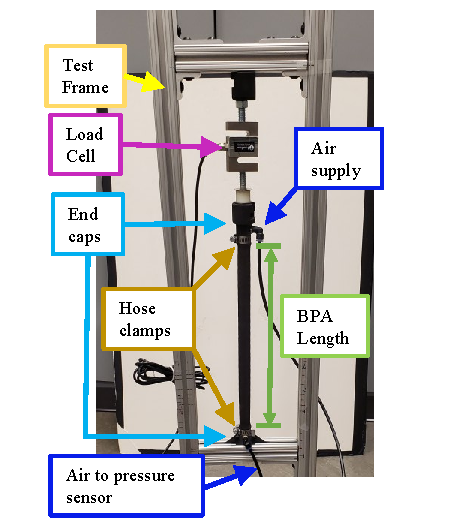
\includegraphics[width=0.75\textwidth]{01_testJigs1.pdf}
   \end{center}
    \caption{A picture of a BPA in the isometric force test stand with components labeled.}\label{fig:testJig}
\end{figure}

%%%%%%%%%%%%%%%%%%%%%%%%%%%%%%%%%%%%%%%%%%

\section{Robot Leg Model and Knee Test Stands}\label{sec:robot_model}


The primary components of the robot leg are the knee joint, femur, tibia, BPA assemblies, and artificial tendons (Fig. \ref{fig:testJigs}\textbf{A--C}). The artificial bone components are 3D printed using a combination of Onyx, carbon fiber, and high-strength high-temperature fiberglass on Markforged Onyx One and Mark Two printers. Onyx is a proprietary Markforged material that consists of chopped carbon fiber in nylon. Artificial tendons are made with Shimano bicycle brake cable. 
%3/16 inch braided steel wire rope for the $\phi$\qty{40}{\mm} BPAs. 

\begin{figure}[htbp]
    \begin{center}
    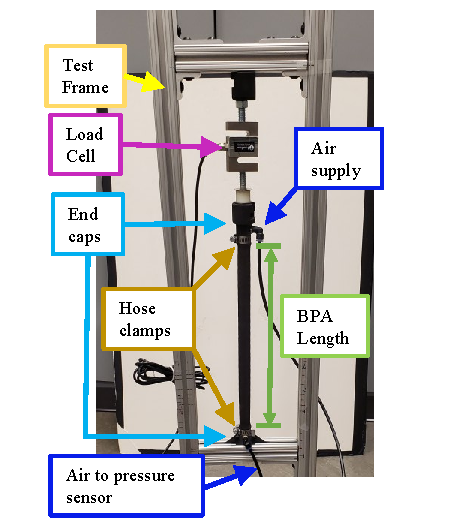
\includegraphics[width=0.9\textwidth]{testJigs.pdf}
    \end{center}
    \caption{\textbf{(A)} CAD solid model assembly of the revolute joint knee in the test stand. \textbf{(B)} 1-DoF pinned-joint robot knee in the test apparatus with important components labeled. Leg is shown with 30 degrees flexion, i.e. $\theta_\text{k} = \ang{-30}$. \textbf{(C)} Picture from isometric torque testing. Setup shows the revolute knee configured for a test of the extensor BPA. The knee is flexed with $\theta_\text{k} = \ang{-120}$. Also note the compressed shape of the inflated BPA on the knee during this high degree of flexion. }\label{fig:testJigs}
\end{figure}

The leg assembly geometry and dimensions are based on bones scans of a $6 \, \text{ft}$  (\qty{1.83}{\metre}) tall person \citep{bolen_determination_2019,seth_opensim_2018,delp_interactive_1990,delp_opensim_2007}. Two knee joints were tested, one pure rotational joint, and one biomimetic joint with rotation and translation. Each joint is driven by two antagonistic Festo actuators. Both robot joints have the same center of rotation in the femur frame at $\theta_\text{k}=0 \deg$.

Details on the biomimetic robot knee used in this study can be found in \cite{steele_biomimetic_2018,steele_development_2017,steele_biomimetic_2018-1}. In brief, this 1-DoF joint (Fig. \ref{fig:ICR}) uses a four-bar linkage to change the effective moment arm during rotation. The intersection point of the internal crossed links define the instantaneous center of rotation (ICR). This causes the joint ICR location in the femur frame to translate backwards in the $X$ and $Y$ directions \citep{wu_for_1995,wu_isb_2002} during knee rotation, similar to how the human knee behaves \citep{bolen_determination_2019,morrow_optimization_2020,seth_opensim_2018,delp_opensim_2007,delp_interactive_1990}. Correct location of the ICR is important for both theoretical and experimental torque calculations.

\begin{figure}[htbp]
    \begin{center}
    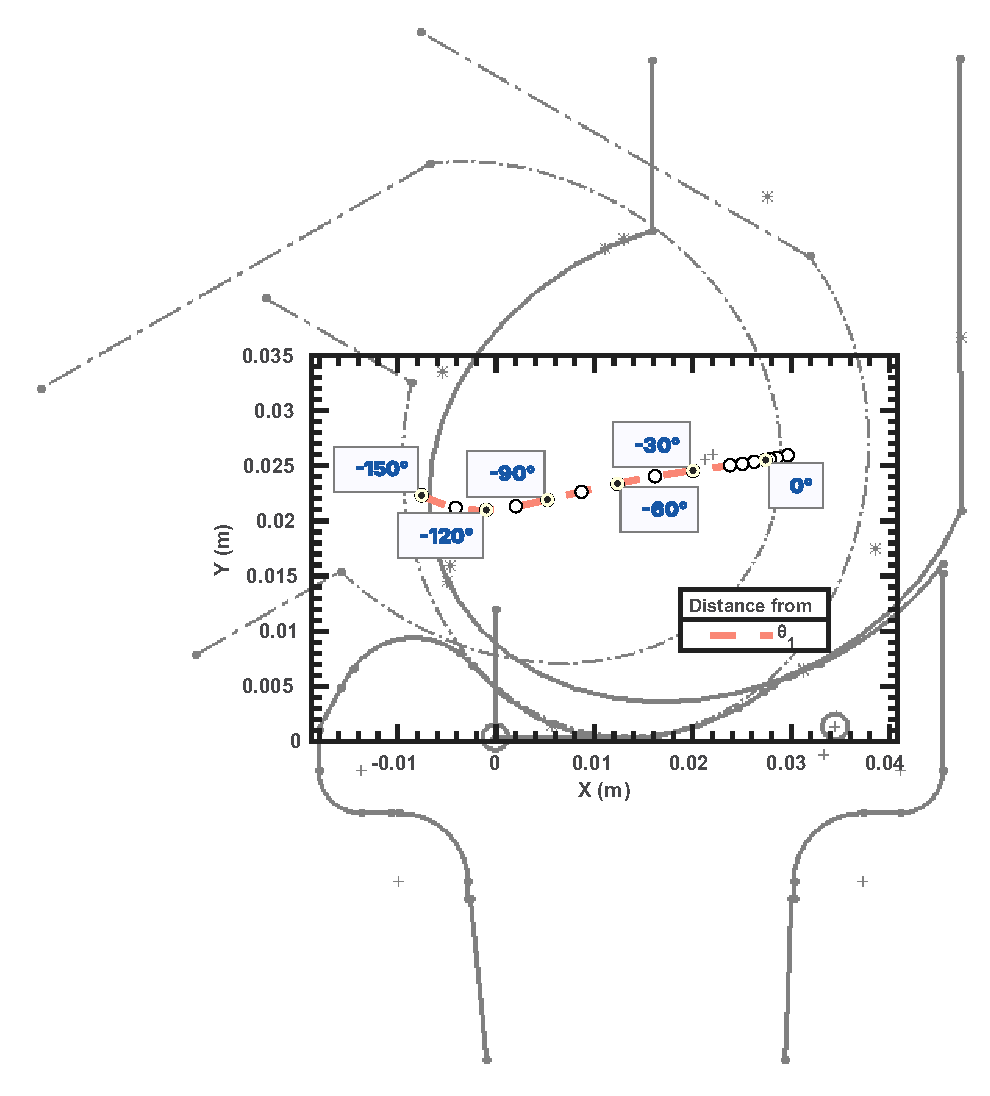
\includegraphics[width=0.8\textwidth]{KneeICR.eps}
    \end{center}
    \caption{ICR for biomimetic robot knee as a function of knee angle. Measured from $\theta_{1}$ on the tibia. Plot is overlayed on model of the knee at $\theta_\text{k}=0^\circ$ (solid line), and $-60^\circ$ and $-120^\circ$ (dotted dash lines). White circles represent measured points in $-15^\circ$ increments from $-150^\circ$ to $-15^\circ$, $-5^\circ$ increments from $-15^\circ$ to $0^\circ$, and then at $2^\circ$, $5^\circ$, and $10^\circ$.}\label{fig:ICR}
\end{figure}

One uniarticular knee extensor and one uniarticular knee flexor are used to actuate the joint. Each knee joint type was tested using $\phi$\qty{10}{\mm} Festo BPAs. Additionally, the biomimetic knee joint was tested using a $\phi$\qty{20}{\mm} Festo BPA. Each artificial muscle was pinned at the muscle origin location on the femur while the other end was either pinned or attached to the muscle insertion location on the tibia via an artificial tendon.

Moment arms are calculated using vector components between muscle locations and the joint center of rotation. Given a vector $\Vec{d}$ from a joint to the line of action of the force vector $\Vec{F}$, the moment arm $\Vec{r}$ is the shortest distance to this line of action. In this study, it is calculated using the method specified by Young and colleagues \citep{young_analyzing_2019}. The scalar moment arm, $r_{k}$, about the $z_{k}$ axis (i.e. the $Z$ axis in the knee frame) is calculated as 

\begin{equation}
    r_{k} = \Vec{p_{proj,xy}} \cdot \frac{\Vec{p_f} \times \hat{z_{k}}} { \norm{\Vec{p_f} \times \hat{z_{k}} }} \label{eq:project_ma}
\end{equation}

where $\Vec{p_{proj,xy}}$ is the free muscle segment projected onto the $XY$--plane, which is normal to the joint axis. $\Vec{p_f}$ is the projected muscle segment vector. Moment arm is calculated in the tibial body frame.

Full details of the existing model and the method to calculate torque in the modeled robot are given din \citep{bolen_determination_2019, morrow_optimization_2020}.


\section{Knee Torque Data Collection and Equipment}\label{sec:torque_equipment}


A test jig was built to collect knee torque measurements at different knee angles over its range of motion. The test stand frame is made predominantly out of 80/20\textsuperscript{\texttrademark} 1515 series extruded aluminum components. The knee joint is free to rotate the tibia while the femur is fixed to the frame. A force sensor has one end connected to the tibia and the other is connected to a swing arm. The swing arm is tied to a winch with $3/16\; \text{inch}$ Kevlar rope from Quality\texttrademark \: Nylon Rope routed over intermediate idler pulleys (see Fig. \ref{fig:testJigs}\textbf{B} and \ref{fig:testJigs}\textbf{C}). At each measured position of $\theta_{k}$ the winch would be locked and the BPA would be inflated and then deflated. This test procedure kept the measured results as isometric as possible.  The knee joint is co-axial with gravity to eliminate gravitational torque (see Fig. \ref{fig:testJigs}\textbf{A} and Fig. \ref{fig:testJigs}\textbf{C}).

Force data was collected using one of two different sensors. The first is a MODERN STEP $\qty{300}{\kilo\gram}$ digital crane scale. The second force sensor is a CALT DYLY-103 $\qty{100}{\kilo\gram}$ S shaped load cell. The load cell is used in conjunction with a HX711 Load Cell Amplifier. Pressure is measured with a Freescale MPX5700 GP $\qty{5}{\volt}$ pressure sensor. Building air supply pressure is controlled with two pressure regulators in series. The first is a Parker model 20R113GC $0-120\; \text{psi}$ pressure regulator. The second is a Husky $3/8 \; \text{inch}$ High Performance Air Regulator HDA72200. A Festo VTUG-10-MRCR-S1T-26V20-T516LA-UL-T532S-8K valve manifold was used to supply air to the actuator. Pressure and load cell amplifier data are sent to Matlab via an Arduino Uno style Sparkfun BlackBoard C microcontroller. 

%The computers that used Matlab were running either Windows 10 and Windows 11.During phases when the Arduino was collecting $F$ and $P$ data to send to Matlab, the Arduino would also trigger (via Matlab) an Onsemi 2N4401 NPN transistor to make valve manifold open or close the valve. For other data collection the valve was manually opened and closed.

The length measurements were made using a tape measure. When there was sufficient curvature in the BPA during knee extensor torque tests, a flexible piece of string was used to mark the axial length and then transferred to the tape measure. Angle measurements were taken with a Medigauge digital electronic goniometer or with MALENOO analog goniometers of 6, 8, or 12 inch lengths.  


\section{Hybrid Torque Calculation Method}\label{sec:hybrid_method}


A Hybrid Torque calculation method was developed to help uncover inconsistencies between the model and recorded torque values. This method measures the actual muscle length and angles of the robot to calculate force and joint torque. With this method, it is easier to determine which parts of the torque equation did not achieve their predicted value and provide a correction to that part of the equation. The classical mechanics way to calculate the torque $\Vec{M}$, about a joint is to take the cross product of distance, $\Vec{d}$, and force, $\Vec{F}$

\begin{equation}
    \Vec{M} = \Vec{d} \times \Vec{F} \label{eq:M_vec}
\end{equation}

where distance $\Vec{d}$ and force $\Vec{F}$ are described in the previous section. Knee torque is the scalar torque $M$ about the $Z$ axis, which can simplify Eq. \ref{eq:M_vec} to

\begin{equation}
    M = r \times F \label{eq:M_scalar}
\end{equation}

where $r$ is the moment arm measured by a tape measure, and $F$ is the scalar force, calculated by measuring the BPA's $P$, $l_{0}$, $l_{620}$ and $l_\text{m}$ values and using the model fit equations determined in the following section.



\section{Improved Torque Model}\label{sec:improved_model}

The classical kinematic torque model assumed rigid links and inextensible muscle paths. Data collected during the first flexor experiments (Chapter~\ref{ch:results}) showed that this assumption does not hold for a pneumatic system: measured muscle lengths were consistently shorter than predicted, and measured torque deviated from prediction in a load-dependent manner. This section describes the corrections that were developed to account for a constant length offset, series compliance in the attachment hardware and artificial tendons, and the loss of usable muscle length when a BPA wraps around the joint.

Analysis of measured muscle length data shows that it was consistently shorter than the predicted muscle length at all joint angles. This shorter length results in less muscle force, a shifted RoM, and less torque in the experimental setup. That this shorter length occurs when $\varepsilon=1$ and $F=0$ indicates that a constant length offset should be used. Therefore, to produce an improved torque prediction model, $l_\text{m}$ was recalculated as

\begin{equation}
    l_\text{m} = l_{LMT} - 2\;l_{fitting} - \chi_{0} 
    \label{eq:Lm}
\end{equation}

where $l_{LMT}$ is the path length of the musculotendon from origin to insertion point, $l_{fitting}$ is the length of the end caps, and $\chi_{0}$ is a constant length offset. 

Additionally, as the muscles produce more force, compliant components in the limb segments and attachment hardware deform. This deformation changes the effective braided pneumatic actuator (BPA) length, which alters contraction and therefore changes the force predicted by the BPA model. This effect is most apparent at high forces and low contractions. To correct this error, we approximated the combined hardware compliance using Hooke's law in the bracket's principal directions.

A local bracket frame was established at the attachment bracket. The $\hat{x}_{br}$ direction was aligned with the vector from the bracket reference point to the BPA attachment point and represents the stiffest direction of the bracket. The $\hat{y}_{br}$ direction was chosen to point in the posterior direction with respect to the tibia frame, corresponding to the primary cantilever bending direction (see Fig.~\ref{fig:bktFrame}), while the $\hat{z}_{br}$ direction completes the right-handed frame. The bracket stiffness matrix is modeled as a diagonal matrix to reflect independent stiffness components along its principal axes:

\begin{equation}
\mathbf{K}_{br} = 
\begin{bmatrix}
\chi_{1} & 0   & 0 \\
0   & \chi_{2} & 0 \\
0   & 0   & \chi_{1} \\
\end{bmatrix}
\label{eq:bktstiffness}
\end{equation}

The corresponding local compliance matrix is 

\begin{equation}
\mathbf{C}_{br} = \mathbf{K}_{br}^{-1}
\label{eq:bktcompliance}
\end{equation}

Force that doesn't account for deformation is $\mathbf{F}$. The force applied to the bracket was expressed in the bracket frame as $\mathbf{F}'$. This force vector can be written in terms of its magnitude and unit direction as

\begin{equation}
\mathbf{F}' = \left\| \mathbf{F}' \right\| \hat{\mathbf{u}}
\label{eq:bktforcevector}
\end{equation}

where $\hat{\mathbf{u}} = [u_{x}, u_{y}, u_{z}]^{T}$ is the BPA force direction expressed in the bracket frame. The bracket deflection vector, $\boldsymbol{\epsilon}_{br}$, was calculated from Hooke's law as 

\begin{equation} \mathbf{F}' = \mathbf{K}_{br} \: \boldsymbol{\epsilon}_{br}
\label{eq:bktvectorhooke}
\end{equation}

Solving Eq. \ref{eq:bktvectorhooke} for the bracket deflection gives

\begin{equation}
\boldsymbol{\epsilon}_{br} = \mathbf{K}_{br}^{-1} \: \mathbf{F}' = \mathbf{C}_{br} \: \mathbf{F}'
\label{eq:bktdeflection}
\end{equation}

Substituting Eq. \ref{eq:bktforcevector} into Eq. \ref{eq:bktdeflection} gives

\begin{equation}
\boldsymbol{\epsilon}_{br} = \left\| \mathbf{F}' \right\| \mathbf{K}_{br}^{-1} \,\hat{\mathbf{u}}
\label{eq:bktdeflectionforceunit}
\end{equation}

For the diagonal stiffness matrix in Eq. \ref{eq:bktstiffness}, Eq. \ref{eq:bktdeflection} is equivalent to the component-wise expression

\begin{equation}
\boldsymbol{\epsilon}_{br} = \begin{bmatrix} F'_{x,br}/\chi_{1} \\ F'_{y,br}/\chi_{2} \\ F'_{z,br}/\chi_{1} \end{bmatrix}
\label{eq:bktcomponentdeflection}
\end{equation}

Although $\boldsymbol{\epsilon}_{br}$ is a three-dimensional deflection vector, the BPA force model depends on the scalar change in effective BPA length ($\delta$). Therefore, only the component of $\boldsymbol{\epsilon}_{br}$ along the BPA line of action directly changes the effective BPA length. This scalar bracket deflection is the projection of $\boldsymbol{\epsilon}_{br}$ onto $\hat{\mathbf{u}}$:

\begin{equation}
{\delta}_{br} = \hat{\mathbf{u}}^{T} \boldsymbol{\epsilon}_{br}
\label{eq:bktprojecteddeflection}
\end{equation}

Substituting Eq. \ref{eq:bktdeflection} into Eq. \ref{eq:bktprojecteddeflection} gives

\begin{equation}
{\delta}_{br} = \hat{\mathbf{u}}^{T} \, \mathbf{K}_{br}^{-1} \, \mathbf{F}'
\label{eq:bktprojecteddeflection2}
\end{equation}

Using Eq. \ref{eq:bktforcevector}, Eq. \ref{eq:bktprojecteddeflection2} becomes

\begin{equation}
\delta_{br} = \left\| \mathbf{F}' \right\| \hat{\mathbf{u}}^{T} \, \mathbf{K}_{br}^{-1} \, \hat{\mathbf{u}}
\label{eq:bktprojectedcompliance}
\end{equation}

The scalar stiffness along the BPA line of action due to the bracket compliance is therefore

\begin{equation}
k_{\hat{u},br} = \frac{\left\| \mathbf{F}' \right\|}{\delta_{br}} = \left( \hat{\mathbf{u}}^{T} \mathbf{K}_{br}^{-1} \hat{\mathbf{u}} \right)^{-1}
\label{eq:keff}
\end{equation}

This projected-compliance form is used because the force is applied along $\hat{\mathbf{u}}$, while the bracket is allowed to deflect independently along its local $\hat{x}$, $\hat{y}$, and $\hat{z}$ directions. The reduced-order Hooke's law expression for the bracket deflection along the BPA line of action is therefore

\begin{equation} \left\| \mathbf{F}' \right\| = k_{eq} \: \delta
\label{eq:hookereduced}
\end{equation}

where $k_{eq}$ is calculated with \eqref{eq:keff} when there is no artificial tendon. When an artificial tendon was used, it was modeled as an axial spring with stiffness $k_{ten}$. Since both bracket deflection and tendon stretch reduce the effective BPA length along the actuator line of action, their scalar compliances were added in series:

\begin{equation} k_{eq} = \left( \frac{1}{k_{br}} + \frac{1}{k_{ten}} \right)^{-1}
\label{eq:equivalentstiffness}
\end{equation}

Since $\delta$ is the scalar compliance displacement along the BPA line of action, then the compliance-corrected active BPA length used in the force balance is

\begin{equation} l_m(\delta) = l_m^{(0)} - \delta
\label{eq:activelengthcorrected}
\end{equation}

where $l_m^{(0)}$ is calculated from \eqref{eq:Lm}.

The corresponding relative contraction is $\varepsilon^*(\delta)$. Since the BPA force depends on contraction, and contraction depends on the compliance displacement, $\delta$ was found using the Newton-Raphson method to solve the nonlinear force-balance equation

\begin{equation} F_{\mathrm{max}} \cdot F_{\mathrm{BPA}}\!\left(\varepsilon^*(\delta),P^*\right) - k_{eq}\,\delta = 0
\label{eq:complianceforcebalance}
\end{equation}

After solving Eq. \ref{eq:complianceforcebalance}, the corresponding force magnitude was used in Eq. \ref{eq:bktdeflection} to compute the vector bracket deflection. This deflection was transformed back into the limb reference frame and used to update the BPA attachment location. The routed BPA length, force direction, moment arm, and torque were then recalculated using the updated attachment location. In the present implementation, the optimized stiffness terms $\chi_{1}$ and $\chi_{2}$ were treated as effective compliance parameters for the attachment system rather than direct measurements of an isolated bracket. This allowed unmodeled compliance in the surrounding hardware to be represented by the reduced-order stiffness model.



\begin{figure}[htbp]
\begin{center}
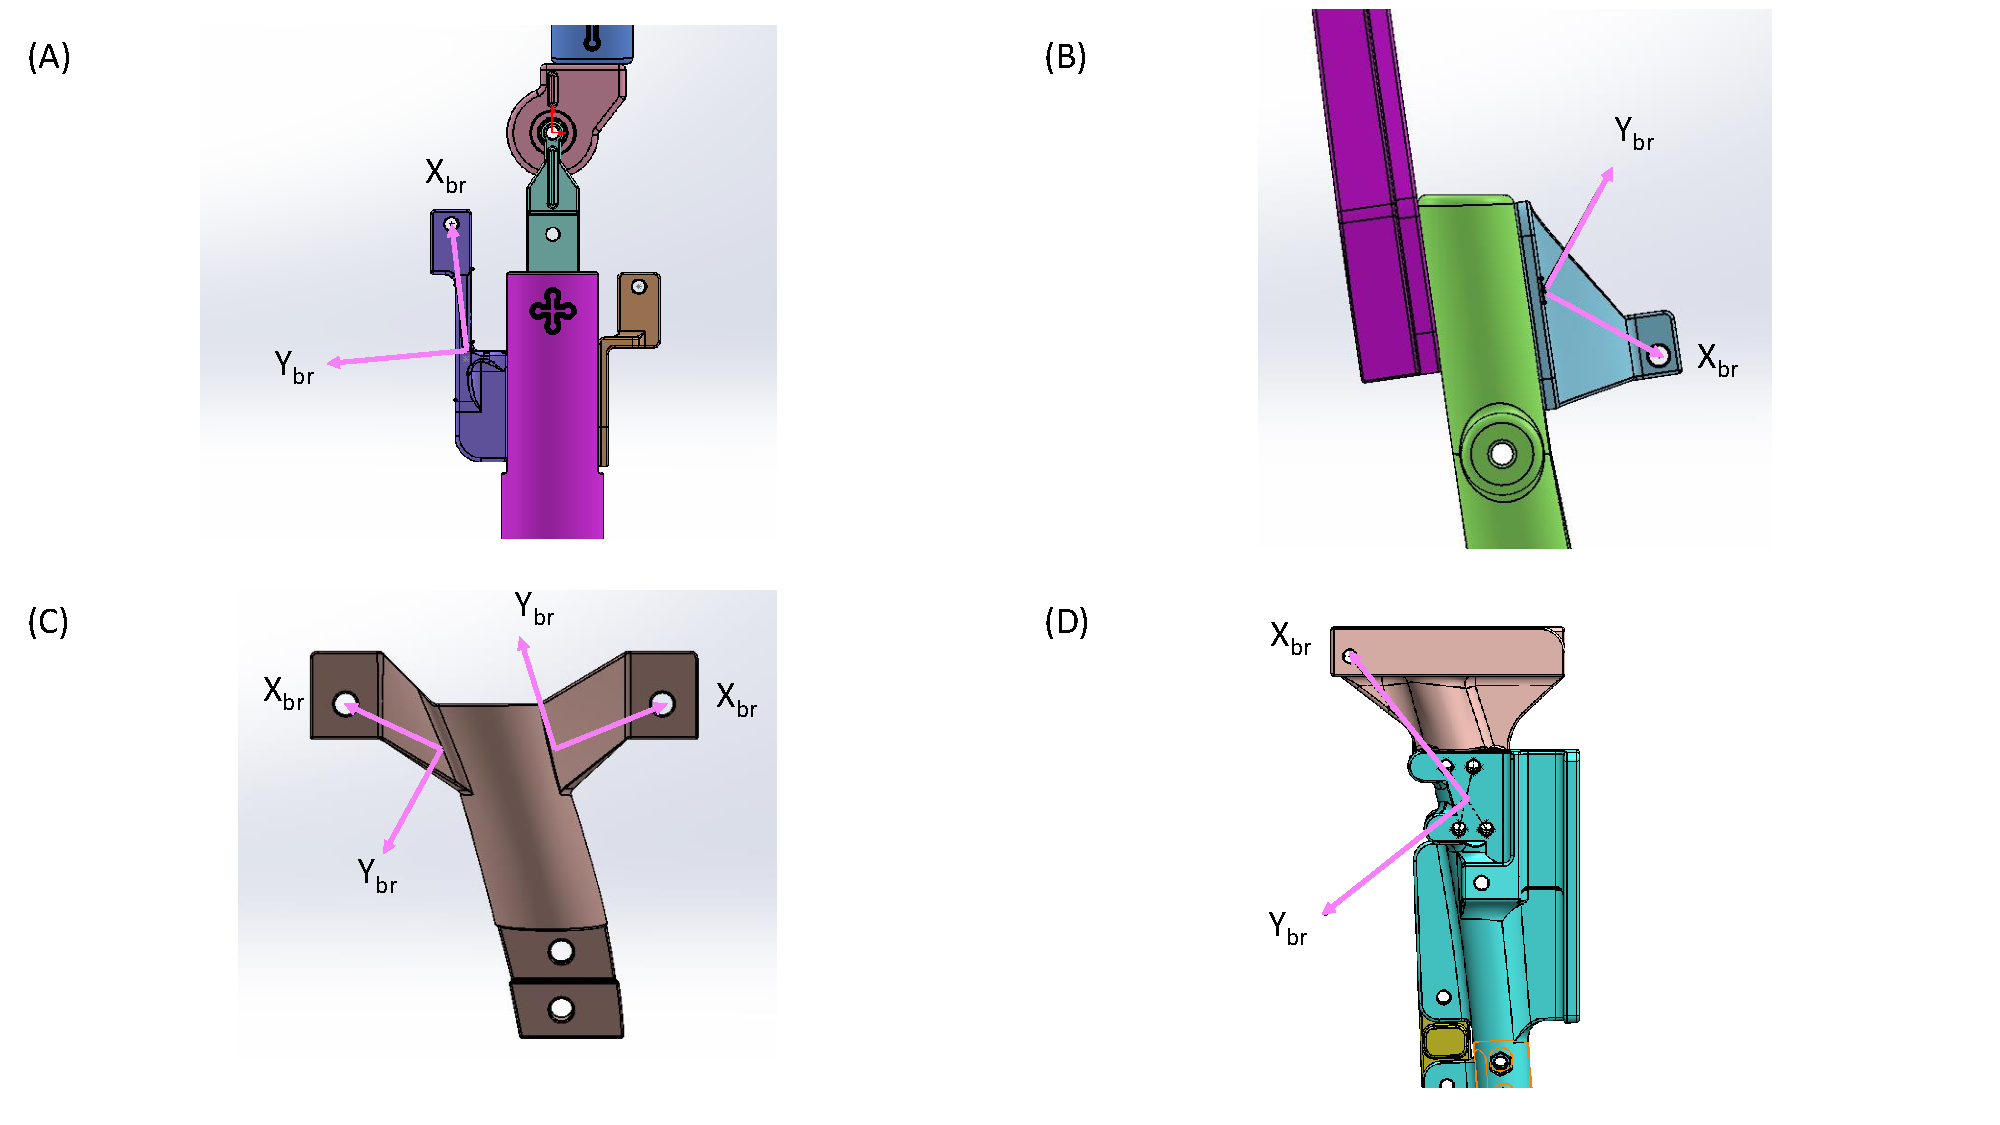
\includegraphics[width=1\textwidth]{bktFrame.pdf}
\end{center}
\caption{Bracket frame orientations for: \textbf{(A)} Flexor configuration on the pinned knee, \textbf{(B)} extensor configuration on the pinned knee, \textbf{(C)} flexor and extensor configurations on the biomimetic knee with $\phi$\qty{10}{\mm} BPAs, and \textbf{(D)} flexor configuration on the biomimetic knee with the $\phi$\qty{20}{\mm} BPA.}
\label{fig:bktFrame}
\end{figure}

Multiobjective optimization using \texttt{gamultiobj} in Matlab was used to determine the length offset ($\chi_{0}$) and the stiffness terms ($\chi_{1}$ and $\chi_{2}$) until the error between the model and the experimental data was minimized for the $l_{0}=\qty{48.5}{\cm}$ flexor BPA (Fig.~\ref{fig:FlxPin_group}\textbf{C}). Because the bracket forms an arch shape and extends for \qty{75}{\mm} in the $Z$ direction, the extensor configuration required an additional correction. The inner side of a BPA that bends over the joint experiences less tensile stress than the outer side, creating a force imbalance and a loss of part of the arc length of the BPA as usable length. An additional optimization term $\chi_{3}$ was introduced to capture this wrapping loss, such that
\begin{equation}
    \Delta l = \begin{cases}
     \chi_{3}\;R\;\abs{ \theta_\text{wrap}-\theta_\text{k}}\;\zeta^2 & \theta_\text{k} \leq      \theta_\text{wrap} \\
      0 & \theta_\text{k} \geq \theta_\text{wrap}
     \end{cases}\label{eq:deltaL}
\end{equation}

where $\Delta l$ is the change in usable length of the BPA, $R$ is the wrapping radius. $\theta_\text{wrap}$ is the knee flexion angle when the BPA starts to bend over the knee joint, determined from solid modeling. $\zeta$ is the additive complement to relative strain, such that

\begin{equation}
    \zeta = 1-\varepsilon^*  \\
\label{eq:comp}
\end{equation}

Combining \eqref{eq:comp} into \eqref{eq:deltaL}, and subtracting $\Delta l$ from  \eqref{eq:Lm} yields

\begin{equation}
    l_\text{m} = l_{LMT} - 2\;l_{fitting}  - \chi_{0} - \Delta l\label{eq:x3}
\end{equation}

The optimization algorithm was again gamultobj in Matlab. This time, the muscle origins bracket was chosen. The bracket frame is shown in Fig. \ref{fig:bktFrame}\textbf{B}. Since the bracket forms an arch shape and extends for \qty{75}{\mm} in the $Z$ direction, for this configuration only we set $K_{2}$ in the $X_{br}$ direction, and $K_{1}$ in the $Y_{br}$ and $Z_{br}$ directions. The optimization algorithm for this set solves for the best average goodness-of-fit (GoF) measures RMSE, FVU, and maximum absolute residual for two BPAs, while the third one was held out. Three independent rounds of optimization were performed, so that one of each of the BPAs could be held out as validation. Then we picked the solution with the shortest distance between the average normalized GoF and the validation data, while also requiring improved GoF values for all the individual BPAs, with the exception of maximum absolute residual on the $l_{0}=\qty{48.0}{\cm}$ BPA.

The goodness-of-fit metrics used to judge the optimization results are the root mean square error (RMSE), the fraction of variance unexplained (FVU), and the maximum absolute residual, each computed between the measured and predicted isometric torque over the tested range of motion.

\chapter{Results}\label{ch:results}

{\doublespacing\normalsize\upshape
\noindent Publication note: Section~\ref{sec:results_force} and the associated figures and tables appeared in \citet{bolen_2026} (Bolen, Elzein, Pang, and Hunt, \emph{Actuators}, 2026). Section~\ref{sec:results_torque} and the associated figures and tables are also the subject of an unpublished manuscript in preparation by Bolen, Burgess, Morrow, Elzein, Pang, Scharzenberger, and Hunt \citep{bolen_isometric_2025}. This manuscript has not been submitted for publication. Author contributions for both works are stated in Chapter~\ref{ch:methods}.\par}

\section{BPA Force Characterization}\label{sec:results_force}

This section reports the results of the isometric force characterization experiments described in Section~\ref{sec:force_experiment}. First, maximum isometric force at \qty{620}{\kPa} is modeled as a function of resting length. The remaining data are then normalized to build a predictive force surface, and the resulting model is compared with the manufacturer's tool and with other published BPA models.


\subsection{Maximum Force at 620 kPa}

Data of the maximum force from BPA characterization tests of the \qty{10}{\mm} and \qty{20}{\mm} diameters at \qty{620}{\kPa} show a dependency on resting length (Figure~\ref{fig:Fmax_fit}). This is a previously unreported characteristic of these artificial muscles. Detailed analysis of the Festo \mbox{tool \citep{festo_2026}} does in fact predict a change in maximum force with the resting length; however, the Festo tool predicts increased force with shorter lengths, while our collected data indicate decreasing force with shorter lengths. The data show a force response resembling an $\arctan$ curve along the $l_0$ dimension. Using the Nonlinear Least Squares method and a Least Absolute Residual robustness, we fit an arctan curve to the data to get the maximum force at \qty{620}{\kPa} given a resting length as:
\begin{align}
    F_{620_{10}} &= \qty{303.5}{\N}\cdot \arctan{( \qty{19.03}{\per\metre} \cdot (l_0-0.0075))}  \label{eq:Fmax10} \\[10pt]
    F_{620_{20}} &= \qty{922.4}{\N} \cdot \arctan{(\qty{15.37}{\per\m} \cdot (l_0-0.013))} \label{eq:Fmax20}
\end{align}

\noindent
The length is offset by \qty{0.0075}{\m} and \qty{0.013}{\m} because solid modeling showed that the end caps contact each other at these lengths. At these lengths, the actuator would not be able to contract to produce force.


\begin{figure}[H]%[tbp]
%\begin{adjustwidth}{-\extralength}{0cm}
%\centering
\subfloat[\centering]{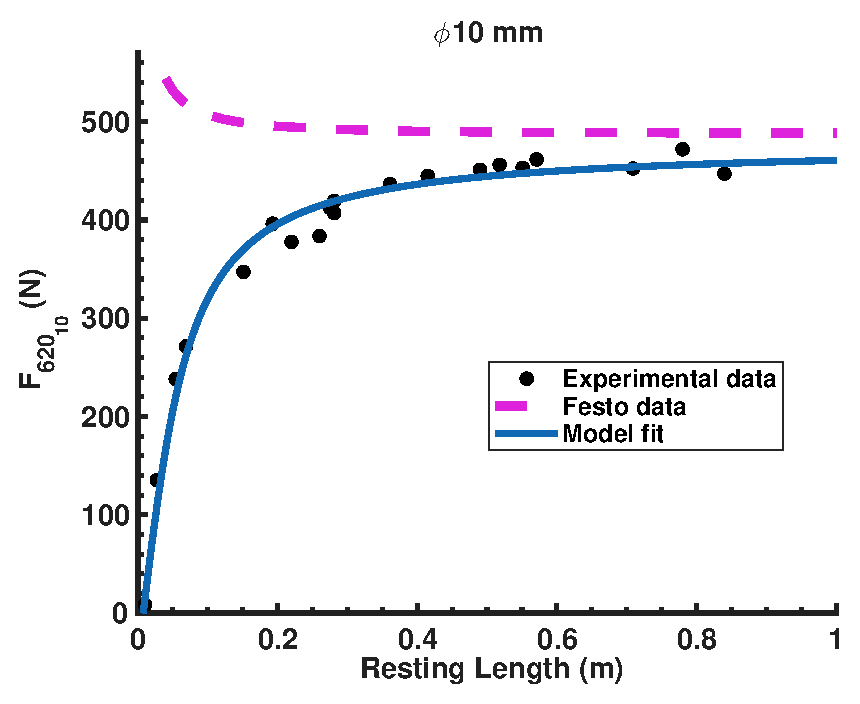
\includegraphics[width=13.8cm]{02a_MaxForce10.eps}}\\
\subfloat[\centering]{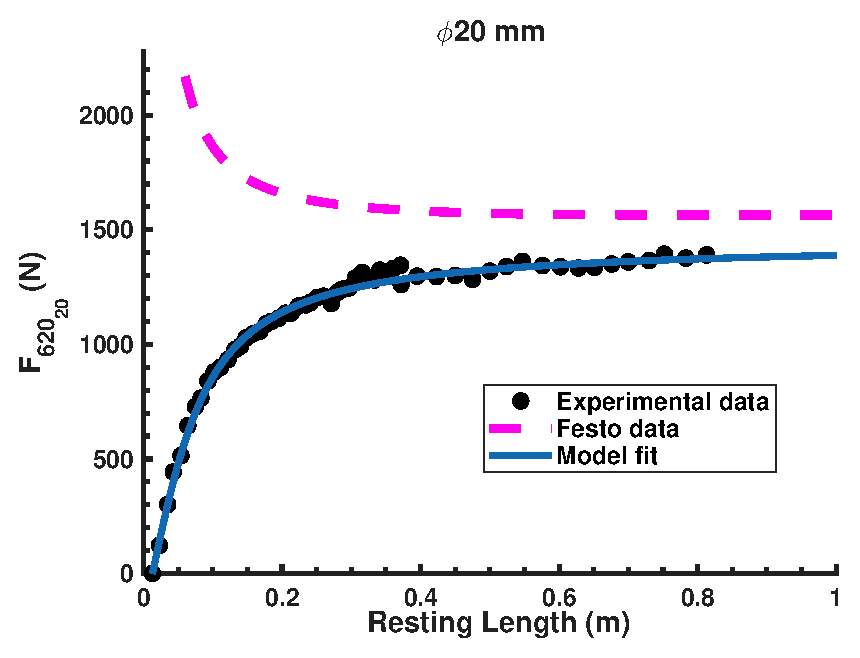
\includegraphics[width=13.8cm]{02b_MaxForce20.eps}}
%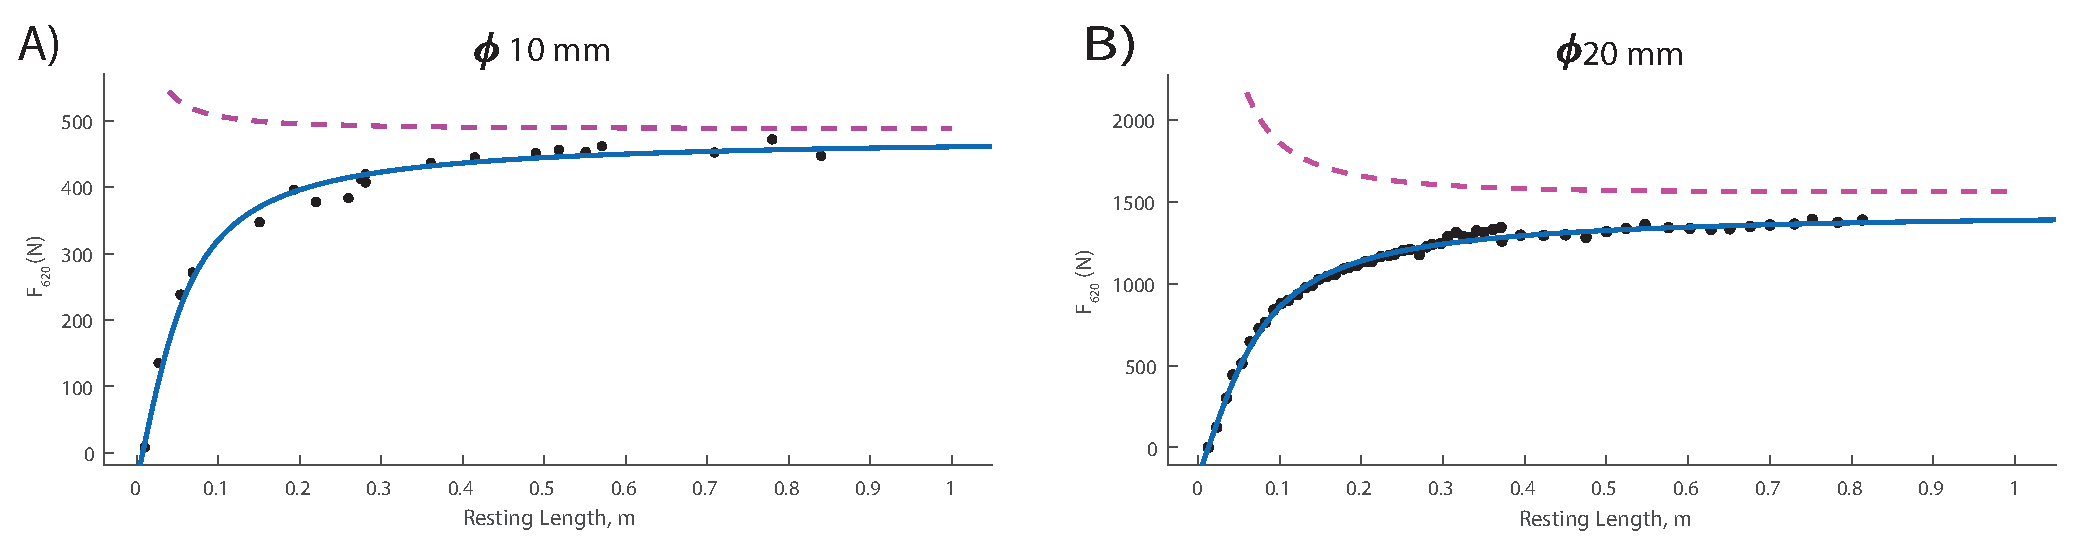
\includegraphics[width=1\textwidth]{02_Fmax_fit.eps}
%\end{adjustwidth}
\caption{Results for finding the relationship between $F_{620}$ and $l_0$. (\textbf{a}) $F_{620_{10}}$ as a function of $l_0$, at $P_{620}$. Dashed line is the $F_{620_{10}}$ data from Festo. Solid line is the fit from Equation (\ref{eq:Fmax10}). (\textbf{b}) $F_{620_{20}}$ as a function of $l_0$ at $P_{620}$. Dashed line is $F_{620_{20}}$ data from Festo. Solid line is the fit from Equation (\ref{eq:Fmax20}).}\label{fig:Fmax_fit}
\end{figure}


%Data from BPA characterization tests of the \qty{10}{\mm} muscles resulted in force-pressure pairings for different muscle resting lengths ($l_0$) Figure~\ref{fig:Fmax_fit}\textbf{A}. Analysis of the data showed that the maximum isometric force ($F_{max}$) produced by the actuator at its resting length is a function of resting length $l_0$ (Figure~\ref{fig:Fmax_fit}B), a previously unreported characteristic of these artificial muscles. The data show a force response resembling an $\arctan$ curve along the $l_0$ dimension and with a more linear response with changes in pressure. Using the Nonlinear Least Squares method and a Least Absolute Residual robustness, we fit an arctan curve to the data at to get the maximum force given a resting length and pressure as:

\subsection{Force as a Function of Pressure and Resting Length}

Data from BPA characterization tests of the \qty{10}{\mm} muscles resulted in force--pressure pairings for different muscle resting lengths ($l_0$) (Figure~\ref{fig:F-P_contraction}a). Similar to the maximum force data, these data show a force response resembling an $\arctan$ curve along the $l_0$ dimension  with a more linear response to changes in pressure. Using the Nonlinear Least Squares method and a Least Absolute Residual robustness, we fit an arctan curve to the data to get the maximum force given a resting length and pressure as described by the model form given in Section~\ref{sec:force_model}:
where $a_1 = \qty{0.4895}{\N\per\kPa}$  and $a_2=\qty{0.03068}{\per\kPa\per\m}$ for the \qty{10}{\mm} actuator, and \mbox{$a_1 = \qty{1.49}{\N\per\kPa}$,} $a_2=\qty{0.0248}{\per\kPa\per\m}$ for the \qty{20}{\mm} actuator. Goodness-of-fit measures are given in Table~\ref{tab:Fmax}. 



\begin{table}[H]
\caption{Maximum force equation coefficient values with confidence intervals (CI) and goodness-of-fit measures. Equation~(\ref{eq:Fmax_3D}) is compared to data taken at \qty{620}{\kPa} . Equations~(\ref{eq:Fmax10}) and (\ref{eq:Fmax20}) are compared against maximum force from using the Festo tool. It was not necessary to fit an adjusted $\text{R}^2$ in \mbox{these cases.}} 
\label{tab:Fmax}
\tiny
\begin{adjustwidth}{0cm}{0cm}
%\centering %% If there is a figure in wide page, please release command \centering
\begin{tabularx}{\textwidth}{cllllrclr}
\toprule
\multirow{2}{*}{\textbf{Equation}} &
  \multirow{2.1}{*}{\textbf{Coefficient}} &
  \multirow{2.2}{*}{\textbf{CI (95\%)}} &
  \multicolumn{3}{c}{\textbf{Our Model}} &
  \multicolumn{3}{c}{\textbf{Festo Tool}} \\  
 &
   &
   &
  \multicolumn{1}{l}{\textbf{Adj. $\text{R}^2$}} &
  \multicolumn{1}{l}{\textbf{RMSE}} &
  \textbf{Max. Error} &
  \multicolumn{1}{l}{\textbf{Adj. $\text{R}^2$}} &
  \multicolumn{1}{l}{\textbf{RMSE}} &
  \textbf{Max. Error} \\ \midrule 
\multirow{2}{*}{\eqref{eq:Fmax_3D}} &
  $a_1 =   \qty{0.4895}{\N\per\kPa}$ &
  (0.4822, 0.4968) &
  \multicolumn{1}{l}{\multirow{2}{*}{0.9945}} &
  \multicolumn{1}{l}{\multirow{2}{*}{11.61 N}} &
  \multirow{2}{*}{55.3 N} &
  \multicolumn{1}{l}{\multirow{2}{*}{0.9854}} &
  \multicolumn{1}{l}{\multirow{2}{*}{14.7 N}} &
  \multirow{2}{*}{30.9 N} \\ 
 &
  $a_2 =   \qty{0.03068}{\per\kPa\per\m}$ &
  (0.0282, 0.03317) &
  \multicolumn{1}{l}{} &
  \multicolumn{1}{l}{} &
   &
  \multicolumn{1}{l}{} &
  \multicolumn{1}{l}{} &
   \\ \midrule
\multirow{2}{*}{\eqref{eq:Fmax10}} &
  $b_1   =\qty{303.5}{\N}$ &
  (300, 308) &
  \multicolumn{1}{l}{\multirow{2}{*}{0.9854}} &
  \multicolumn{1}{l}{\multirow{2}{*}{14.72 N}} &
  \multirow{2}{*}{30.9 N} &
  \multicolumn{1}{c}{\multirow{2}{*}{--}} &
  \multicolumn{1}{l}{\multirow{2}{*}{189.9 N}} &
  \multirow{2}{*}{375.6 N} \\ 
 &
  $b_2 =   \qty{19.03}{\per\m}$ &
  (17.48, 20.57) &
  \multicolumn{1}{l}{} &
  \multicolumn{1}{l}{} &
   &
  \multicolumn{1}{l}{} &
  \multicolumn{1}{l}{} &
   \\ \midrule
\multirow{2}{*}{\eqref{eq:Fmax20}} &
  $b_1 =   \qty{922.4}{\N}$ &
  (914.2, 930.7) &
  \multicolumn{1}{l}{\multirow{2}{*}{0.9945}} &
  \multicolumn{1}{l}{\multirow{2}{*}{23.83 N}} &
  \multirow{2}{*}{62.1 N} &
  \multicolumn{1}{c}{\multirow{2}{*}{--}} &
  \multicolumn{1}{l}{\multirow{2}{*}{668.4 N}} &
  \multirow{2}{*}{1590.1 N} \\ 
 &
  $b_2=\qty{15.37}{\per\m}$ &
  (14.75, 15.98) &
  \multicolumn{1}{l}{} &
  \multicolumn{1}{l}{} &
   &
  \multicolumn{1}{l}{} &
  \multicolumn{1}{l}{} &
   \\ \bottomrule
\end{tabularx}
\end{adjustwidth}
\end{table}



\subsection{Maximum Contraction at \qty{620}{\kPa}}

Figure~\ref{fig:F-P_contraction}(b) shows an attempt at a linear fit for maximum contraction at \qty{620}{\kPa} ($\epsilon_{620}$) as a function of resting length ($l_0)$. Error bars have been included to show the effect of $\pm$\qty{1}{\mm} accuracy with measurements of $l_0$ and $l_{620}$. There was a large amount of variance in the data, with the linear fit giving an adjusted $\text{R}^2=0.4124$ and an $\text{RMSE}=0.0083$. Since there is no direct, predicable relationship between maximum contraction and $l_0$, this value should be recorded in each muscle used on a robot to best predict the force it may produce at different pressures and contraction. 


\subsection{Force as a Function of Pressure and Contraction}

In addition to being a function of the pressure and resting length, the force produced by the actuator is also a function of the amount of actuator contraction, with less force being applied as the actuator contracts. 
To build this model, the collected data of force, pressure, and contraction are normalized by dividing by $F_{620}$, $P_{620}$, and $\epsilon_{620}$, respectively. This had the effect of compressing the data into a 3D surface ranging from 0 to 1 on all axes. Normalized data are compared with pressure isoclines of force predicted by the Festo tool divided by the maximum force equation described in the previous section in Figure~\ref{fig:GenForceFit}. With this comparison, it is clear that the Festo tool over-predicts the expected force, especially at lower pressures, contraction, and resting lengths.  






\begin{figure}[H]%[tbp]
%\begin{adjustwidth}{-\extralength}{0cm}
%\centering
\subfloat[\centering]{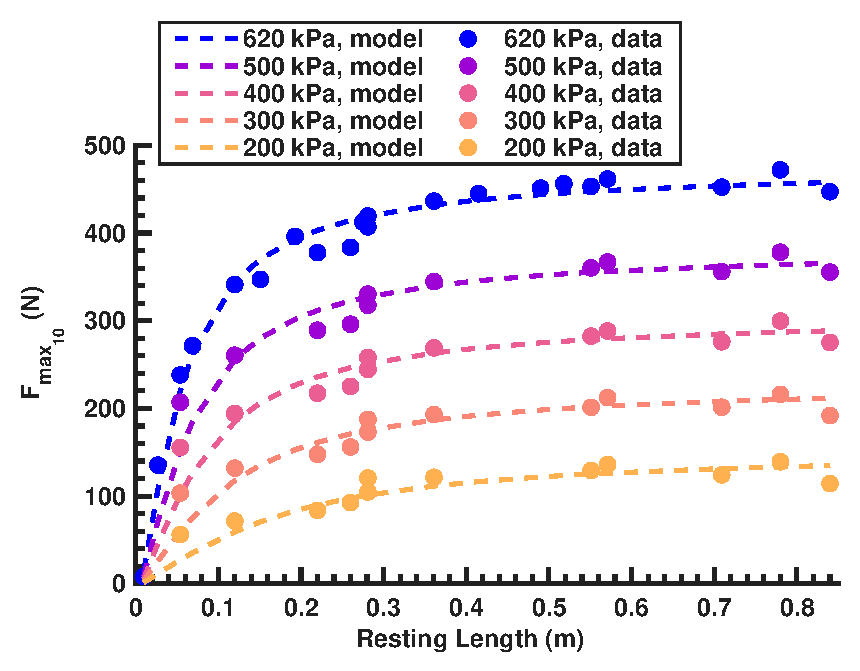
\includegraphics[width=13.3cm]{03a_MaxForce10_all.eps}}\\
\subfloat[\centering]{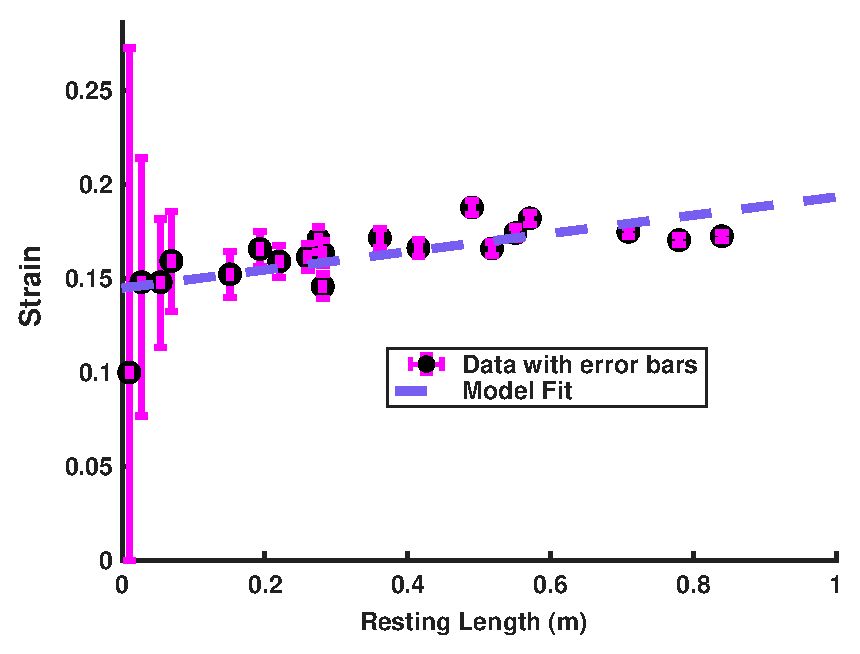
\includegraphics[width=13.8cm]{03b_kmax10.eps}}
%\end{adjustwidth}
\caption{Results for finding the relationship between $F_{620}$, $l_0$, $P_{620}$, and $\epsilon_{620_{10}}$. (\textbf{a}) Isoclines of the surface fit for $F_{620_{10}}(l_0,P_{620})$. (\textbf{b}) $\epsilon_{620_{10}}$ versus $l_0$ at $P_{620}$. Although there is a general trend of longer resting lengths producing more contraction, no conclusive relationship between $\epsilon_{620}$ and $l_0$ could be deduced from this experiment. The error bars show the effect of being $\pm$\qty{1}{\mm} in measuring $l_0$ and $l_{620}$.}\label{fig:F-P_contraction}
\end{figure}





\begin{figure}[H]%[tbp]
%\begin{adjustwidth}{-\extralength}{0cm}
%\centering
\subfloat[\centering]{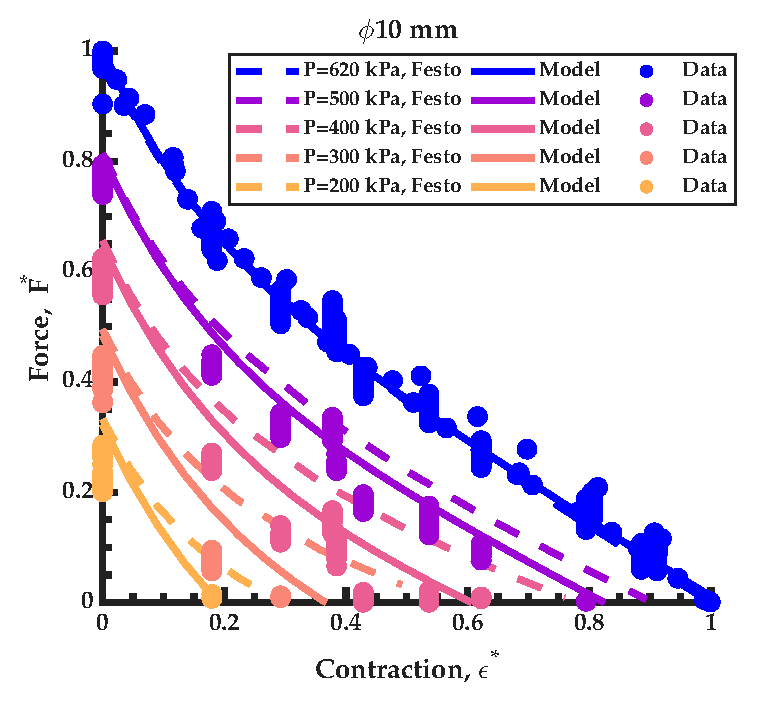
\includegraphics[width=10.88cm]{04a_FStar10.eps}}\\
\subfloat[\centering]{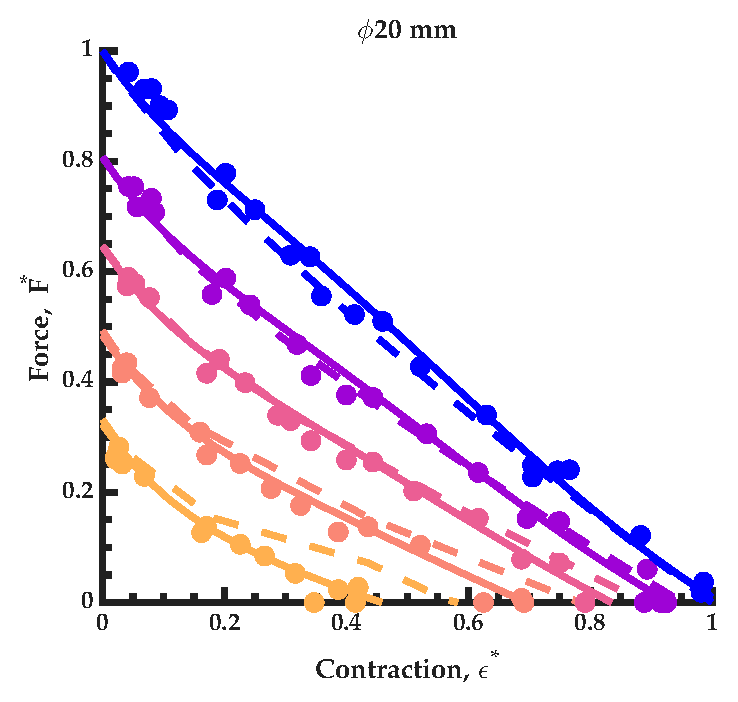
\includegraphics[width=10.88cm]{04b_FStar20.eps}}
%\end{adjustwidth}
\caption{Surface fit for $F^*(\epsilon^*,P^*)$. Solid lines are from our model. Dashed lines from Festo supplied data. In total, 537 data points were collected and used to fit the 3D surfaces (321 data points for $\phi$\qty{10}{\mm} BPAs and 216 data points for $\phi$\qty{20}{\mm} BPAs). In total, 80\% of these data were used for training, and 20\% were used for validation. For figure clarity, not all data is included and plotted circles represent collected data at $\pm\qty{10}{\kPa}$ of the stated pressure. (\textbf{a}) Fit data for $\phi$\qty{10}{\mm} Festo BPAs. (\textbf{b}) Fit data for $\phi$\qty{20}{\mm} Festo BPAs.}\label{fig:GenForceFit}
\end{figure}

We therefore derived our own equation for isometric force in the BPA as a function of pressure and contraction. Visual analysis of the experimental data shows an exponential relationship between $\epsilon^*$ and $F^*$, and a linear relationship between $P^*$ and $F$. We fit a surface to the data using Nonlinear Least Squares and a Least Absolute Residual robustness such that it is described by 
Equation~\eqref{eq:Fstar}.
For the $\phi$\qty{10}{\mm} BPAs, the result of the improved fit can be seen in Figure \ref{fig:GenForceFit}a. The adjusted $\text{R}^2=0.9998$, a $\text{RMSE}=0.004537$, and a maximum absolute residual of $10.6\%$. Solving (\ref{eq:Fstar}) for the $\phi$\qty{20}{\mm} BPA, yields different coefficients, and results are seen in \mbox{Figure~\ref{fig:GenForceFit}b.} Coefficient values and goodness-of-fit statistics are found in Table \ref{tab:Fstar}. 





\begin{table}[htbp]
\caption{Normalized isometric BPA force equation (Equation~(\ref{eq:Fstar})) coefficient values and goodness-of-fit measures.}
\label{tab:Fstar}
\tiny
\begin{adjustwidth}{0cm}{0cm}
%\centering %% If there is a figure in wide page, please release command \centering
\begin{tabularx}{\textwidth}{@{}lLLLllrllr@{}}
\toprule
\multirow{2.1}{*}{\textbf{BPA}} &
  \multirow{2.2}{*}{\textbf{Coefficient}} &
  \multirow{2.2}{*}{\textbf{CI (95\%)}} &
  \multicolumn{3}{c}{\textbf{Model}} &
  \multicolumn{3}{c}{\textbf{Validation}} \\ 
& & &
  \multicolumn{1}{l}{\textbf{Adj. $\text{R}^2$}} &
  \multicolumn{1}{l}{\textbf{RMSE}} &
  \textbf{Max. Error} &
  \multicolumn{1}{l}{\textbf{Adj. $\text{R}^2$}} &
  \multicolumn{1}{l}{\textbf{RMSE}} &
  \textbf{Max. Error} \\ \midrule
\multirow{3.8}{*}{$\phi$\qty{10}{\mm}} &
  $c_0 = 0.5682$ & (0.5584, 0.578) &
  \multicolumn{1}{l}{\multirow{3.8}{*}{0.9998}} &
  \multicolumn{1}{l}{\multirow{3.8}{*}{0.005118}} &
  \multirow{3.8}{*}{10.3\%} &
  \multicolumn{1}{l}{\multirow{3.8}{*}{0.9994}} &
  \multicolumn{1}{l}{\multirow{3.8}{*}{0.0245409}} &
  \multirow{3.8}{*}{10.6\%} \\ \cmidrule{2-3}
& $c_1 = 4.254$ & (4.126, 4.383) &
  \multicolumn{1}{l}{} & \multicolumn{1}{l}{} & &
  \multicolumn{1}{l}{} & \multicolumn{1}{l}{} & \\ \cmidrule{2-3}
& $c_2 = 0.5597$ & (0.5429, 0.5766) &
  \multicolumn{1}{l}{} & \multicolumn{1}{l}{} & &
  \multicolumn{1}{l}{} & \multicolumn{1}{l}{} & \\ \midrule
\multirow{3.8}{*}{$\phi$\qty{20}{\mm}} &
  $c_0 = 0.2579$ & (0.2401, 0.2756) &
  \multicolumn{1}{l}{\multirow{3.8}{*}{0.992}} &
  \multicolumn{1}{l}{\multirow{3.8}{*}{0.02294}} &
  \multirow{3.8}{*}{6.8\%} &
  \multicolumn{1}{l}{\multirow{3.8}{*}{0.9943}} &
  \multicolumn{1}{l}{\multirow{3.8}{*}{0.0231303}} &
  \multirow{3.8}{*}{5.7\%} \\ \cmidrule{2-3}
& $c_1 = 6.477$ & (5.558, 7.396) &
  \multicolumn{1}{l}{} & \multicolumn{1}{l}{} & &
  \multicolumn{1}{l}{} & \multicolumn{1}{l}{} & \\ \cmidrule{2-3}
& $c_2 = 1.321$ & (1.239, 1.403) &
\multicolumn{1}{l}{} & \multicolumn{1}{l}{} & &
\multicolumn{1}{l}{} & \multicolumn{1}{l}{} & \\ \bottomrule
\end{tabularx}
\end{adjustwidth}
\end{table}




%%%%%%%%%%%%%%%%%%%%%%%%%%%%%%%%%%%%%%%%%%

\section{Isometric Knee Torque}\label{sec:results_torque}

With the actuator force model validated at the actuator level, the same model was used to predict isometric torque about the knee joint for the test stands described in Sections~\ref{sec:robot_model} and~\ref{sec:hybrid_method}. Measured torque is compared against three predictions: the original rigid-body torque model, a prediction using the improved BPA force characterization alone, and the improved torque model of Section~\ref{sec:improved_model} after optimization. The hybrid torque method (Section~\ref{sec:hybrid_method}) is used to isolate the sources of error.

\subsection{Flexor on Pin Joint}

Experimentally measured torque is compared with various prediction methods while using flexor BPAs on the pinned knee joint (Fig. \ref{fig:FlxPin_group}). These results show that the original model and the improved BPA force model overpredict the measured torque at the knee for all joint angles, although the improved model performs slightly better (Fig. \ref{fig:FlxPin_group}\textbf{A} and\ref{fig:FlxPin_group}\textbf{B}). However, when the measured parameters ($l_\text{m}$ and $r_{k}$) are used in the hybrid model, then predictions closely match the experimental data. This indicates that the kinematics of the torque model are incorrectly predicting $l_\text{m}$ and/or $r_{k}$. 

%The torque prediction from the improved BPA characterization on the $l_{0}=\qty{48.5}{\cm}$ BPA has an $\text{RMSE}=4.8196$, $\text{FVU}=0.7082$, and a maximum absolute residual of $9.8652$. The torque prediction from the improved BPA characterization on the $l_{0}=\qty{45.7}{\cm}$ BPA has an $\text{RMSE}=2.9424$, $\text{FVU}=0.1545$, and a maximum absolute residual of $6.6968$.

\begin{figure}[htbp]
\begin{center}
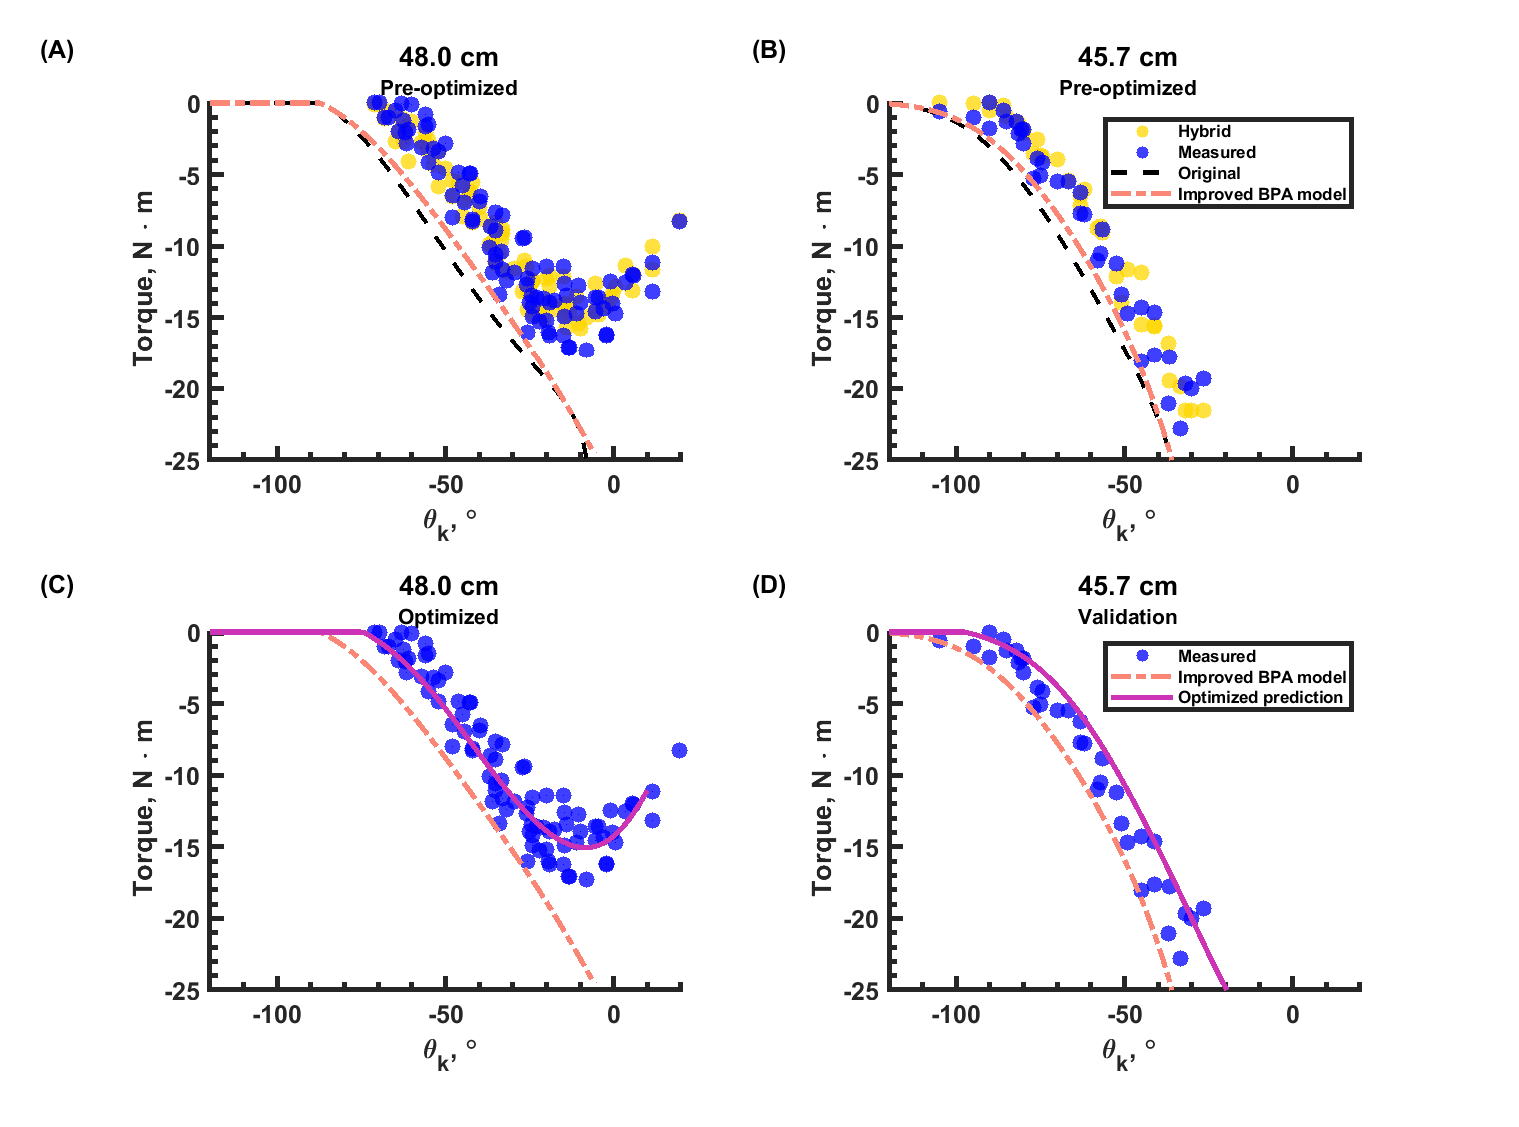
\includegraphics[width=1\textwidth]{FlxPin_group.eps}
\end{center}
\caption{Results for the pinned knee joint using flexor BPAs. Dashed black line shows the torque predicted with our original model. Blue dots are the experimentally measured torque. Yellow dots represent the hybrid method of calculating torque. The magenta line represents the predicted torque.  \textbf{(A)} Measured and pre-optimized torque prediction for the $\qty{48.5}{\cm}$ BPA. \textbf{(B)} Measured and pre-optimized torque prediction for the  $l_{0}=\qty{45.7}{\cm}$ BPA. \textbf{(C)} Theoretical and measured torque for the $l_{0}=\qty{48.5}{\cm}$ BPA using optimization results. \textbf{(D)} Predicted measured torque for the $l_{0}=\qty{45.7}{\cm}$ BPA using the optimization results} \label{fig:FlxPin_group}
\end{figure}
The optimization yielded $\chi_{0} = \qty{11.9}{\mm}$, $\chi_{1} = \qty{102}{\kN\per\m}$, and $\chi_{2} = \qty{10.6}{\kN\per\m}$ (Table~\ref{tab:OptCoeff}). It can be seen that the model with these correction factors greatly improves the ability to predict the joint torque, even capturing the reduction in force at small joint angles that was completely missing from the previous model. The $l_{0}=\qty{45.7}{\cm}$ BPA was used for validation (Fig.~\ref{fig:FlxPin_group}\textbf{D}). It can be seen that the improved model does a good job of predicting the torque with a different muscle length configured to operate over a different joint range of motion. The optimized torque prediction for the $l_{0}=\qty{48.5}{\cm}$ BPA has an $\text{RMSE}=1.616$, $\text{FVU}=0.0958$, and a maximum absolute residual of $3.2527$; validation on the $l_{0}=\qty{45.7}{\cm}$ BPA gives $\text{RMSE}=2.1214$, $\text{FVU}=0.0878$, and a maximum absolute residual of $5.1690$ (Table~\ref{tab:TorqueFit}).

\begin{table}[htbp]
\caption{Optimized coefficient values for flexor and extensor configurations. $\text{X}_0$ is a constant length offset (in meters), $\text{X}_1$ and $\text{X}_2$ are stiffness values (in N/m) in the bracket's X and Y directions, respectively, and $\text{X}_3$ is the unitless wrapping factor.}
\label{tab:OptCoeff}
\fontsize{10pt}{10pt}\selectfont
\begin{tabular}{@{}lrrrr@{}}
\toprule
\textbf{}   &   $\mathbf{X}_0$     &  $\mathbf{X}_1$                   & $\mathbf{X}_2$                   & $\mathbf{X}_3$             \\ \midrule
\multicolumn{1}{l}{\textbf{Flexor}} & \multicolumn{1}{r}{0.0119} & \multicolumn{1}{r}{1.02E+05} & \multicolumn{1}{r}{1.06E+04} & \multicolumn{1}{r}{--} \\ \midrule
\textbf{Extensor}                     & -0.0109                     & 1.02E+05                      & 1.06E+04                      & 0.123                    \\ \bottomrule
\end{tabular}
\end{table}

\subsection{Extensor on Pin Joint}

When the new stiffness and length offet model was used to predict torque for the knee extensor, measured torque was slightly higher than the original model calculates for the \qty{48}{\cm} resting length BPA, while it was slightly lower than expected in the \qty{46}{\cm} BPA, and it was much lower in the \qty{42}{\cm}. Only the $K_{1}$ and $K_{2}$ terms from the previous optimization results were used with the extensor configuration. Firstly, by inspection, the zero point for the measured torque was shifted to the right of the original model, indicating an offset that was at least opposite in sign from the $\chi_{0}$ term in the previous section. Secondly, if we look at the BPA $l_{0}=\qty{46}{\cm}$ as an example, we see good correlation between the hybrid-method calculated torque and the originally predicted torque, but a divergence in the actual measured torque. 

\begin{figure}[htbp]
\begin{center}
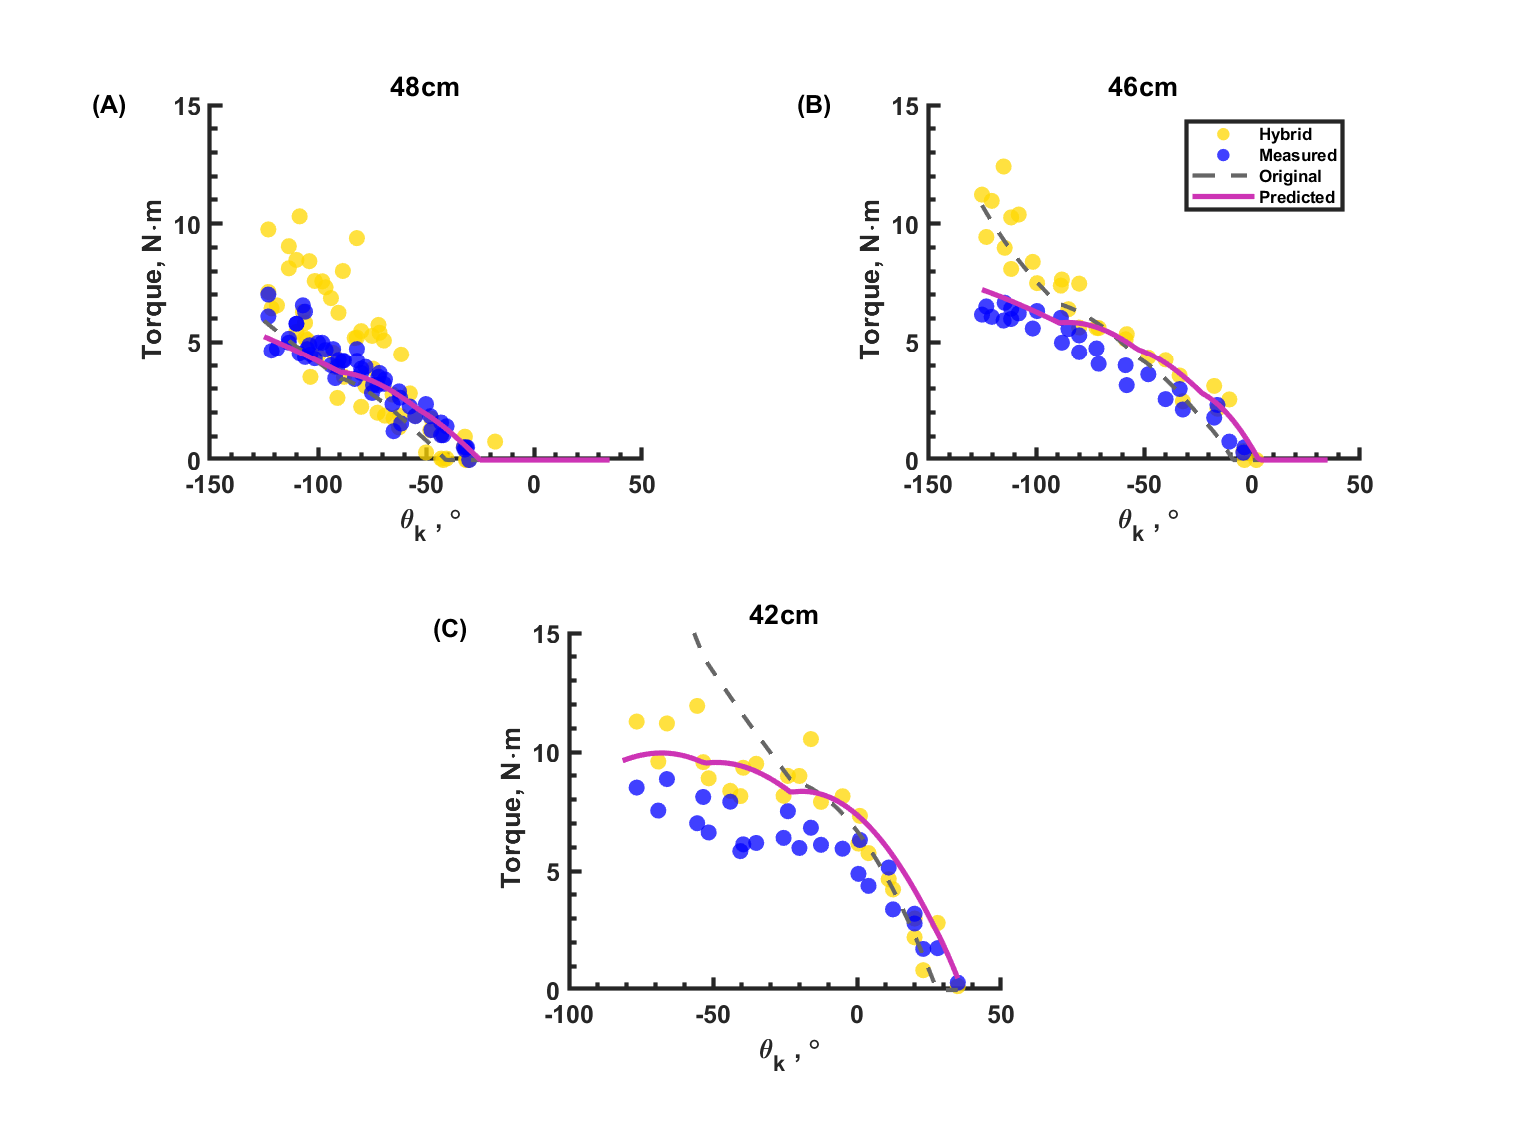
\includegraphics[width=1\textwidth]{ExtPin_group.eps}
\end{center}
\caption{Pinned knee torque versus knee angle with the extensor BPAs. Blue dots are experimentally measured data, yellow dots are hybrid calculated torque, black dashed line is the original predicted values, and magenta line is the optimized predicted torque. For resting lengths, \textbf{(A)} \qty{48.0}{\cm}, \textbf{(B)} \qty{45.7}{\cm}, \textbf{(C)} and \qty{41.5}{\cm}.}\label{fig:ExtPin_group}
\end{figure}

Results are shown in Fig. \ref{fig:ExtPin_group}. The solution was found while holding the $l_{0}=\qty{41.5}{\cm}$ BPA for validation. The optimization resulted in $\chi_{0} = \qty{-10.9}{\mm}$ and $\chi_{3} = 0.123$. It should be noted here that the length offset $\chi_{0}$ is almost equal in magnitude, but opposite sign, as the flexor configuration. The goodness of fit values for the torque prediction is found in table \ref{tab:TorqueFit}. 


\subsection{Extensor on Biomimetic Knee}


We obtained results using the biomimetic knee with a $\phi$\qty{10}{\mm} BPA in the extensor configuration. The bracket frame origin is the centroid of the cantilevered segment that holds the muscle origin bracket to the proximal femur (see Fig. \ref{fig:bktFrame}\textbf{C}, right side). 

%Insert a small paragraph or so on how artificial tendon was used, changing the stiffness equation.

The torque results for a $l_{0}=\qty{52.0}{\cm}$ BPA are shown in Fig. \ref{fig:Ext10mm_52cm}. The torque values measured are significantly smaller than both the original prediction and back-calculated torque using the hybrid method. The results from the previous extensor configuration lead to a better torque prediction. GoF values can be found in table \ref{tab:TorqueFit}. Fig.\ref{fig:Ext_passthru} shows the difficulty of modeling a BPA path that passes through the femoral condyles. Using the optimization results for extensor BPAs on the pinned knee joint, the $l_{0}=\qty{52.0}{\cm}$ BPA has an $\text{RMSE}=0.8920$, $\text{FVU}=0.3396$, and a maximum absolute residual of $1.4188$.

\begin{figure}[htbp]
\begin{center}

\includegraphics[width=1\textwidth]{Ext10mm_52cm.eps}
\end{center}
\caption{Measured versus expected isometric torque results using a $\phi$\qty{10}{mm}, $l_{0}=\qty{51.8}{\cm}$ extensor BPA on the biomimetic knee. Measured results are blue dots. Original prediction is a dashed black line. Optimized prediction is a solid magenta line. Hybrid calculation shown in yellow dots.} \label{fig:Ext10mm_52cm}
\end{figure}

\begin{figure}[htbp]
\begin{center}
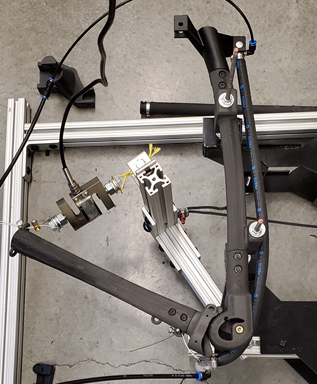
\includegraphics[width=0.65\textwidth]{KneeExt_10mm_passthru.png}
\end{center}
\caption{A configuration that is particularly hard to model. The BPA passes between the femoral condyles close to ICR.}\label{fig:Ext_passthru}
\end{figure}

%Flexor, biomimetic joint, with joint

\subsection{Flexor on Biomimetic Knee}


Fig.~\ref{fig:FlxGrp} shows the isometric torque values of the biomimetic knee from measurements, the Hunt model \citep{hunt_modeling_2017}, and the predictions of the updated model. The values for $\chi_{0}$, $\chi_{1}$, and $\chi_{1}$ derived from the flexors on the pinned knee were used. The bracket frame for the $\phi$\qty{10}{\mm} BPA is shown on the left hand side of Fig. \ref{fig:bktFrame}\textbf{C}, and for the $\phi$\qty{20}{\mm} it is \ref{fig:bktFrame}\textbf{D}. Fig. \ref{fig:FlxGrp}\textbf{A} represents a $\phi$\qty{10}{\mm} $l_{0}=41.5 cm$ BPA with a \qty{21}{\mm} artificial tendon made out of $\phi \qty{1.5}{\mm}$ Shimano bicycle brake cable. The brake cable was wrapped four times. The BPA was pressurized to \qty{604}{\kPa}. The predicted values have an $\text{RMSE}=0.3007$, $\text{FVU} = 0.0102$, and a maximum absolute residual of $0.4647$ $N\cdot m$.  Fig. \ref{fig:FlxGrp}\textbf{B} represents a $\phi$\qty{20}{\mm} $l_{0}=41.5 cm$ BPA with a \qty{15}{\mm} artificial tendon made out of Shimano bicycle brake cable (wrapped six times). Maximum human isometric torque values are shown as the black dotted line. The experiment was performed at \qtylist{620;325}{\kPa}. At \qty{620}{\kPa}, the predicted values have an $\text{RMSE}=1.8024$, $\text{FVU} = 0.0499$, and a maximum absolute residual of $3.5678$ $N\cdot m$. The BPA torque does not exceed the magnitude of the human torque from ca. 60 -- 100 degrees knee flexion. Allowing for a $\pm20\%$ deviation from the human mean, the BPA does not produce human levels of torque from 78 -- 103 degrees knee flexion. 

\begin{figure}[htbp]
\begin{center}
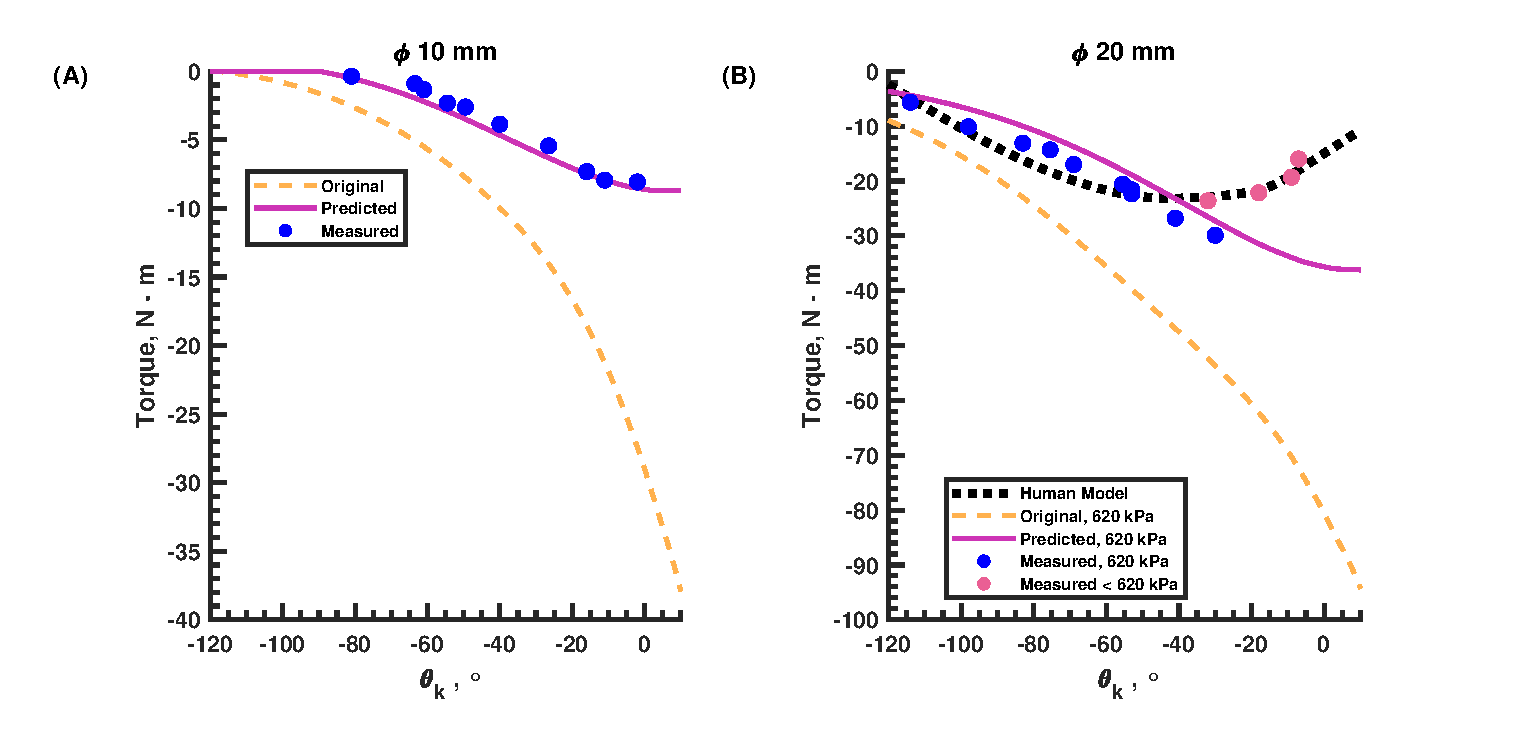
\includegraphics[width=1\textwidth]{FlxGrp.eps}
\end{center}
\caption{Biomimetic knee torque for \textbf{(A)} $\phi$\qty{10}{\mm} $l_{0}=\qty{41.5}{\cm}$ flexor BPA with a \qty{21}{\mm} artificial tendon. Blue dots show the measured torque values. Magenta line is the predicted torque using the improved BPA characterization and optimization from the previous sections. The dashed light orange line shows the torque predicted using only the improved BPA characterization. \textbf{B)} $\phi$\qty{20}{\mm} $l_{0}=\qty{41.5}{\cm}$ flexor BPA with a \qty{15}{\mm} artificial tendon uses the same colors for \qty{620}{\kPa} results. Human values are given as a black dotted line. Due to the BPA exceeding the ultimate strength of the femur, torque measurements were taken at $P<P_{620}$ to show the desired RoM is acheivable. Results for torque measurements at \qtylist{560;421;325;281}{\kPa} (from left to right, respectively), are shown as pink dots.}\label{fig:FlxGrp}
\end{figure}



\begin{table}[htbp]
\caption{Goodness of fit for the improved torque model across test configurations. RMSE and maximum absolute residual are in $\text{N}\cdot\text{m}$.}
\label{tab:TorqueFit}
\begin{tabular}{@{}lccc@{}}
\toprule
\textbf{Configuration} & \textbf{RMSE} & \textbf{FVU} & \textbf{Max.\ residual} \\
\midrule
Flexor, pin joint, $l_{0}=\qty{48.5}{\cm}$ (fit) & 1.616 & 0.0958 & 3.2527 \\
Flexor, pin joint, $l_{0}=\qty{45.7}{\cm}$ (validation) & 2.1214 & 0.0878 & 5.1690 \\
Extensor, biomimetic knee, $l_{0}=\qty{52.0}{\cm}$ & 0.8920 & 0.3396 & 1.4188 \\
Flexor, biomimetic knee, $\phi$\qty{10}{\mm}, $l_{0}=\qty{41.5}{\cm}$ & 0.3007 & 0.0102 & 0.4647 \\
Flexor, biomimetic knee, $\phi$\qty{20}{\mm}, $l_{0}=\qty{41.5}{\cm}$ (\qty{620}{\kPa}) & 1.8024 & 0.0499 & 3.5678 \\
\bottomrule
\end{tabular}
\end{table}

\section{Preliminary Neuromechanical Simulation Recordings}\label{sec:preliminary_sim_results}

The AnimatLab phase-1 run described in Section~\ref{sec:preliminary_sim_methods} produced synchronized joint, neural, contact-sensory, and body-motion recordings over \qty{10}{\second}. Basic checks confirmed finite values and a uniform \qty{0.2}{\milli\second} sampling interval in both exported charts. Each chart contained 50,001 samples from 0 through \qty{10}{\second}; nine trailing zero-filled rows beyond the configured chart end were excluded. Figure~\ref{fig:animatlab_phase1_preliminary} shows bilateral hip, knee, and ankle angles. Neural and contact-sensory recordings remain archived with the run; the contact-sensory channels record membrane voltage rather than contact force. These recordings demonstrate signal acquisition and alternating activity in this run, rather than validated locomotor performance. The model included an externally applied horizontal force during the first second, and neither stable walking nor effective ground-contact gating was established.

\begin{figure}[htbp]
\centering
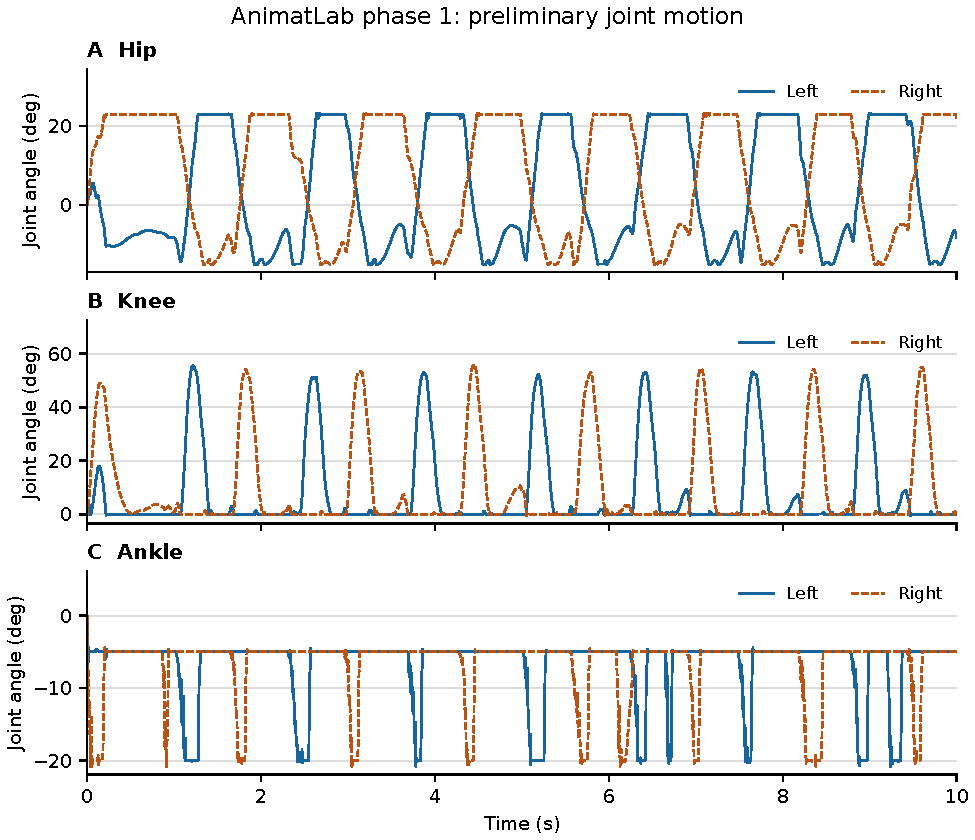
\includegraphics[width=\textwidth,height=0.60\textheight,keepaspectratio]{figs/Preliminary/animatlab_phase1_joint_angles.pdf}
\caption[Preliminary AnimatLab hip, knee, and ankle recordings]{Preliminary AnimatLab phase-1 joint motion: \textbf{(A)} hip, \textbf{(B)} knee, and \textbf{(C)} ankle angles in the model's recorded joint conventions. Blue solid and orange dashed traces denote left and right sides. All 50,001 samples within the configured 0--\qty{10}{\second} chart window are retained without filtering. The model includes an external horizontal force during the first second. These traces document joint motion in an instrumented run; they do not establish stable walking or effective ground-contact gating.}
\label{fig:animatlab_phase1_preliminary}
\end{figure}

\section{Ongoing Experiments}\label{sec:ongoing}

At the time of this writing, two additional sets of isometric knee torque experiments are in progress, and space is reserved here for their results.

First, the flexor configuration of the pinned knee joint is being extended from a single BPA to two parallel BPAs. Parallel flexor grouping mimics the coordinated action of biological knee flexors and is expected to increase available flexor torque at high flexion angles, where the single-muscle configuration fell short of human isometric torque values (Section~\ref{sec:results_torque}). The improved torque model of Section~\ref{sec:improved_model} will be refit with the two-muscle arrangement, and the resulting torque predictions will be validated against measured data.

Second, the model optimization is being revisited using a surrogate optimization approach in place of the multiobjective genetic algorithm, which is expected to reduce the computation time required to fit the compliance and wrapping terms and to improve the conditioning of the parameter estimates.

% TODO: Insert results for the two-BPA flexor configuration and the surrogate
% optimization run here once the test series is complete.


\chapter{Discussion}\label{ch:discussion}

{\doublespacing\normalsize\upshape
\noindent Publication note: Sections~\ref{sec:disc_effects}--\ref{sec:disc_bio} and the associated figures and tables appeared in \citet{bolen_2026} (Bolen, Elzein, Pang, and Hunt, \emph{Actuators}, 2026). Section~\ref{sec:disc_error} is also the subject of an unpublished manuscript in preparation by Bolen, Burgess, Morrow, Elzein, Pang, Scharzenberger, and Hunt \citep{bolen_isometric_2025}. This manuscript has not been submitted for publication. Author contributions for both works are stated in Chapter~\ref{ch:methods}.\par}


\section{Effects of Resting Length}\label{sec:disc_effects}
We have developed new $F_{620}$ equations for \qtylist{10;20}{\mm} diameter Festo BPAs that capture the change in maximum force produced by the actuators at  \qty{620}{\kPa} as a function of their resting length. When examining Equation~(\ref{eq:Fmax10}) and measured data in Figure~\ref{fig:Fmax_fit}b, it can be seen that as $l_0$ goes to infinity, $F_{620_{10}}$ goes to \qty{470}{\N}. When the Festo tool \citep{lang_robert_musclesim_2005} was queried at $l_0=\qty{1}{m}$ as an approximation of infinity, it predicts the $\phi$\qty{10}{\mm} BPA can produce $F=\qty{490}{\N}$ at $P_{620}$. This is within the 10\% variability that Festo states may occur in manufacturing tolerances. Similarly, the Festo data predict a $\phi$\qty{20}{\mm} BPA will produce $F=\qty{1570}{\N}$. Our results for Equation~(\ref{eq:Fmax20}) show that  $F_{620_{20}}$ goes to \qty{1460}{\N} as $l_0$ approaches infinity. Although the difference is much larger, it is also with the \mbox{10\% manufacturing tolerance. }

Where our measured data differs significantly from the Festo model, is that as $l_0$ goes to zero. For the measured data, as the length gets smaller, the force does as well, whereas the Festo tool predicts exponential force increase (see Figure~\ref{fig:Fmax_fit}). As a specific example, when specifying $l_0=\qty{112}{\mm}$ for the \qtylist{10}{\mm} diameter BPAs, the Festo predicted $F_{620}$ is \qtylist{498.6}{\N}. However, using Equation~(\ref{eq:Fmax10}), $F_{620}$ is calculated to be \qtylist{335.3}{\N}. Actual force in the $l_0=\qty{112}{\mm}$ was measured at \qtylist{350.9}{\N} Therefore, the error in predicted $F_{620}$ for the $\phi$\qty{10}{\mm} BPA is $4.5\%$ for our model and $42.1\%$ using the Festo tool. Researchers using BPA resting lengths under \qty{300}{\mm} should take note of these results.

\citet{festo_2026} (p.~12) states that force will be reduced by approximately 10\% for a minimum nominal length. In \citet{festo_2018} (p.~14) they say the force can deviate by 10\% based on factors such as: production variation, material variation, and deviation from nominal length ($l_0$). \citet{festo_2013} (p.~13) notes that testing was done with BPAs that are ten times the uninflated diameter, and that theoretical force can increase by up to 10\%. In each datasheet, the characteristic curves appear to be the same. As demonstrated above, the \qty{100}{\mm} $\phi$\qty{10}{\mm} BPA should have much less force than what is shown in the curve. This is our experience and the reason for the testing. It is unclear why the MuscleSIM tool \citep{lang_robert_musclesim_2005} then predicts higher force as resting length decreases. It could be a reversed sign coefficient in their internal curve-fit model. We have shown here that as the nominal length goes to zero, so does force. 

The reason for BPA models predicting higher force than what is measured experimentally is a recurrent theme across many models: they do not account for the end effects of the pressure vessel where end effects dominate.	Nominally, the clamped ends fix the inner and outer diameter while allowing axial and radial displacement. In the isometric case, there is only radial displacement. The boundary conditions force steep gradients in stress and strain near the ends. Near the boundary conditions are where axial, radial, and circumferential strains deviate from analytic solutions to a cylindrical model. For a constant pressure, the end effect region appears to have the same length. Therefore, in shorter BPAs, the end effects dominate. The axial length scale of the boundary section is comparable to $l_0$,  and the active force differs substantially from that of an assumed perfect cylinder.

Manufacturing variations seem to play an important factor in the behavior of these actuators. It remains to be seen how $\epsilon_{620}$ can be known a priori. We still suspect that it is a function of $l_0$, but it might also be a function of other factors such as product batch number or UV light exposure \citep{festo_2026} (p.~15); \citep{festo_2018} (p.~6); \citep{festo_2013} (p.~13). We found there to be larger variations in the \qtylist{10}{\mm} BPAs than in the \qtylist{20}{\mm} BPAs. Modeling work of ideal McKibben actuators describe how the relationship between contraction and initial length is a function of the total number of twists and the angle of twist in the usable muscle area \citep{chou_measurement_1996}. It is unclear if there are variations in the angle and number of twists in the Festo BPAs due to manufacturing. Uncovering the relationship between $\epsilon_{620}$ and $l_0$ for the Festo DMSP artificial muscles, if it exists in a meaningful way, will require additional controlled tests. 

Similarly, it is not clear how the maximum force might change with manufacturing variations. This was reasonably corrected for by normalizing the equations to each individual's maximum contraction, but more nuanced details might emerge with more data collection. Not knowing these relationships a priori means there is still a need for robots and other systems to go through an iterative design stage if it is discovered that the system does not produce the torque or have the RoM that the design team expects. However, the data and models provided here should enable for faster redesigns with fewer \mbox{additional measurements.}


\section{Nondimensionalized Force Prediction}

We have also introduced the concept of nondimensionalized isometric force that is a function of relative strain and relative pressure (Equation~(\ref{eq:Fstar})). This elegant equation has only three coefficients with low error (see Table~\ref{tab:Fstar}). In the work presented here, we introduce the relative pressure term, $P^*=P/P_{620}$. Our data show that by normalizing force, contraction, and pressure, we are able to create a simplified force equation as a function of contraction and pressure that scales well with initial actuator length, as expressed by Equation~(\ref{eq:force}) in Section~\ref{sec:force_model}.

For example, given $l_0=\qty{54}{\mm}$ and $P=\qty{300}{\kPa}$, the measured force was \mbox{$F_{actual} = \qty{103}{\N}$.} Force prediction using only the Festo tool predicts the force to be \mbox{$F_{predict} = \qty{270}{\N}$.} This is $161\%$ greater than the measured force. Using Equations~(\ref{eq:Fmax10}) and~(\ref{eq:Fstar}) with Equation~(\ref{eq:force}) gives $F_{predict} = F^*(0, 0.48) \cdot F_{620}(0.054) = 0.49 \cdot \qty{230}{\N} = \qty{112}{\N}$. This is an error of $8\%$, which is much more accurate than using the Festo tool only.

The presented work is capable of predicting force output for 10 mm and 20 mm muscles with different initial muscle lengths, internal pressure, and contraction amount with minimal initial data collection. However, it remains to be seen if these relationships are maintained over the full lifecycle of the muscles. There are not yet any peer reviewed studies investigating the long-term behavior of these artificial muscles, though the Festo datasheet provides some indication of what can be expected \citep{festo_2026} (p.19). They report that the 40 mm BPA can complete 1 million cycles at \qty{6000}{\N} (maximum rated load), or 10 million cycles at \qty{4000}{\N}. The service life of the other size BPAs is not reported; however, it is mentioned that thermal stressing may reduce the lifespan and they should be inspected every 500,000 cycles for signs of aging \citep{festo_2018} (pp.~10--11). Future research should look at the behavior of these muscles over time.

In our work, $P_{620}=\qty{620}{\kPa}$ is the maximum supply pressure for our system, and other users of this actuator may use a different supply pressure. However, this supply pressure is not required, and normalizing by this value was chosen as a method for improving the optimization techniques by reducing the sensitivity of the term associated with pressure. This equation will work for any pressure supplies below \qty{620}{\kPa}. We also anticipate the equation will also work for pressures up to \qty{800}{\kPa} (the maximum rated pressure for Festo $\phi$\qty{10}{\mm} BPAs); however, we do not have the data to confirm this.

\section{Comparison with Other Published BPA Models}

The proposed model was compared with the formulations by \citet{sarosi_new_2012}, \citet{sarosi_10mm}, and \citet{martens_modeling_2017}, to evaluate their predictive performance across actuator sizes and operating conditions (see Table~\ref{tab:model_compare} and Figure~\ref{fig:ModelCompare}).
For the $\phi$\qty{20}{\mm} BPA, parameters from \cite{sarosi_new_2012} were used, corresponding to actuators with resting lengths of \qty{200}{\mm} and \qty{400}{\mm}. These were compared against the experimental data at $l_0=\qty{300}{\mm}$ and $l_0=\qty{450}{\mm}$, respectively. For the $\phi$\qty{10}{\mm} BPA with resting lengths of \qty{257}{\mm} and \qty{233}{\mm}, parameters from \cite{sarosi_10mm} were applied. In each case, the maximum contraction parameter ($k_{max}$) was determined numerically by solving $F(\qty{6.2}{\bar}, k_{max}) = 0$, ensuring consistency with the experimental maximum pressure condition.




\begin{table}[H]
\caption{Goodness-of-fit comparison for the Bolen, Sárosi, and Martens and Boblan models at different resting lengths (in mm) for \qty{10}{\mm} and \qty{20}{\mm} BPAs. RMSE and maximum error are reported in newtons, and FVU denotes the fraction of variance unexplained.}
\label{tab:model_compare}
\tiny
\begin{adjustwidth}{-2cm}{0cm}
%\centering %% If there is a figure in wide page, please release command \centering
\begin{tabularx}{\textwidth}{@{}lllllllllll@{}}
\toprule
\textbf{Diameter} &
  \textbf{Length} &
  \textbf{} &
  \textbf{Bolen} &
  \textbf{} &
  \textbf{} &
  \textbf{Sarosi} &
  \textbf{} &
  \textbf{} &
  \multicolumn{2}{l}{\textbf{Martens and Boblan}} \\ 
\textbf{} &
  \textbf{} &
  \textbf{RMSE} &
  \textbf{FVU} &
  \textbf{Max. Error} &
  \textbf{RMSE} &
  \textbf{FVU} &
  \textbf{Max Error} &
  \textbf{RMSE} &
  \textbf{FVU} &
  \textbf{Max. Error} \\ \midrule
\textbf{10 mm} & 257 & 22.9 & 0.0353 & 46.0  & 143.8 & 1.3903 & 235.8 & 73.8  & 0.3668 & 122.9  \\
\textbf{}      & 233 & 16.8 & 0.0187 & 30.3  & 132.7 & 1.1655 & 222.6 & 62.6  & 0.2590 & 101.2  \\ \midrule
\textbf{20 mm} & 300 & 35.6 & 0.0144 & 114.0 & 132.1 & 0.1992 & 313.4 & 72.8  & 0.0605 & 137.8  \\
\textbf{}      & 450 & 67.6 & 0.0258 & 166.6 & 177.7 & 0.1785 & 294.8 & 862.1 & 4.2022 & 1321.1 \\ \bottomrule
\end{tabularx}
\end{adjustwidth}
\end{table}

While the \citet{sarosi_new_2012} and \citet{sarosi_10mm} models capture general trends in force–contraction behavior, discrepancies were observed when applying parameters derived from different actuator lengths. In particular, the model tends to over-predict force at higher pressures and low amounts of contraction, suggesting sensitivity to geometric scaling effects not explicitly accounted for in the formulation.

The \citet{martens_modeling_2017} model  is derived from a geometric and material-based framework and provides a more physically grounded representation of actuator behavior. However, its accuracy depends strongly on precise geometric parameters, including braid angle, wall thickness, and fiber length. Small deviations in these parameters can lead to significant differences in predicted force, particularly at higher pressures.

\begin{figure}[H]%[tbp]
%\begin{adjustwidth}{-\extralength}{0cm}
%\centering
%\begin{center}
    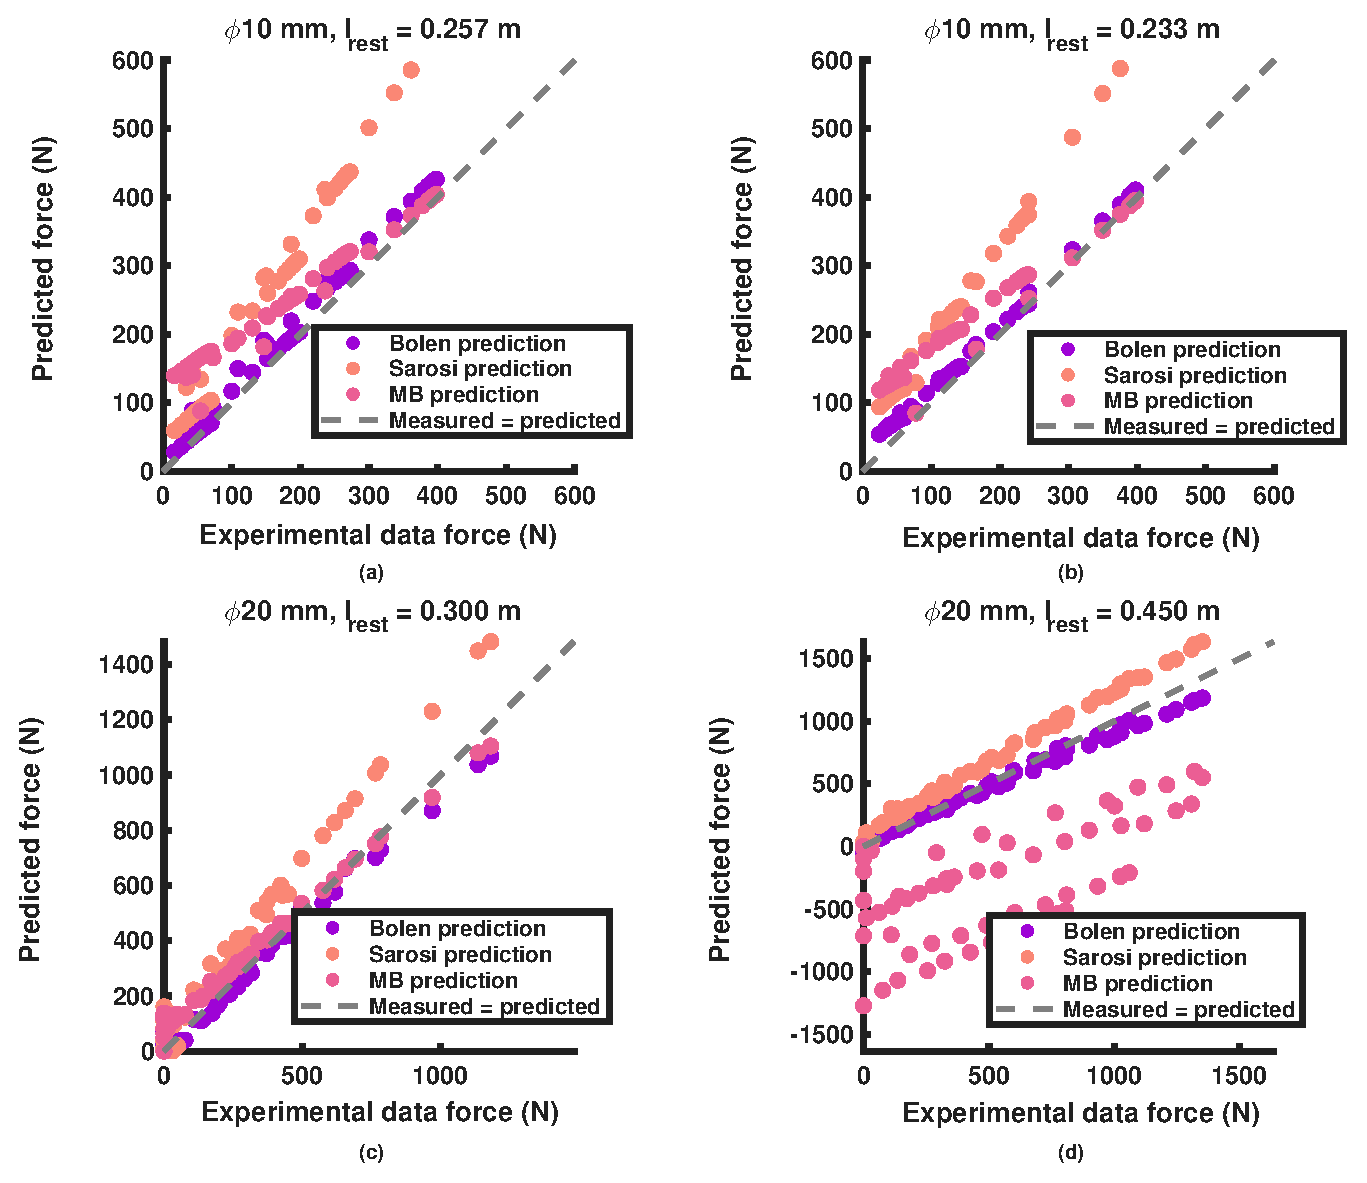
\includegraphics[width=.99\textwidth]{05_Comparison.eps}
%\end{center}
%\end{adjustwidth}
\caption{Comparison between measured and predicted BPA force at varying amounts of contraction and pressure. A $y=x$ perfect fit line is added for reference. The BPAs compared are: (\textbf{a}) $\phi$\qty{10}{\mm}, $l_0=\qty{0.257}{\mm}$, (\textbf{b}) $\phi$\qty{10}{\mm}, $l_0=\qty{0.233}{\mm}$, (\textbf{c}) $\phi$\qty{20}{\mm}, $l_0=\qty{0.300}{\mm}$, and (\textbf{d}) $\phi$\qty{20}{\mm}, $l_0=\qty{0.450}{\mm}$.}\label{fig:ModelCompare}
\end{figure}

The Martens and Boblan model was first evaluated at the same pressure–contraction points as in their experimental data \citep{martens_modeling_2017} (Tables A1 and  A2), indicating that it reproduces the general published force map shape but is sensitive to the assumed initial geometry. Examining their $\phi$\qty{20}{\mm} BPA, for example, using the explicitly stated $l_0=\qty{300}{\mm}$ and initial diameter $D_{0}=\qty{20}{\mm}$ significantly under-predicted the results compared to using the implied $l_0=\qty{296}{\mm}$ (\citep{martens_modeling_2017} (Table A1)) and $D_{0}+H_{0}=\qty{21.8}{\mm}$, where $H_{0}=\qty{1.8}{\mm}$ is the material thickness. The diameter adjustment can be implied \mbox{from \citep{chou_measurement_1996}.} This adjusted diameter was also included for the $\phi$\qty{10}{\mm} BPA to give a better fit. As can be seen in Figure~\ref{fig:ModelCompare} and Table~\ref{tab:model_compare}, the highest accuracy is observed when $\phi$\qty{20}{\mm} and $l_0=\qty{300}{\mm}$, which is at or very near their experimental measurements. For the $\phi$\qty{10}{\mm} BPAs the accuracy decreases even though their experimentally measured $l_0=\qty{250}{\mm}$ is close to our $l_0=\qty{257}{\mm}$ and $l_0=\qty{233}{\mm}$. The largest error occurs at $\phi$\qty{20}{\mm} and $l_0=\qty{450}{\mm}$ and the model starts to predict negative force. We have calculated that the $F_{PE}\cdot\frac{dD}{DL}$ term becomes very large compared to the others \citep{martens_modeling_2017} (p.~5). This suggests that the model is sensitive to geometric parameter selection and interpretation, particularly with respect to initial length and diameter definitions.

In comparison, the present normalized model demonstrates improved consistency across actuator lengths by incorporating experimentally derived scaling through $F_{620}$ and $\epsilon_{620}$. This normalization reduces sensitivity to geometric variation and enables a unified representation of actuator behavior, while maintaining predictive accuracy over the tested range of pressures and contractions.


\section{Implications for Real-Time Control and Simulation}

Although pneumatic muscle actuators exhibit hysteresis, thermodynamic effects, and other dynamic behavior, accurate and high-performance controller designs can still be achieved using a static force map approach when the underlying static force model is accurate. Martens and Boblan explicitly note that BPA dynamics are often dominated by the air dynamics inside the actuator and the mass flow behavior of the valve, such that precise modeling of the static force characteristic remains crucial for torque control \mbox{accuracy \citep{martens_modeling_2017}.} This view is consistent with more recent BPA control work, including a sensor-less torque control interface for BPA-driven joints \citep{martens_framework_2018}, stable force/position/stiffness control of antagonistic pneumatic-muscle joints \citep{ugurlu2019stable, hunt_development_2017}, and sensor-less angle stiffness control of antagonistic BPA systems \citep{shinSensorlessAngleStiffness2022}. 

In this context, the present model is well suited for real-time use because it reduces the static isometric force prediction to a low-order normalized surface, $F^*(\epsilon^*,P^*)$, scaled by the resting-length-dependent term $F_{620}(l_0)$. This structure is computationally inexpensive to evaluate online and is also suitable for lookup-table implementation. While the present work does not model the full actuator--valve dynamics, it provides the static force relationship needed as a feedforward or inner-model component in real-time torque control, simulation, and preliminary design workflows. It is anticipated that improved real-time control for high-speed and high-precision systems will benefit more from improved modeling of airflow dynamics than dynamics involving actuator hysteresis, damping, and other dynamic behavior. Characterizing the actuators under dynamic operating conditions --- isokinetic (constant-velocity), isobaric, and isotonic (constant-load) contractions --- is a natural next step beyond the isometric characterization reported here, for which the pressure--force dynamics model of \citet{elzein_pressure_2025} provides the modeling foundation.



\section{Biomimetic Artificial Muscle Analogy}\label{sec:disc_bio}

BPA artificial muscles are often said to be analogous to biological muscles because they have force--length curves and can produce force only in tension. This analogy is worth closer inspection. For example, the describes the passive force–length curve has been described as an exponential function arising from connective tissue elements, while the active force–length relationship is typically modeled as a bell-shaped curve reflecting actin–myosin overlap \citep{winters1990}. These formulations emphasize that muscle force generation is governed by nonlinear geometric and material interactions rather than simple linear elasticity.
McKibben-type pneumatic artificial muscles (of which Festo is an example) exhibit analogous nonlinear behavior, though arising from fundamentally different physical mechanisms. As shown by Chou and Hannaford, the force–length relationship of McKibben actuators is derived from geometric constraints imposed by the braided shell, leading to a nonlinear dependence of force on actuator length through the braid angle \cite{chou_measurement_1996}. In their formulation, actuator force is proportional to pressure and a nonlinear geometric term $(3\cos^2\theta - 1)$, which governs both the maximum contraction limit and the curvature of the force–length relationship. The work presented here demonstrates that this nonlinear curve can be well approximated by an exponential as well.

However, there are some distinct differences between how these artificial muscles behave when compared to biological muscles.
For example, the biological muscle optimum fiber length $l_{OFL}$ is not equivalent to $l_0$ in the muscles. The maximum active force that the artificial muscles can produce is at the resting length, also the maximum length, of the artificial muscles. In contrast, the maximum active force a biological muscle length can produce is somewhere in the middle of the total contractile length of the muscle. 

Furthermore, biological muscles can adapt the optimal operating length through structural remodeling (e.g., sarcomere addition or tendon compliance) while BPAs have a fixed geometric configuration. This allows biological systems to self-optimize for the particular tasks the animal is subjected to. In order to re-optimize a robot for new tasks, new actuators would have to be swapped into the system. This distinction highlights a key limitation of BPAs in biomimetic applications, while also reinforcing the importance of accurate nonlinear modeling for control and design.




\section{Sources of Error in Isometric Torque Generation}\label{sec:disc_error}

Our improved BPA characterization predicts torque more accurately than the original BPA model (see Fig.~\ref{fig:FlxPin_group}\textbf{A} and \ref{fig:FlxPin_group}\textbf{B}). This only accounts for part of the error. There are certainly many factors that affect the torque results. Compliance in the testing system, position location tolerance, flexibility of brackets, imperfect path modeling, and variation in individual BPAs are other factors.

Simplifying the model and testing it allowed us to see how we were deficient in our previous analysis. The isometric system is not rigid. There is compliance in the winch cable, artificial tendons, and brackets that bend and stretch. We introduced a constant length offset term $\chi_{0}$, axial stiffness $\chi_{1}$, and bending stiffness $\chi_{2}$. The bracket frame of reference was placed where it starts to cantilever and is rotated about $Z$.  Optimization found results for a $\phi$\qty{10}{\mm} BPA with $l_{0}=\qty{48}{\cm}$ in the simple pinned knee configuration. These results were validated with second $\phi$\qty{10}{\mm} BPA with $l_{0}=\qty{45.7}{\cm}$.

The modeling of extensor BPA paths that wrap around the knee joint is an approximation with inherent error (Fig. \ref{fig:Ext_passthru}). When the moment arm is short, small changes to it can have a large effect on the resultant torque \citep{young_analyzing_2019}. It was assumed that wrapping the BPA around the joint would be easier to account for than adding a patella, deterministically designing its location as a function of knee angle, and accounting for friction. During greater magnitude knee flexion angles, shorter $l_{0}$ BPAs were noted as being stretched and compressed (see Fig.~\ref{fig:testJigs}\textbf{C}). The same force that caused the stretch and compression would also sometimes cause the BPA to slip off of the anterior bolt head of the bolt that holds the femur to the knee. This would result in a $\pm \; 20\,\text{mm}$ displacement in the $Z$ direction, which means a change the force vector and a change in torque. The system designer, too, must be mindful. Fig. \ref{fig:ExtPin_group} shows a deviation between measured and originally predicted results that widens as expected torque increases. This indicates system compliance. However, the  hybrid calculated torque matching or exceeding predicted torque, except for higher degrees of flexion in the $l_{0}=\qty{42}{\mm}$, indicates a loss of functional $l_m$. BPA This is why the $\chi_{3}$ term was created in \eqref{eq:deltaL}. Fig. \ref{fig:ExtPin_group} shows the improved fit from running the optimization that includes this term.

The biomimetic knee joint with an extensor BPA was used to validate the extensor optimization results. The predicted line more closely matches the torque values. However, the predicted torque is still higher than experimentally measured torque.


In the presented nonlinear biomimetic robotic system, rigid body mechanics simplifications, often encountered in other robotic and biomechanical systems, are removed. Instead, working from the simple to the complex elucidated mechanisms of system compliance that will lead to much more accurate first iteration designs. Technologies have been developed to predict system bending and axial compliance, a constant length offset, and a loss of usable length that occurs as artificial muscle bends around a joint. 

In equation $m\ddot \varepsilon^* + c (\dot \varepsilon^* ) \dot \varepsilon^* + k ( \varepsilon^* ) \varepsilon^* = F$ given $k(\varepsilon^{*}, P^{*})
= \left.\frac{\partial F}{\partial \varepsilon^{*}}\right|_{P^{*}}
= -c_{0}c_{1}e^{-c_{1}\varepsilon^{*}}
  - 2c_{2}\varepsilon^{*}P^{*}e^{-c_{2}(\varepsilon^{*})^{2}}$
then if we set mass m and external force F to zero we get
$c (\dot \varepsilon^* ) = (k ( \varepsilon^* ) \varepsilon^*)/\dot \varepsilon^*$


\section{Synthesis: From Actuator Characterization to Neuromechanical Control}\label{sec:synthesis}

Taken together, the actuator and joint level results of this dissertation form a coherent design chain for biomimetic legged robots. At the actuator level, the maximum isometric force of Festo BPAs was shown to depend strongly on resting length, correcting a systematic over-prediction by the manufacturer's tool at short resting lengths, and a nondimensional force surface was derived that predicts isometric force from relative strain and relative pressure with only three diameter-dependent coefficients. At the joint level, the improved actuator model was combined with a compliance-corrected musculotendon kinematics model to predict isometric knee torque across the full range of motion for pinned and biomimetic knee joints, and the biomimetic knee driven by optimized BPAs was shown to meet or exceed human isometric torque over most of the range of motion.

This chain was developed deliberately so that each stage can feed the next. The force model supplies the actuator terms for the torque model; the torque model supplies the plant model for designing joint controllers; and the validated biomimetic knee demonstrates that the actuator architecture can reproduce human joint-level force capabilities, which is a prerequisite for the neuromechanical control studies planned in Chapter~\ref{ch:futurework}. What remains missing is the neural layer itself: a controller that schedules the measured muscle forces the way the nervous system schedules motor unit activity. The AARL's prior AnimatLab walker (Section~\ref{sec:prior_walker}) offers an early demonstration of both halves of that challenge: acting as a feedforward controller, its two-layer CPG drove gait-like stepping of a suspended biomechanical model --- confirming that rhythm generation does not require sensory feedback --- but untuned afferent feedback could not support those patterns against the ground, which is why feedback tuning is the critical path from feedforward stepping to weight-bearing walking. Closing that loop in simulation, and finally on hardware, is the subject of the next chapter.

\chapter{Future Work}\label{ch:futurework}

The experimental work of Chapters~\ref{ch:methods}--\ref{ch:results} characterizes the plant: the actuators and the joints they drive. The remaining task of the dissertation project is the controller --- a synthetic nervous system that schedules those actuators the way the nervous system schedules muscles --- and eventually the physical robot that the controller runs on. This chapter lays out the planned work in four stages: a neuromechanical simulation pipeline (Section~\ref{sec:fw_pipeline}), a two-layer CPG with full proprioceptive and contact feedback (Section~\ref{sec:fw_cpg}), extension of the sensorium with vestibular, ocular, and cerebellar contributions (Section~\ref{sec:fw_senses}), and physical realization on a treadmill robot with real-time neural control (Section~\ref{sec:fw_hardware}). Some of the work described here is planned for the remainder of the dissertation; the later stages extend naturally into postdoctoral research.

\section{A Neuromechanical Simulation Pipeline}\label{sec:fw_pipeline}

The first stage converts the validated biomechanical design into a physics simulation that a neural controller can drive. The pipeline has three parts.

\subsection{From OpenSim to MuJoCo}

The starting point is the author's modified OpenSim model: the Gait2392-derived robot variant in which the actuator set has been reduced and adapted to the BPA hardware and the muscle origin, insertion, and wrapping points have been updated to the optimized robot routing \citep{bolen_determination_2019, morrow_optimization_2020}. The model will be kept in OpenSim 4.x format and converted to MuJoCo \citep{todorov_mujoco_2012} using MyoConverter \citep{caggiano_myosuite_2022, wang_myosim_2022}, which converts OpenSim musculoskeletal models to MuJoCo models with optimized muscle kinematics and kinetics. The conversion will be sanity-checked by inspecting the generated model, verifying joint naming and ordering for later sensor and actuator mapping, confirming that the expected number of muscle-tendon actuators exists with plausible attachment geometry, and fixing any conversion gaps by revising the OpenSim model or accepting manual edits in the MuJoCo model.

The MuJoCo model will represent actuation with muscle-like actuators that carry an internal activation state, so that SNS outputs can drive them through activation dynamics. Each timestep, MuJoCo updates the kinematics and the muscle variables (e.g., muscle-tendon lengths and velocities) needed to compute proprioceptive signals.

\subsection{Coupling the Synthetic Nervous System}

The neural controller will be implemented with SNS-Toolbox \citep{nourse_sns_2023}, which supports large networks of spiking and non-spiking neurons and couples directly to MuJoCo. At each timestep, SNS receives Ia, Ib, and II proprioceptive channels plus binary heel and toe contact signals from the MuJoCo model, processes them through the neural core described below, and returns per-muscle activation commands that are fed into the MuJoCo muscle activation states.

The coupling will be brought up incrementally. Before any gains are tuned against human gait, the mechanics-only loop will be verified with open-loop activation patterns, confirming the sign and magnitude behavior of torques and forces. The SNS will then be added with a minimal sensor set --- contact signals plus a single proprioceptive channel --- and only later expanded to the full Ia/Ib/II set. Once stable, the activation strengths and neuron-to-muscle mapping parameters will be tuned across a few walking speeds. A Simscape-based mechanical plant could substitute for MuJoCo for validation of specific mechanical subsystems, but Simscape does not natively host the spiking and non-spiking neuron models of an SNS, so MuJoCo remains the primary platform.

\section{A Two-Layer CPG with Sensory Feedback}\label{sec:fw_cpg}

\subsection{Architecture}

The neural core follows the two-level organization of the mammalian locomotor CPG established by the Rybak group \citep{rybak_modelling_2006, mccrea_organization_2008, rybak_organization_2015}: each leg has a rhythm generator (RG) circuit, which produces the basic locomotor rhythm and controls its period, and a pattern formation (PF) circuit, which shapes the rhythm into phase-appropriate activation of the flexor and extensor motoneuron populations. A left--right rhythm generator circuit coordinates the two legs through commissural inhibition and excitation, following the models of left--right coordination \citep{molkov_mechanisms_2015, danner_central_2016}. The per-leg PF output drives the motoneuron pools --- here, the BPA activation commands for the hip, knee, and ankle muscle groups of each leg.

\subsection{Sensory Feedback Channels}

Three classes of proprioceptive feedback will close the loop between the MuJoCo plant and the CPG, mirroring the biological afferents organized in the Sensory Afferent Database \citep{bolen_sensory_2023}:

\begin{itemize}
    \item \textbf{Ia afferents} (muscle spindle primary endings) signal muscle length and velocity, providing stretch reflex pathways and phase-dependent modulation of the PF network.
    \item \textbf{Ib afferents} (Golgi tendon organs) signal muscle force, providing load-dependent regulation of stance-phase extensor activity.
    \item \textbf{II afferents} (muscle spindle secondary endings) signal length, contributing to position sensing and interjoint coordination.
    \item \textbf{Contact receptors} on the heel and toe provide discrete stance and swing boundary signals, driving phase transitions and weight-support switching.
\end{itemize}

\subsection{Verification Tests}

Before attempting locomotion, the network will be verified with simple simulation tests in which tonic stimulus is applied to the muscle motoneurons, to the pattern-formation layer, and to the rhythm-generator layer, and the resulting outputs are compared with the corresponding experimental literature. The closest biological analogue is the tonic-stimulation air-stepping protocol of Selionov et al. \citep{selionov_tonic_2009}, in which tonic central and sensory stimuli facilitate involuntary stepping in humans; analogous deletion and stimulation phenomena are reproduced by the two-level CPG model itself \citep{rybak_modelling_2006} and by neuromechanical implementations \citep{markin_afferent_2010, shevtsova_modeling_2016}. Comparing the simulated tonic-stimulation responses with these studies will validate the sign, gain, and phase structure of the implemented circuits before any walking-speed tuning is attempted.

\section{Extending the Sensorium: Vestibular, Ocular, and Cerebellar Contributions}\label{sec:fw_senses}

Once stepping is stable, three supraspinal contributions will be added. First, vestibular feedback will be simulated with IMU-like sensing of body orientation and angular velocity, extending the lab's balance-platform work, in which an inverted pendulum with pseudo-vestibular IMU feedback maintained balance on an oscillating platform \citep{bolen_balance_2024, bolen_selfbalancing_2024} and analytic neural networks reproduced human balance dynamics \citep{hilts_dynamic_2019}. Second, ocular feedback will be modeled to investigate how visual stabilization cues can help reset IMU drift --- a well-known practical problem for inertial sensing on robots --- by treating visual measurements of the horizon and surrounding as a low-frequency correction to the vestibular estimate. Third, a cerebellar layer will be explored as an adaptive gateway between higher-level locomotion commands and the CPG: a structure that can gate between different gaits or movement patterns (e.g., walking, running, turning) and tune the phase relationships among them, in line with the cerebellum's established role in adaptation and coordination. The proprioceptive--vestibular interaction literature \citep{akay_relative_2021} will guide how these signals are weighted.

\section{Physical Realization: A Treadmill Robot with Real-Time Neural Control}\label{sec:fw_hardware}

The final stage returns to hardware. The robot will walk on a treadmill with real-time feedback and control implemented on a embedded computing stack: Teensy microcontrollers for the low-latency per-joint loops (valve control, pressure sensing, contact sensing), and an Nvidia Jetson-class companion computer for the SNS network evaluation and activation computation. A serial connection to a host computer will be used only for data logging and high-level commands (e.g., run, walk, stimulate a named neural pathway), keeping the control loop fully embedded. This division of labor mirrors the SNS-Toolbox backend philosophy, which targets embedded computing platforms for real-time neural simulation \citep{nourse_sns_2023}.

Because the static force and torque models of Chapters~\ref{ch:methods}--\ref{ch:results} are computationally inexpensive lookup-table candidates, they will serve as the feedforward plant model inside the real-time controller, while the dynamic pressure--force behavior under pulse-modulated control will draw on the state-space model of \citet{elzein_pressure_2025}. Embedded execution of the complete CPG-plus-reflex network on this stack is the intended demonstration of the dissertation project: a robot that walks with human-like biomechanics under a biologically grounded neural controller, and whose nervous system --- unlike a living animal's --- can be instrumented, stimulated, and lesioned at will.

\section{Toward Dynamic Whole-Body Maneuvers}\label{sec:fw_kickflip}

Beyond steady walking, the long-term goal of this line of research is dynamic, whole-body maneuvering: transitions between gaits, reactive balancing, and ultimately ballistic maneuvers that require coordinating the full actuator set through brief, precisely timed activation bursts. The author's aspiration for this program is a robot that can perform a kickflip --- a maneuver that, like its skateboard namesake, demands explosive coordinated extension, precise timing, aerial body orientation, and controlled landing. It is exactly the kind of behavior that exercises every layer of the proposed architecture, from contact receptors and spinal pattern generation to vestibular orientation sensing and cerebellar coordination, and it would demonstrate that biomimetic actuation and neuromechanical control scale from steady locomotion to dynamic whole-body movement.

\chapter{Conclusion}\label{ch:conclusion}

This dissertation moved the biomimetic humanoid robot project from an unvalidated design concept to a quantitatively characterized actuator set and a validated knee-level biomechanical design, and it defined the path from those experimental foundations to neuromechanical control.

At the actuator level, the analysis in Chapters~\ref{ch:methods} and~\ref{ch:results} produced novel equations for calculating isometric force in Festo \qtylist{10;20}{\mm} diameter BPAs. The work elucidated the relationship between maximum BPA force at \qty{620}{\kPa} and resting length, $F_{620}(l_0)$, a previously unreported characteristic of these actuators that the manufacturer's tool predicts with the wrong trend, and it produced a nondimensional force surface, $F^*(\epsilon^*,P^*)$, with only three diameter-dependent coefficients. Taken together, these fits predict isometric BPA force across resting lengths from a small number of measurements, correct the large over-predictions of the manufacturer's tool at short resting lengths, and outperform published single-length models. In a design workflow, these equations make it possible to select actuator diameter and resting length, and to evaluate whether a proposed muscle routing can meet force and range-of-motion requirements, before committing to a prototype.

At the joint level, the improved actuator model was combined with a compliance- and wrapping-corrected musculotendon kinematics model and validated on two knee designs. The hybrid torque calculation method isolated the sources of error between prediction and measurement, and the resulting correction terms --- a constant length offset, series compliance represented by an equivalent stiffness, and a wrapping loss term --- substantially improved torque prediction on the pinned knee and transferred to the biomimetic four-bar knee. The biomimetic knee driven by optimized BPAs was shown to meet or exceed human isometric knee torque over most of the range of motion, confirming that the optimized muscle routing of the author's earlier work is realizable in hardware, and identifying the high-flexion regime where additional flexor capacity is needed.

Beyond the specific models, the dissertation's methodological contribution is the actuator-to-joint design chain itself: characterize the actuator, correct for the compliance and geometry of the transmission, validate against human biomechanics, and only then close the loop with a controller. The remaining gap --- the neural layer --- is scoped in Chapter~\ref{ch:futurework}: a MuJoCo plant converted from the lab's OpenSim models via MyoConverter, wrapped in an SNS-Toolbox synthetic nervous system implementing a two-layer CPG with per-leg rhythm generation and pattern formation, left--right coordination, and Ia, Ib, II, and contact feedback, verified first by tonic-stimulation tests against the literature, then extended with vestibular, ocular, and cerebellar layers, and finally deployed on embedded hardware controlling a treadmill-walking robot. The biomimetic platform that results will permit neuromechanical experiments --- neural lesions, sensory deletions, pathway stimulation --- that are impossible in living animals, closing the cycle between better robots and better biological understanding, and opening the way toward dynamic whole-body maneuvers.

% Terminal bibliography for the monograph-style dissertation.
% All citations resolve against thesis.bib; the bibliography is
% single-spaced per the psutex class redefinition.

\bibliographystyle{plainnat}
\bibliography{thesis}


%-------------------------Appendices-----------------------------
% NOTE: \backmatter removed 2026-09-08 --- it suppressed the appendix chapter
% counter, so sections/tables/equations numbered ".1" and "(1)" instead of
% "A.1"/"(A1)" (PSU ETD appendix lettering). The heading-number guard in
% psutex.cls prevents a duplicated "A" before the "Appendix A:" titles.
\appendix
% Appendix-scoped numbering: A.1 sections, (A1) equations, Table A1/B1 style
\renewcommand{\theequation}{\thechapter\arabic{equation}}
\renewcommand{\thetable}{\thechapter\arabic{table}}
\renewcommand{\thefigure}{\thechapter\arabic{figure}}
\chapter{Appendix A: Muscle Force and Joint Torque Calculations}\label{app:muscle_calcs}

% TODO: This appendix will contain the supplementary derivations for the
% muscle force and joint torque calculations used in Chapters 3-5, including
% the moment-arm projection method and the vector geometry of the muscle paths.

[To be completed.]

\chapter{Appendix B: Neuron Model Equations}\label{app:neuron_equations}

This appendix documents the neuron and synapse models used by the synthetic nervous systems in this project, both in the AnimatLab walker model and in the SNS-Toolbox implementation of the MuJoCo pipeline (Chapter~\ref{ch:futurework}). The authoritative model state is the working AnimatLab project file (\texttt{Biped\_2xCPG\_wSubs/Biped\_2xCPG\_wSubs.aproj}); after the network reorganization described in Section~\ref{sec:preliminary_sim_methods}, a fresh standalone export (\texttt{Biped\_2xCPG\_wSubs\_Standalone.asim}) runs headless and carries the rhythm-generator charts, and the earlier phase-1 instrumented export (\texttt{walk new new tester added 2 axis\_phase1.asim}) records the run reported in Section~\ref{sec:preliminary_sim_results}.

\section{Spiking Neuron Model}

Each spiking neuron is a conductance-based leaky integrator with threshold and adaptation,
\begin{equation}
    C_{m}\,\dot{V} \;=\; -\,g_{\text{leak}}\left(V - E_{\text{rest}}\right)
                      \;+\; I_{\text{syn}} \;+\; I_{\text{app}},
    \label{eq:app_membrane}
\end{equation}
where $V$ is the membrane potential, $C_{m}$ the membrane capacitance ($g_{\text{leak}} = C_{m}/\tau_{m}$ with membrane time constant $\tau_{m}$), $E_{\text{rest}}$ the resting potential, $I_{\text{syn}}$ the summed synaptic current, and $I_{\text{app}}$ any applied (tonic stimulation) current. A spike is emitted when $V$ exceeds the firing threshold, after which $V$ resets and an after-hyperpolarization (AHP) of amplitude $A_{\text{AHP}}$ with time constant $\tau_{\text{AHP}}$ is applied; the threshold itself accommodates with the firing history (relative accommodation $r_{\text{acc}}$, time constant $\tau_{\text{acc}}$). Optional calcium channels are defined but disabled in the current model ($G_{\text{max,Ca}} = 0$).

The parameter values shared by the neurons in the walker model are given in Table~\ref{tab:app_neuron}.

\begin{table}[htbp]
\caption{Spiking neuron parameters in the AnimatLab bipedal walker model
(\texttt{Biped\_2xCPG\_wSubs}). All neurons share these values except the motor
neuron threshold noted below.}
\label{tab:app_neuron}
\begin{tabular}{@{}lll@{}}
\toprule
\textbf{Parameter} & \textbf{Symbol} & \textbf{Value} \\
\midrule
Resting potential        & $E_{\text{rest}}$   & \qty{-60}{\mV} \\
Membrane time constant   & $\tau_{m}$          & \qty{5}{\ms}   \\
Initial firing threshold & $V_{\text{th}}$     & \qty{-55}{\mV} (motor neurons: \qty{-59}{\mV}) \\
Relative accommodation   & $r_{\text{acc}}$    & 0.3            \\
Accommodation time const & $\tau_{\text{acc}}$ & \qty{10}{\ms}  \\
AHP amplitude            & $A_{\text{AHP}}$    & \qty{1}{\mV}   \\
AHP time constant        & $\tau_{\text{AHP}}$ & \qty{3}{\ms}   \\
\bottomrule
\end{tabular}
\end{table}

\section{Non-Spiking (Graded) Chemical Synapses}

Pattern-formation and motoneuron-drive connections in the walker use graded chemical synapses, whose conductance is a clipped linear ramp of the presynaptic potential,
\begin{equation}
    g_{\text{syn}}(V_{\text{pre}})
    \;=\; g_{\text{max}}\;
    \operatorname{clamp}\!\left(
        \frac{V_{\text{pre}} - V_{\text{th}}}{V_{\text{sat}} - V_{\text{th}}},
        \,0,\,1\right),
    \qquad
    I_{\text{syn}} = g_{\text{syn}}\left(V_{\text{post}} - E_{\text{syn}}\right),
    \label{eq:app_nonsyn}
\end{equation}
where $V_{\text{th}}$ and $V_{\text{sat}}$ are the synaptic threshold and saturation potentials and $E_{\text{syn}}$ the reversal potential. The walker model instantiates three non-spiking synapse types:

\begin{itemize}
    \item \textbf{Nicotinic ACh (excitatory drive):}
          $E_{\text{syn}} = \qty{-10}{\mV}$,
          $g_{\text{max}} = \qty{0.5}{\micro\siemens}$,
          $V_{\text{th}} \to V_{\text{sat}} = \qty{-65}{\mV} \to \qty{-20}{\mV}$.
    \item \textbf{Hyperpolarizing IPSP (inhibition):}
          $E_{\text{syn}} = \qty{-70}{\mV}$,
          $V_{\text{th}} \to V_{\text{sat}} = \qty{-55}{\mV} \to \qty{-40}{\mV}$.
    \item \textbf{Depolarizing IPSP:}
          $E_{\text{syn}} = \qty{-55}{\mV}$,
          $V_{\text{th}} \to V_{\text{sat}} = \qty{-60}{\mV} \to \qty{-40}{\mV}$.
\end{itemize}

Spiking chemical synapses and electrical synapses (rectifying coupling weight 0.1, non-rectifying 0.2) are also defined in the model and are available for the sensory afferent pathways of the MuJoCo/SNS implementation.

\section{Relation to the SNS-Toolbox Implementation}

These are the standard AnimatLab firing-rate/conductance models. SNS-Toolbox \citep{nourse_sns_2023} implements corresponding classes of non-spiking and spiking neurons with conductance-based synapses, and the AnimatLab parameters above served as the physically motivated initialization for the first SNS-Toolbox instantiation of the spinal network: a 406-neuron network with per-leg rhythm-generator half-centers, phase-shifted pattern-formation groups, motoneuron pools for all 92 muscle-tendon actuators of the converted model, and Ia, Ib, and II afferent populations. In that implementation the non-spiking membrane and graded-synapse equations take the same forms as Equations~(\ref{eq:app_membrane}) and~(\ref{eq:app_nonsyn}) with the spiking threshold and accommodation terms removed, and the afferent resting-tone offsets are zeroed so that Ia and Ib signals are pure activity measures; the rhythm-generator layer has been verified to oscillate at a human-like period with the two legs in antiphase under tonic drive (Section~\ref{sec:fw_cpg}). An explicit parameter-mapping and validation campaign between the two implementations remains future work; the tonic stimulation tests of Section~\ref{sec:fw_cpg} correspond to constant $I_{\text{app}}$ injections into Equation~(\ref{eq:app_membrane}) at the motoneuron, pattern-formation, and rhythm-generator layers respectively.


\chapter{Appendix C: Model Geometry, Bracket Frames, and Compliance Parameters}\label{app:model_geometry}

This appendix documents the numeric geometry and compliance parameters behind the torque models of Chapters~\ref{ch:methods}--\ref{ch:results} as they exist in the project's MATLAB code, with file names given so that any value can be traced to the code that produced it. Route and bracket coordinates are coded in meters and reported here in millimeters; stiffnesses are coded and reported in newtons per meter. The bracket reference points are interpretation choices for the 3D-printed (Onyx FDM) attachment hardware, set from CAD by the author; moving a reference point changes the identified stiffness values, so the points are recorded here alongside the values they produced.

\section{Static BPA Pathway Data}

The static BPA model routes each actuator as a straight-segment polyline through via points stored in a per-test \texttt{Location} array of dimensions $M\times3\times N$, where $N$ is the number of joint frames in the motion sweep and $M$ the number of via points; the first row in the distal link frame is marked by a cross-point index. There are no binormal or surface-frame quantities: at each frame the force direction is the normalized vector from the cross-point row to the previous row transformed into the crossing frame, $\hat{\mathbf{u}} \propto \mathbf{R}^{-1}\,\mathbf{p}_{C-1} - \mathbf{p}_{C}$ [Provenance: \texttt{Testing\_Data/2022\_02\_Festo/minimizeFlxPin2brk.m} lines 429--440; \texttt{minimizeFlxPin.m} lines 381--394; \texttt{minimizeExtX3.m} lines 676--687; BPA struct fields, \texttt{minimizeFlxPin.m} lines 28--35]. The pinned-knee test routes are archived as \texttt{FlxPinBPASet.mat} (5 flexor tests, $M=2$, knee angle $-120^{\circ}$ to $+10^{\circ}$) and \texttt{ExtPinBPASet.mat} (9 extensor tests, $M=7$, knee angle $-125^{\circ}$ to $+35^{\circ}$).

Table~\ref{tab:app_flxpin_tests} lists the five pinned-knee flexor tests; their routes are two points, femur-frame origin $\mathbf{p}_{1} = [-75.0,\,100.0,\,32.8]$~mm and tibia-frame insertion $\mathbf{p}_{2} = [-50.1,\,-45.0,\,32.3]$~mm (test 1; \texttt{FlxPinBPASet.mat}, kf(1), frame 1). Table~\ref{tab:app_extpin_route} lists the extensor pinned-knee route of test 1 at $\theta_{k}=-125^{\circ}$; rows 1--6 are femur-frame and row 7 is tibia-frame, and as the knee extends, rows 2--6 release onto $\mathbf{p}_{1}$ (wrap released at $+35^{\circ}$). Table~\ref{tab:app_extpin_tests} lists the per-test constants of the nine extensor tests; the validation pool used for the correction terms of Section~\ref{sec:improved_model} is tests \{1, 2, 5, 6, 7, 8\} [Provenance: \texttt{crossPredictFlx.m} line 46].

\begin{sidewaystable}
\caption{Pinned-knee flexor test BPA constants (\texttt{FlxPinBPASet.mat}; test labels from \texttt{minimizeFlxPin10mm\_2brk.m} line 42). All tests use $\phi$\qty{10}{\mm} BPAs; \texttt{fitn} is the end-cap fitting length.}
\label{tab:app_flxpin_tests}
\begin{tabular}{@{}llllll@{}}
\toprule
\textbf{Test} & $\boldsymbol{l_{0}}$ (m) & Tendon (m) & $P$ (kPa) & $F_{m}$ (N) & \textbf{Notes} \\
\midrule
48\,cm        & 0.485 & 0     & 605.7 & 443.4 & \\
46\,cm        & 0.457 & 0     & 614.2 &       & \\
47\,cm        & 0.479 & 0     & 623.2 &       & \\
40\,cm-tendon & 0.406 & 0.035 & 623.4 &       & \\
41\,cm        & 0.410 & 0     & 615.4 &       & \\
\bottomrule
\end{tabular}
\end{sidewaystable}

\begin{sidewaystable}
\caption{Biomimetic knee, extensor 20\,mm BPA route seed (femur frame: p1--p5; tibia frame: p6--p9; \texttt{buildKneeExtContext20mm.m} lines 349--384, Ben-set SolidWorks points). Release schedule of the verified elimination: p5 at $-91.1^{\circ}$, p4 at $-50.4^{\circ}$, p6 at $-47.8^{\circ}$, p7 at $-20.2^{\circ}$, p3 at $+6.1^{\circ}$.}
\label{tab:app_ext_seed}
\begin{tabular}{@{}lrrrll@{}}
\toprule
\textbf{Point} & $x$ (mm) & $y$ (mm) & $z$ (mm) & \textbf{Frame} & \textbf{Role} \\
\midrule
p1 & 40.00 & 35.00  & 0 & femur & BPA origin (attachment) \\
p2 & 83.90 & $-274.76$ & 0 & femur & BPA contacts mounting base \\
p3 & 66.34 & $-427.24$ & 0 & femur & femoral contact \\
p4 & 51.52 & $-446.74$ & 0 & femur & femoral condyle contact \\
p5 & 38.26 & $-453.01$ & 0 & femur & femoral condyle contact \\
p6 & 69.85 & 34.33  & 0 & tibia & tibial contact (upper) \\
p7 & 73.50 & 19.13  & 0 & tibia & tibial contact (mid) \\
p8 & 71.98 & $-12.23$ & 0 & tibia & tibial contact (lower) \\
p9 & 34.06 & $-66.87$ & 0 & tibia & patellar ligament ring (distal, pEnd) \\
\bottomrule
\end{tabular}
\end{sidewaystable}

\begin{table}[htbp]
\caption{Pinned-knee extensor BPA route of test 1 at $\theta_{k}=-125^{\circ}$ (\texttt{ExtPinBPASet.mat}, ke(1), frame 1; mm).}
\label{tab:app_extpin_route}
\begin{tabular}{@{}lrrr@{}}
\toprule
\textbf{Point} & $x$ (mm) & $y$ (mm) & $z$ (mm) \\
\midrule
p1 & 30.00  & $-50.00$ & 0 \\
p2 & 65.00  & $-350.00$ & 0 \\
p3 & 42.40  & $-408.50$ & 0 \\
p4 & 28.20  & $-421.60$ & 0 \\
p5 & 10.50  & $-425.20$ & 0 \\
p6 & $-8.60$ & $-422.80$ & 0 \\
p7 & 42.50  & $-75.90$ & 0 \\
\bottomrule
\end{tabular}
\end{table}

\begin{table}[htbp]
\caption{Pinned-knee extensor test BPA constants (\texttt{ExtPinBPASet.mat}, ke(2)--ke(9); test 1: $l_0 = 0.400$~m, tendon 0, $P = 624.9$~kPa, $F_m = 436.3$~N). All tests use $\phi$\qty{10}{\mm} BPAs.}
\label{tab:app_extpin_tests}
\begin{tabular}{@{}llll@{}}
\toprule
\textbf{Test} & $\boldsymbol{l_{0}}$ (m) & Tendon (m) & $P$ (kPa) \\
\midrule
40\,cm-tendon & 0.400 & 0.040 & 605.2 \\
42\,cm        & 0.420 & 0     & $\sim$620 \\
42\,cm-tendon & 0.420 & —     & $\sim$620 \\
43\,cm        & 0.430 & 0     & $\sim$620 \\
43\,cm-tendon & 0.430 & —     & $\sim$620 \\
46\,cm        & 0.460 & 0     & $\sim$620 \\
47\,cm        & 0.470 & 0     & $\sim$620 \\
48\,cm        & 0.480 & 0     & $\sim$620 \\
\bottomrule
\end{tabular}
\end{table}

The biomimetic flexor route (\texttt{buildKneeFlexorContext20mm.m}) is a three-point path --- femur-frame origin $\mathbf{p}_{1}$, a moving wrap point $\mathbf{p}_{\text{wrap}}$ on the tibia, and tibia-frame insertion $\mathbf{p}_{\text{end}}$ --- with the wrap point held on a standoff surface of radius \texttt{bpaRb} about the joint and its $z$ placed on the projected $\mathbf{p}_{1}$--$\mathbf{p}_{\text{end}}$ line; the optimizer seed is $\mathbf{p}_{1,0} = [-50.0,\,35.0,\,50.0]$~mm and $\mathbf{p}_{2,0} = [-12.24,\,-8.87,\,27.87]$~mm with $l_{0} = 415$~mm and 25~mm tendon [Provenance: \texttt{buildKneeFlexorContext20mm.m} lines 96--119, 179--188; \texttt{buildKneeFlexorRoute20mm.m} lines 99--186]. The biomimetic extensor seed route is given in Table~\ref{tab:app_ext_seed}, including the release schedule of the route-elimination rule.

\section{Joint Transformation Matrices}

The knee transform is planar: every joint frame is a rotation about $z$ by the knee angle $\varphi$ composed with a translation fitted to robot CAD tables of the migrating instantaneous center of rotation. With $\mathbf{R} = \mathbf{R}_{z}(\varphi)$, the robot (femur$\to$ICR) transform is $\mathbf{T}_{\text{Pam}} = [\mathbf{R},\; [f_{3}(\varphi),\,f_{4}(\varphi),\,0]^{\top};\; \mathbf{0}^{\top}\;1]$ with $f_{3}, f_{4}$ cubic-spline fits (ICR $x$: 23.30 to 10.47~mm; $y$: $-416.65$ to $-395.66$~mm over $\varphi = 0.17$ to $-2.62$~rad), and the ICR$\to$tibia transform is the pure translation $[f_{13}(\varphi),\,f_{14}(\varphi),\,0]^{\top}$ ($x$: 29.66 to $-7.58$~mm; $y$: 25.97 to 22.33~mm), composed as $\mathbf{T}_{t1\!\to\!f} = \mathbf{T}_{t1\!\to\!\text{ICR}}\;\mathbf{T}_{\text{Pam}}^{-1}$ over 100 frames spanning $\varphi \in [-120^{\circ}, +10^{\circ}]$ [Provenance: \texttt{buildKneeFlexorContext20mm.m} lines 34--80; \texttt{buildKneeExtContext20mm.m} lines 30--78; \texttt{Functions/ModernRobotics/RpToTrans.m}]. In the archived test sets the per-frame transform maps tibia to femur/ICR; at $\theta_{k}=-120^{\circ}$ (test kf1),
\begin{equation}
    \mathbf{T}_{k} \;=\;
    \begin{bmatrix}
    -0.5000 & 0.8660 & 0 & 0.0045\\
    -0.8660 & -0.5000 & 0 & -0.3958\\
    0 & 0 & 1 & 0\\
    0 & 0 & 0 & 1
    \end{bmatrix},
    \label{eq:app_Tk}
\end{equation}
i.e., $\mathbf{R}_{z}(-120^{\circ})$ with constant translation $[4.5,\,-395.8,\,0]$~mm, rotating to $\mathbf{R}_{z}(+10^{\circ})$ at full extension (\texttt{FlxPinBPASet.mat}, kf(1)).

\section{Bracket Reference Points and Frames}

Table~\ref{tab:app_bracket_points} lists the bracket reference points. Each compliant bracket carries an instantaneous body-fixed frame anchored at its reference point, constructed by two rotations (yaw about $z$, then pitch about the yawed $y$): with $\mathbf{p}_{b}$ the vector from the reference point to the bracket-to-BPA attachment target, $\theta_{br} = \operatorname{atan2}(p_{by}, p_{bx})$, $\mathbf{R}_{kbr} = \mathbf{R}_{z}(\theta_{br})\,\mathbf{R}_{y}(\phi_{br})^{\top}$ with $\phi_{br} = \operatorname{atan2}(p'_{bz}, p'_{bx})$ measured on the yawed vector $\mathbf{p}'_{b} = \mathbf{R}_{z}^{\top}\mathbf{p}_{b}$, and $\mathbf{T}_{kbr} = [\mathbf{R}_{kbr},\, \mathbf{p}_{br};\, \mathbf{0}\;1]$; the frame's $x$ axis therefore aims along the nominal load path. The angles are computed per configuration from the bracket geometry, not fixed [Provenance: \texttt{minimizeFlxPin2brk.m} lines 175--203; \texttt{minimizeExtX3.m} lines 463--474]. Force is transformed into the bracket frame by $\mathbf{RowVecTrans}(\mathbf{T}_{kbr}^{-1}, \mathbf{F}_{k})$ and deformed points are mapped back by $\mathbf{RowVecTrans}(\mathbf{T}_{kbr}, \cdot)$. The single-rotation (yaw-only) variant used in the earlier one-transform fit survives in \texttt{minimizeFlxPinX3.m} line 205.

\begin{table}[htbp]
\caption{Bracket reference points (mm, as coded; divided by 1000 in code). All are Ben-set CAD interpretation points; frame denotes the frame the vector is expressed in.}
\label{tab:app_bracket_points}
\begin{tabular}{@{}lrrll@{}}
\toprule
\textbf{Point} & $x$ & $y$ & $z$ & \textbf{Configuration / meaning} \\
\midrule
Pbri & $-27.50$ & $-107.81$ & $-0.54$ & pinned-knee flexor, insertion bracket (knee-ICR frame) \\
Pbr2 & $-52.61$ & 0 & 75.06 & pinned-knee flexor, origin-side 2nd bracket (hip frame) \\
Pbr  & $-3.84$  & $-46.44$ & 62.50 & pinned-knee extensor, rib midpoint, medial side (hip frame) \\
Pbr  & 8.38 & 20.75 & 25.10 & biomimetic extensor 10\,mm, cantilever centroid \\
Pbr  & 9.48 & $-33.38$ & 33.90 & biomimetic flexor 20\,mm, bolt-pattern centroid \\
Pbr  & $-19.00$ & 22.00 & 27.60 & biomimetic flexor 10\,mm, cantilever centroid \\
\bottomrule
\end{tabular}
\end{table}

\section{Stiffness Arrays and Compliance}

Every configuration models bracket compliance as a diagonal Hooke-law spring in the bracket frame, $\mathbf{K}_{br} = \operatorname{diag}(k_{1}, k_{2}, k_{3})$ newtons per meter, with the scalar compliance projected onto the force-path unit vector, $c_{b} = \hat{\mathbf{u}}\,\mathbf{K}_{br}^{-1}\hat{\mathbf{u}}^{\top}$, exactly as in Equations~(\ref{eq:bktstiffness})--(\ref{eq:keff}). The per-configuration stiffness arrays and their series combinations are given in Table~\ref{tab:app_stiffness_arrays}; when an artificial tendon is present its axial spring ($\times2$ cables, effective steel area $1.51\times10^{-6}$~m$^{2}$, $E = 193$~GPa) adds in series, $c_{\text{eff}} = c_{b} + c_{\text{ten}}$ ($+\,c_{b2}$ for the second bracket), and the force balance $F_{\max}F^{*}(\varepsilon^{*}(\delta), P^{*}) = k_{\text{eff}}\,\delta$ is solved per frame by \texttt{fzero} on the contraction interval [Provenance: \texttt{minimizeFlxPin2brk.m} lines 284--339, 489--499; \texttt{minimizeFlxPin.m} lines 266--275; \texttt{minimizeExtX3.m} lines 562--570; \texttt{minimizeExt.m} line 352; \texttt{minimizeFlx.m} line 314].

\begin{table}[htbp]
\caption{Bracket stiffness arrays by configuration ($K = [k_{1}, k_{2}, k_{3}]$ in bracket-frame axes, N/m; optimizer solves $X_{1}, X_{2}$ assigned as shown).}
\label{tab:app_stiffness_arrays}
\begin{tabular}{@{}lll@{}}
\toprule
\textbf{Configuration} & $\boldsymbol{K}$ array & \textbf{Source} \\
\midrule
Pinned flexor, single bracket       & $[X_{1},\,X_{2},\,X_{2}]$ & \texttt{minimizeFlxPin.m} line 266 \\
Pinned flexor, insertion bracket    & $[X_{1},\,X_{2},\,X_{1}]$ & \texttt{minimizeFlxPin2brk.m} line 284 \\
Pinned flexor, origin bracket       & $[X_{2},\,X_{1},\,X_{2}]$ & \texttt{minimizeFlxPin2brk.m} line 298 \\
Pinned extensor (with $X_{3}$)      & $[X_{2},\,X_{1},\,X_{2}]$ & \texttt{minimizeExtX3.m} line 562 \\
Biomimetic extensor                 & $[X_{1},\,X_{2},\,X_{2}]$ & \texttt{minimizeExt.m} line 352 \\
Biomimetic flexor                   & $[X_{1},\,X_{2},\,X_{2}]$ & \texttt{minimizeFlx.m} line 314 \\
\bottomrule
\end{tabular}
\end{table}

The wrapping-loss term $X_{3}$ (Equations~\ref{eq:deltaL}--\ref{eq:x3}) is evaluated as $X_{3}\,R\,\lvert\Delta\theta\rvert\,\zeta^{2}$ per contact arc. On the pinned extensor the two physical contact arcs use $R_{1} = 12$~mm ($27^{\circ}$ to $-23^{\circ}$) and $R_{2} = 40$~mm, with arc-length normalizers $27.75/(ang_{1} - ang_{2})$ and $92.46/(ang_{2}+120^{\circ})$; on the biomimetic configurations the bend measure is $w_{\text{rap}}\lvert\theta_{\text{turn}}\rvert$ with $w_{\text{rap}} = 25$~mm [Provenance: \texttt{minimizeExtX3.m} lines 333--359; \texttt{buildKneeFlexorRoute20mm.m} line 268; \texttt{MonoPamDataExplicit\_balanceX3.m} lines 489--494]. The optimizer parameterization is $[100\,X_{0}\ (\text{cm}),\ \log_{10}X_{1},\ \log_{10}X_{2},\ \ldots]$ with bounds $X_{0}\in[0, 20]$~mm and $X_{1}, X_{2}\in[5\times10^{3}, 5\times10^{7}]$~N/m for the flexor; the extensor refit locks $(X_{1}, X_{2})$ to the flexor values and solves $X_{0}\in[-20, 0]$~mm and $X_{3}\in[0, 1]$, enforcing a single stiffness pair across configurations [Provenance: \texttt{minimizeFlxPin10mm\_2brk.m} lines 62--63, 402--404; \texttt{minimizeExt10mmX3.m} lines 46--47; \texttt{sweepExtX3.m} lines 59--60].

\section{Adopted Correction-Term Values}

Table~\ref{tab:app_xi_values} records the correction-term values adopted by the archived code at the time of writing. The pinned-knee fits of record for the published comparison are those of \texttt{minimizeExtPin10\_results\_20260819\_2transforms\_Z2.mat}; the current redesign operating point (context builders \texttt{buildKneeFlexorContext20mm.m} lines 150--165 and \texttt{buildKneeExtContext20mm.m} lines 150--160) pairs the two-bracket flexor fit with an extensor refit in which $(X_{1}, X_{2})$ are locked to the flexor values. Regenerating the results files updates this table.

\begin{table}[htbp]
\caption{Correction-term values of record and current operating point. $(X_{1}, X_{2})$ are shared across flexor and extensor in the current operating point.}
\label{tab:app_xi_values}
\begin{tabular}{@{}llll@{}}
\toprule
\textbf{Term} & \textbf{Pinned fit of record} & \textbf{Current operating point} & \textbf{Source (.mat)} \\
\midrule
Flexor $X_{0}$ (m)   & ---                & $1.647\times10^{-6}$ & crossPredict\_20260907 \\
Flexor $X_{1}$ (N/m) & ---                & $2.107\times10^{6}$  & crossPredict\_20260907 \\
Flexor $X_{2}$ (N/m) & ---                & $1.065\times10^{4}$  & crossPredict\_20260907 \\
Extensor $X_{0}$ (m) & $-1.220\times10^{-2}$ & $-2.364\times10^{-3}$ & both \\
Extensor $X_{1}$ (N/m) & $1.508\times10^{4}$ & $= $ flexor        & both \\
Extensor $X_{2}$ (N/m) & $1.218\times10^{4}$ & $= $ flexor        & both \\
$X_{3}$ (--)         & 0.2937             & 0.4637 (refit)       & both \\
\bottomrule
\end{tabular}
\end{table}



\end{document}
